%%%%%%%%%%%%%%%%%%%%%%%%%%%%%%%%%%%%%%%%%%%%%%%%%%%%%%%%%%%%%%%%%%%%%%%%%%%%%%%
%%%%%%% ColdADC Testing Results
%%%%%%%%%%%%%%%%%%%%%%%%%%%%%%%%%%%%%%%%%%%%%%%%%%%%%%%%%%%%%%%%%%%%%%%%%%%%%%%

\documentclass[10pt]{article}

\topmargin=-0.5in
\oddsidemargin=0in
\evensidemargin=0in
\textwidth=6.2in
\textheight=9.25in

\usepackage[dvips]{graphics}
\usepackage{rotating}
\usepackage{amssymb,amsmath}
\usepackage{graphicx}
\usepackage{cite}
\usepackage{color}
\usepackage[table]{xcolor}
\usepackage{colortbl}
\usepackage{enumerate}

%% draftwatermark causes infinite loop on SL6's ancient TeXLive
%\usepackage[firstpage]{draftwatermark}
\usepackage{lipsum}
\usepackage{tikz}

\usepackage[T1]{fontenc}
\usepackage[utf8]{inputenc}
\usepackage[blocks,affil-it]{authblk}

\RequirePackage{lineno}

\bibliographystyle{plain}
\bibliographystyle{unsrt}

\usepackage{graphicx, subfigure}
\usepackage[colorlinks=true,urlcolor=black,linkcolor=black,citecolor=black,bookmarks=true]{hyperref}

\setcounter{tocdepth}{3}

%% Added by M. Dabrowski
\usepackage{caption}
%\usepackage{subcaption}

\begin{document}
%\linenumbers

\title{DUNE ColdADC ASIC Preliminary Testing Results}

\date{\today}
%\date{January 10, 2020}
\author{}
% The author list in authblk format

\author[3]{D.~Braga}
\author[1]{H.~Chen}
\author[3]{D.~Christian}
\author[1]{M.~Dabrowski}
\author[1,3]{G.~Deptuch}
\author[5]{D.~Dwyer}
\author[1]{J.~Fried}
\author[4]{I.~Furic}
\author[1]{S.~Gao}
\author[5]{C.~Grace}
\author[3]{J.~Hoff}
\author[3]{S.~Holm}
\author[5]{C.~Lin}
\author[2]{Y.~Lu}
\author[2,5]{K.~Luk}
\author[1]{E.~Lopriore}
\author[1,3]{S.~Miryala}
\author[5]{T.~Prakash}
\author[3]{A.~Shenai}
\author[1]{E.~Vernon}
\author[1]{J.~Zhang}

\affil[1]{Brookhaven National Lab., Upton, NY 11973-5000, USA}

\affil[2]{University of California (Berkeley), Berkeley, CA 94720-7300, USA}

\affil[3]{Fermi National Accelerator Lab, Batavia, IL 60510-0500, USA}

\affil[4]{University of Florida, Gainesville, FL 32611-7001, USA}

\affil[5]{Lawrence Berkeley National Lab., Berkeley, CA 94720-8153, USA}





\maketitle

%\centerline{DUNE Electronics Consortium}

%\SetWatermarkText{DRAFT}
%\SetWatermarkLightness{0.8}
%\SetWatermarkScale{5}

\vspace{1.0in}
\begin{abstract}
The DUNE ColdADC is a 16-channel low-noise ADC ASIC designed to read out the LArASIC preamps in the DUNE Liquid Argon Far Detectors. The resolution of the ADC is 12-bits and it digitizes at a rate of 2MS/s/channel. The ADC accepts single-ended or differential inputs and outputs digitized data to COLDATA, the DUNE digital data aggregator/serializer chip.

In this document, we present the preliminary performance studies on the first version of the ColdADC ASIC. The prototype ColdADC has already achieved a performance that essentially meets the DUNE noise, linearity, and power requirements. We will also discuss some of the issues found during the functional tests and the plan to mitigate them in the next revision of the ASIC.
\end{abstract}


\newpage
\tableofcontents

\newpage

%%%%%%%%%%%%%%%%%%%%%%%%%%%%%%%%%%%%%%%%%%%%%%%%%%%
%\section{Introduction [{\color{red} Grace/Lin}] }
\section{Introduction}
\label{sec:1}

The DUNE ColdADC is a digitizer ASIC intended for operation in the Deep Underground Neutrino Experiment (DUNE) Far Detectors. It will operated immersed in Liquid Argon (LAr) and will need to operate reliably, without any servicing or component replacement, for over 30 years at a temperature of 87 K.

The ColdADC was implemented in 65 nm CMOS by a team comprised of engineers from Fermilab (FNAL), Brookhaven National Laboratory (BNL), and Lawrence Berkeley National Laboratory (LBNL). The prototype was submitted for fabrication in late 2018 and received in early 2019. Evaluation is ongoing. 

The first prototype meets essential requirements. The key performance specification, noise, is as expected. The prototype is currently being integrated into a new revision of the DUNE Far Detector Front-End Mother Board (FEMB). Preliminary results are good, and the DUNE Far Detector FEMB is displaying better noise performance than the SBND FEMB, which uses a Commercial Off-the-Shelf (COTS) ADC. This enables the use of a lower gain setting in LArASIC and thus larger dynamic range. The key specifications of the ColdADC compared to the measured results are presented in Table~\ref{tab:coldadc_specs}.
\begin{table}[h]
\centering
\begin{tabular}{|c|c|c|c|}
\hline
\textbf{ Specification } & \textbf{Value} & \textbf{Result} & \textbf{Note}  \\ \hline \hline
Operation Temperature &  RT and 87 K & Success & \\ \hline
Sampling Rate & 2 MHz & 2 MHz & \\ \hline
Noise & 200 $\mu$V-rms & 189 $\mu$V-rms & @ LN$_2$ temp \\ \hline
Differential Non- & $\pm$0.5 LSB (at 12-bit level) & $+0.2$ to $-0.5$ LSB & @LN$_2$ ; typical values \\
linearity (DNL) & & &  \\ \hline
Integral Non- & $\pm$1 LSB (at 12-bit level) & $+1.2$ to $-1.1$ LSB & @LN$_2$, typical values \\
Linearity (INL) & & &  \\ \hline
Effective-Number- & 11.0 bits & <mean>=10.6 bits & @ LN$_2$ \\ 
of-Bits (ENOB) & & rms=0.3 bits & \\ \hline
No Missing Codes & N/A & Success & @LN$_2$ and RT \\ 
Across Dynamic Range & & & \\ \hline
Crosstalk  & No Specification & $<1\%$ & \\ \hline
Power Consumption & $<$50 mW/channel(??) & 24 mW/channel &  \\ \hline
\end{tabular}
\caption{Summary of Results}
\label{tab:coldadc_specs}
\end{table}     1000

In order to mitigate the hot carrier effect (and ensure long operational lifetime at 87 K), the circuits in the ColdADC prototype
%To ensure the ColdADC can operate long-term at 87 K, the ASIC was designed using high-reliability principles developed by BNL. 
%Studies conducted by BNL determined that hot electron effects can cause substrate damage in CMOS circuits and these effects 
%are exacerbated by operation at cold temperature. In order to mitigate hot electrons by reducing the magnitude of the electric 
%field at the gate-drain interface, the circuits on the ColdADC prototype 
are designed with a minimum transistor channel 
length 50\% longer than the minimum length allowed by the process, and the power supplies are kept at 10\% below their nominal 
values. To follow this rule, the synthesized digital circuits use a custom standard cell library with longer 
transistors than the foundry-supplied library. In addition, the architecture of the ADC was chosen as the Pipelined ADC, whose 
performance depends primarily on the matching of ratioed capacitors. Studies conducted by BNL showed capacitor performance 
degraded less than active devices under cold conditions. 


%%%%%%%%%%%%%%%%%%%%%%%%%%%%%%%%%%%%%%%%%%%%%%%%%%%


\section{Test Setup}
\label{sec:2}

%%%%%%%%%%%%%%%%%
% Test Setup
%%%%%%%%%%%%%%%%%

\subsection{Cryogenic Test System (CTS) }
\label{sec:2.1}

%%%%%%%%%%%%%%%%
% (LIN) CTS
%%%%%%%%%%%%%%%%

The Cryogenic Test System (CTS) was built by a group from the Michigan State University. The CTS allows the user to thermal cycle the ASIC from room to cryogenic temperature. Figure~\ref{fig:cts} shows the CTS.
\begin{figure}[htb]
\centering
%\begin{minipage}[b]{1.0\textwidth}
\begin{center}
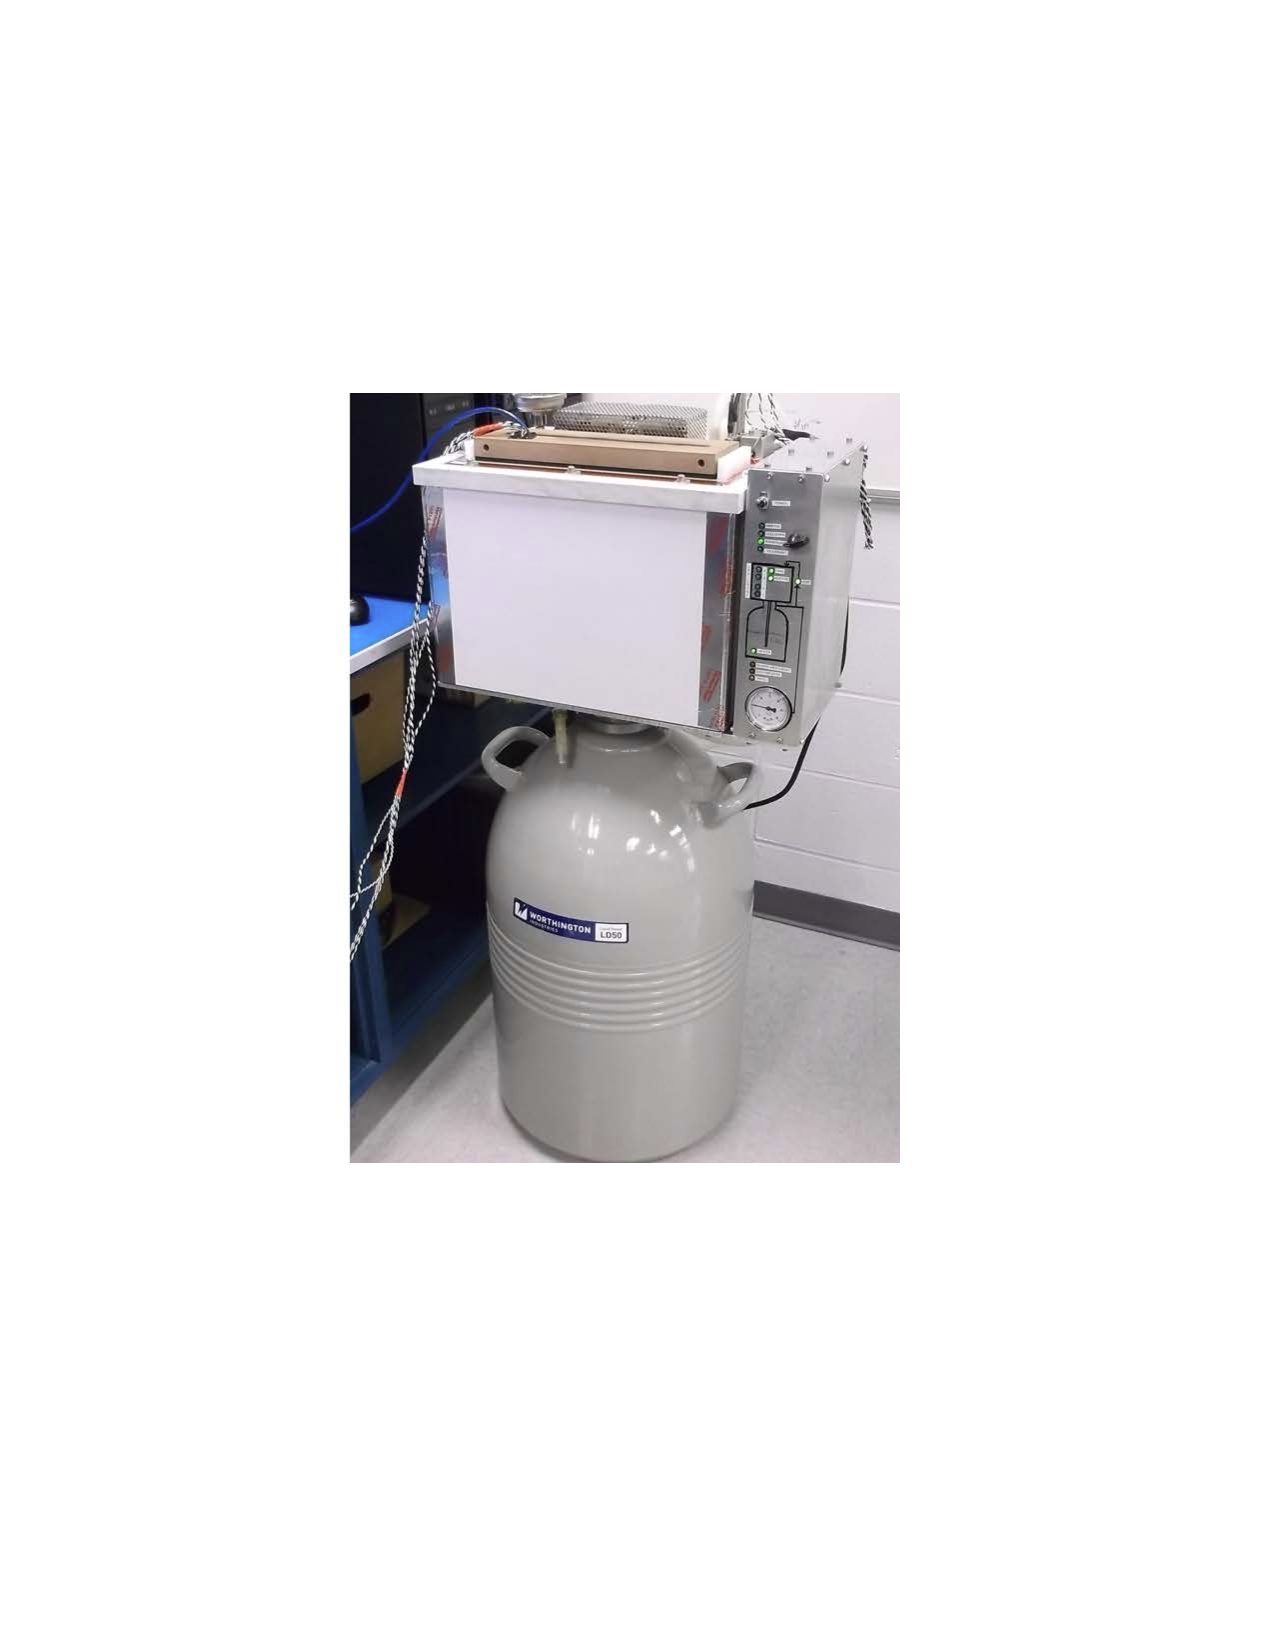
\includegraphics[width=0.5\textwidth]{figures/CTS.pdf}
\end{center}
%\end{minipage}
\caption{Cryogenic Test System.}
\label{fig:cts}
\end{figure}


\subsection{BNL Test System }
\label{sec:2.2}

Describe BNL test setup including the test boards.

\subsection{Fermilab Cryocooler Test System }
\label{sec:2.3}
%%%%%%%%%%%%%%%%%%%%%%%%%%%%%%%%%%%%%%%%%%%%%%%%%%%%%%%
%(Christian) Fermilab test setup including the test boards
%%%%%%%%%%%%%%%%%%%%%%%%%%%%%%%%%%%%%%%%%%%%%%%%%%%%%%%
\begin{figure}[htb]
\centering
%\begin{minipage}[b]{1.0\textwidth}
\begin{center}
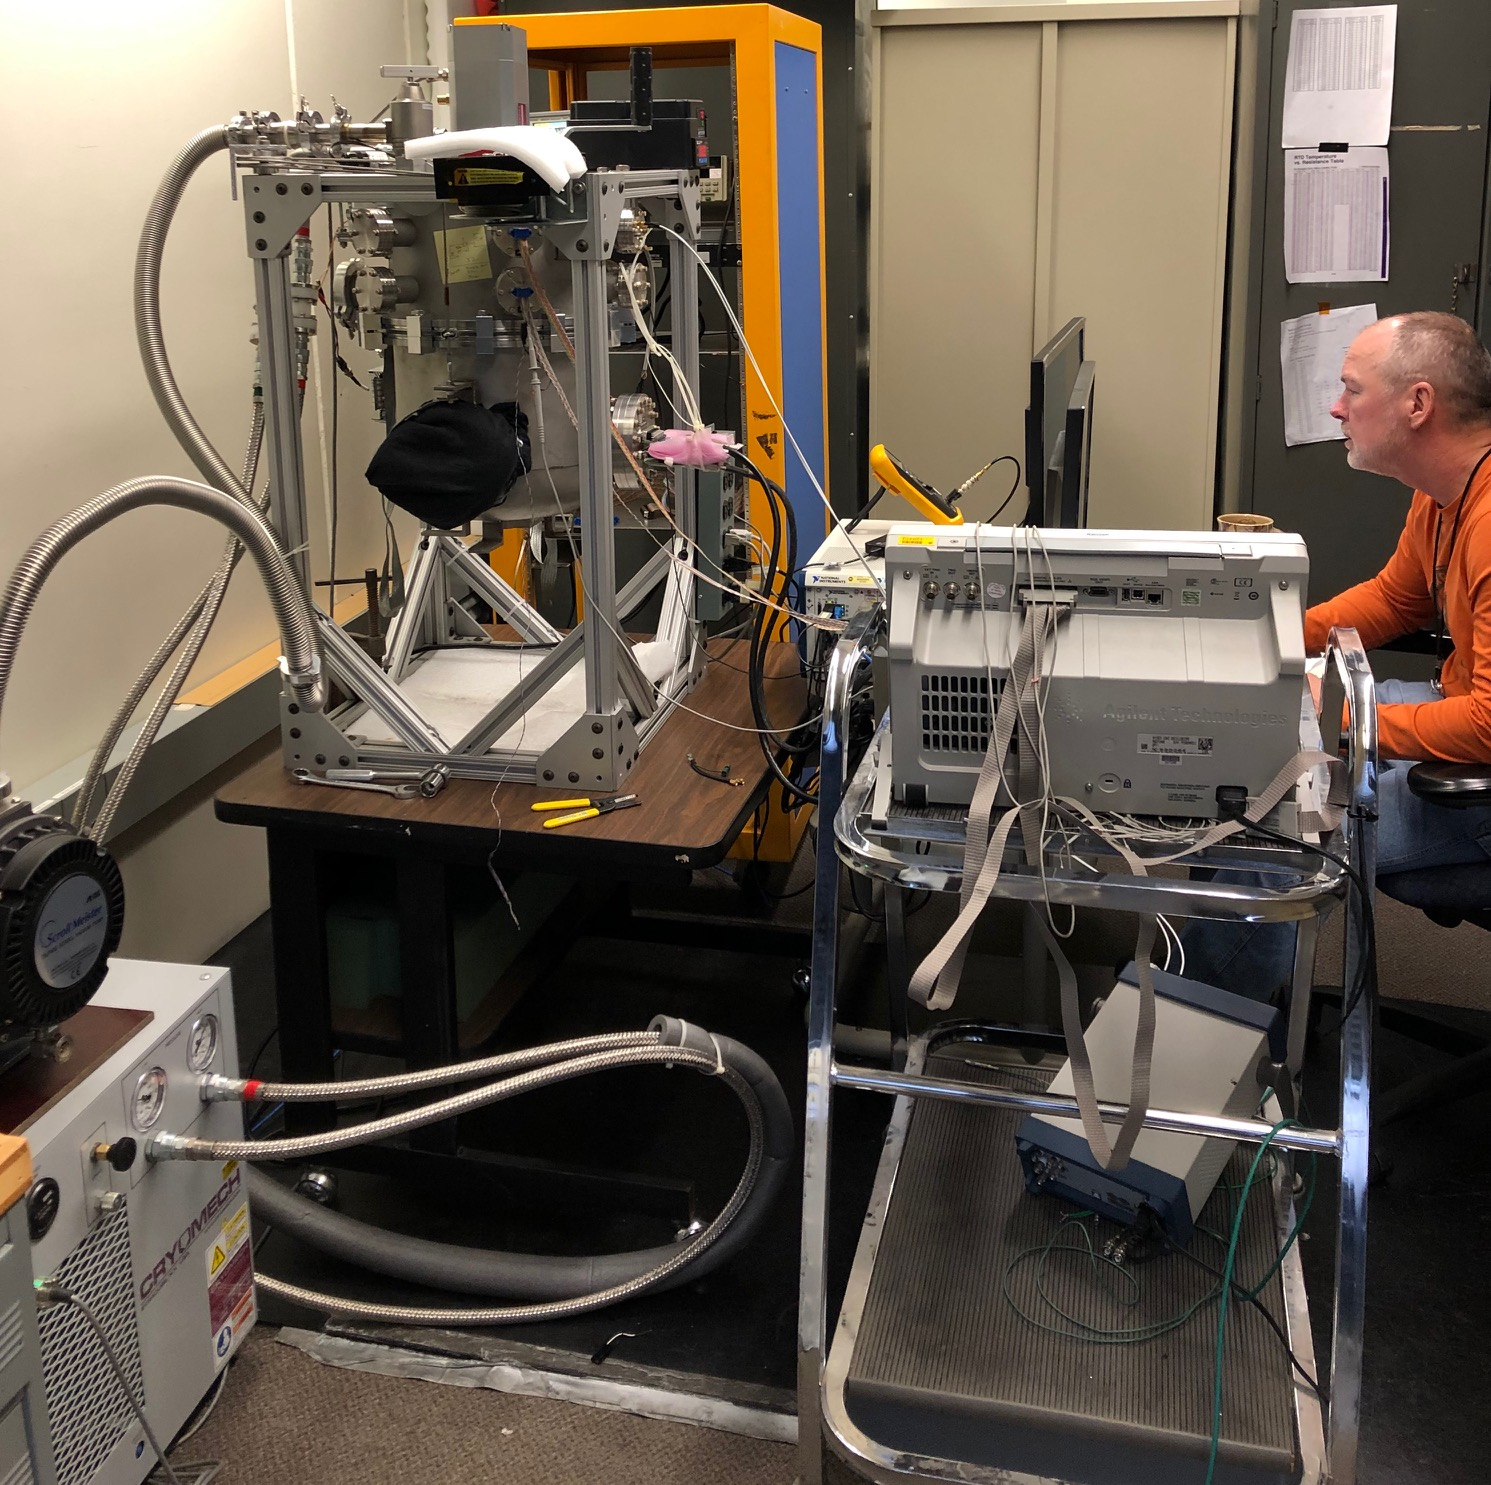
\includegraphics[width=0.95\textwidth]{figures/cryotestsystem.jpg}
\end{center}
%\end{minipage}
\caption{Fermilab Cryocooler Test System.}
\label{fig:cryocoolertestsystem}
\end{figure}

The Fermilab Cryocooler Test System, see Figure~\ref{fig:cryocoolertestsystem}, consists of a vacuum vessel and a cryogenic refrigerator. The cryogenic refrigerator is a Cryomech PT-60.  It is a closed-loop cryocooler consisting of a helium compressor (located next to the vacuum vessel) and a cold head (located on top of the vacuum vessel).  The cryocooler cools a copper cold-plate inside the vacuum vessel to a minimum of 60 K.  A 100 ohm platinum RTD and a 75 Watt heater are mounted on the cold-plate.  A temperature controller cycles the heater on and off to achieve the set-point temperature.  Any temperature between 60 and 250 K can be set.
The vacuum vessel has 2 large penetrations and 12 small penetrations that can be used in device testing.  Typically, one of the large penetrations is used as an inspection port and the other as a feedthrough for ribbon cables.  The small ports allow for a variety of other signal feedthroughs.  

Two printed circuit boards are used in ASIC testing, a ``cold board,'' which is screwed onto the cold-plate and includes a large unmasked copper thermal contact area, and a ``warm board'' which is mounted as a mezzanine board on the cold-board.  RTDs are placed on both the cold board and the warm board.  The temperature on the warm board is typically 100 K higher than than the temperature on the cold board.  If the cryocooler is regulated to hold the cold-board at LN$_2$ temperature, then the temperature on the warm board is $\sim-96^{\circ}$C, which is warm enough for most COTS components to operate properly.

The cold board used in tests of ColdADC includes a single bare chip, wire bonded to the printed circuit board.  An 80-pin header carries digital I/O and three of the four bias voltages (VDDIO and both digital voltages) between the cold board and the warm board.  A 60 pin header carries the analog bias voltage and all analog signals with the exception of the analog inputs to the ColdADC.  Jumpers allow the analog inputs to be grounded or connected to an external sources using cables.  The only other parts on the cold board are bypass capacitors (selected for cryogenic use) and test points.

The warm board includes connectors that mate to the cold board connectors, a 52-pin header used for a cable connection to an National Instruments (NI) FPGA module, single ended to differential converters used for the 64 and 2 MHz clock signals, differential to single ended converters for the LVDS output signals, level shifters for the CMOS I/O signals, passive components, buffer amplifiers, and SMA connectors for the analog outputs, SMA connectors for the ADC test inputs, and 9-pin D connectors for cable connections to NI power supplies that provide source-measure functionality (used for chip power and for providing or measuring analog I/O signals such as reference voltages).

Test software was written using National Instruments LabView and run on a single-crate PXIe system consisting of a controller, an NI 6583 FPGA unit, and 5 power supply modules.  A Keysight 33500B waveform generator was used to provide input signals.  Analog measurements were made using an oscilloscope and a DVM as well as with the NI modules.


\subsection{LBNL Test System }
\label{sec:2.4}

%%%%%%%%%%%%%%%%%%%%%%%%%%%%%%%%%%%%%%%%%%%%%%%%%%%%%%%
% Lin and Prakash - LBL test setup
%%%%%%%%%%%%%%%%%%%%%%%%%%%%%%%%%%%%%%%%%%%%%%%%%%%%%%%

\subsubsection {LBNL mother board}

A single board solution was developed by LBNL to test the ColdADC. The mother board accommodates one ColdADC bare die, wire bonded to the board. The mother board is divided into ``cold" and ``warm" sections with an empty strip of PCB in between to clamp the board to CTS. The ColdADC, extremely low noise LDO's which supply four different VDDs to the ColdADC are present in the ``cold section" of the mother board. Power supply distribution circuitry, Spartna 6 FPGA, LDO's for the FPGA, 80MHz oscillator for clocking the FPGA, external unity buffers and 12 bit ADCs to digitize the monitor signals from the ColdADC and 40 pin standard header to connect the Raspberry PI are in the ``warm section" of the mother board. Analog inputs to the ColdADC are supplied by 16 edge-mount SMA connectors. There are two additional edge-mount SMA connectors to supply test inputs directly to the ADC-core. Eight-pin standard header connector is available if there is a need to bypass the ColdADC LDOs and supply external VDDs directly to the ASIC.

Although the mother board is very successful, there are three minor limitations: Due to small block-ram size of the FPGA the ADC data cannot be streamed continuously to the Raspberry PI this makes the calibration and linearity calculation of the ColdADC a time consuming process. Secondly, this version of the mother board is a Chip-On-Board (COB) version, this makes testing more than one ASIC very difficult, replacing an ASIC essentially means destroying the current chip and mount a new chip. Finally, the analog inputs to the ColdADC can only be single ended. Due to the lack of space only 16 SMA connectors were mounted on the board.  

A new three board solution was developed to overcome these three limitations. Version 2 LBNL test setup consists of a motherboard, a daughter card and an FPGA mezzanine board. The daughter card can either designed to have bare die or a packaged chip. A modular approach was taken to design the new test setup. The same test setup can be used for ColdADC V2 chip just by minor re-designing the COB daughter card. The V2 LBNL test setup is shown in Figure \ref{fig:v2_board}. This test board, just like the previous version has ``cold section" and ``warm section". The COB daughter card and the LDOs are at the bottom, in the ``cold" section of the board. The power distribution circuitry, FPGA mezzanine board, and the Raspberry PI are in the ``warm" section of the board. Four 8-pin Samtec 5.00 mm 50 Ohm Ganged Micro-Miniature RF Jack connectors are used to drive external differential or single ended analog inputs to the ColdADC.  

\begin{figure}[h!]
\centering
  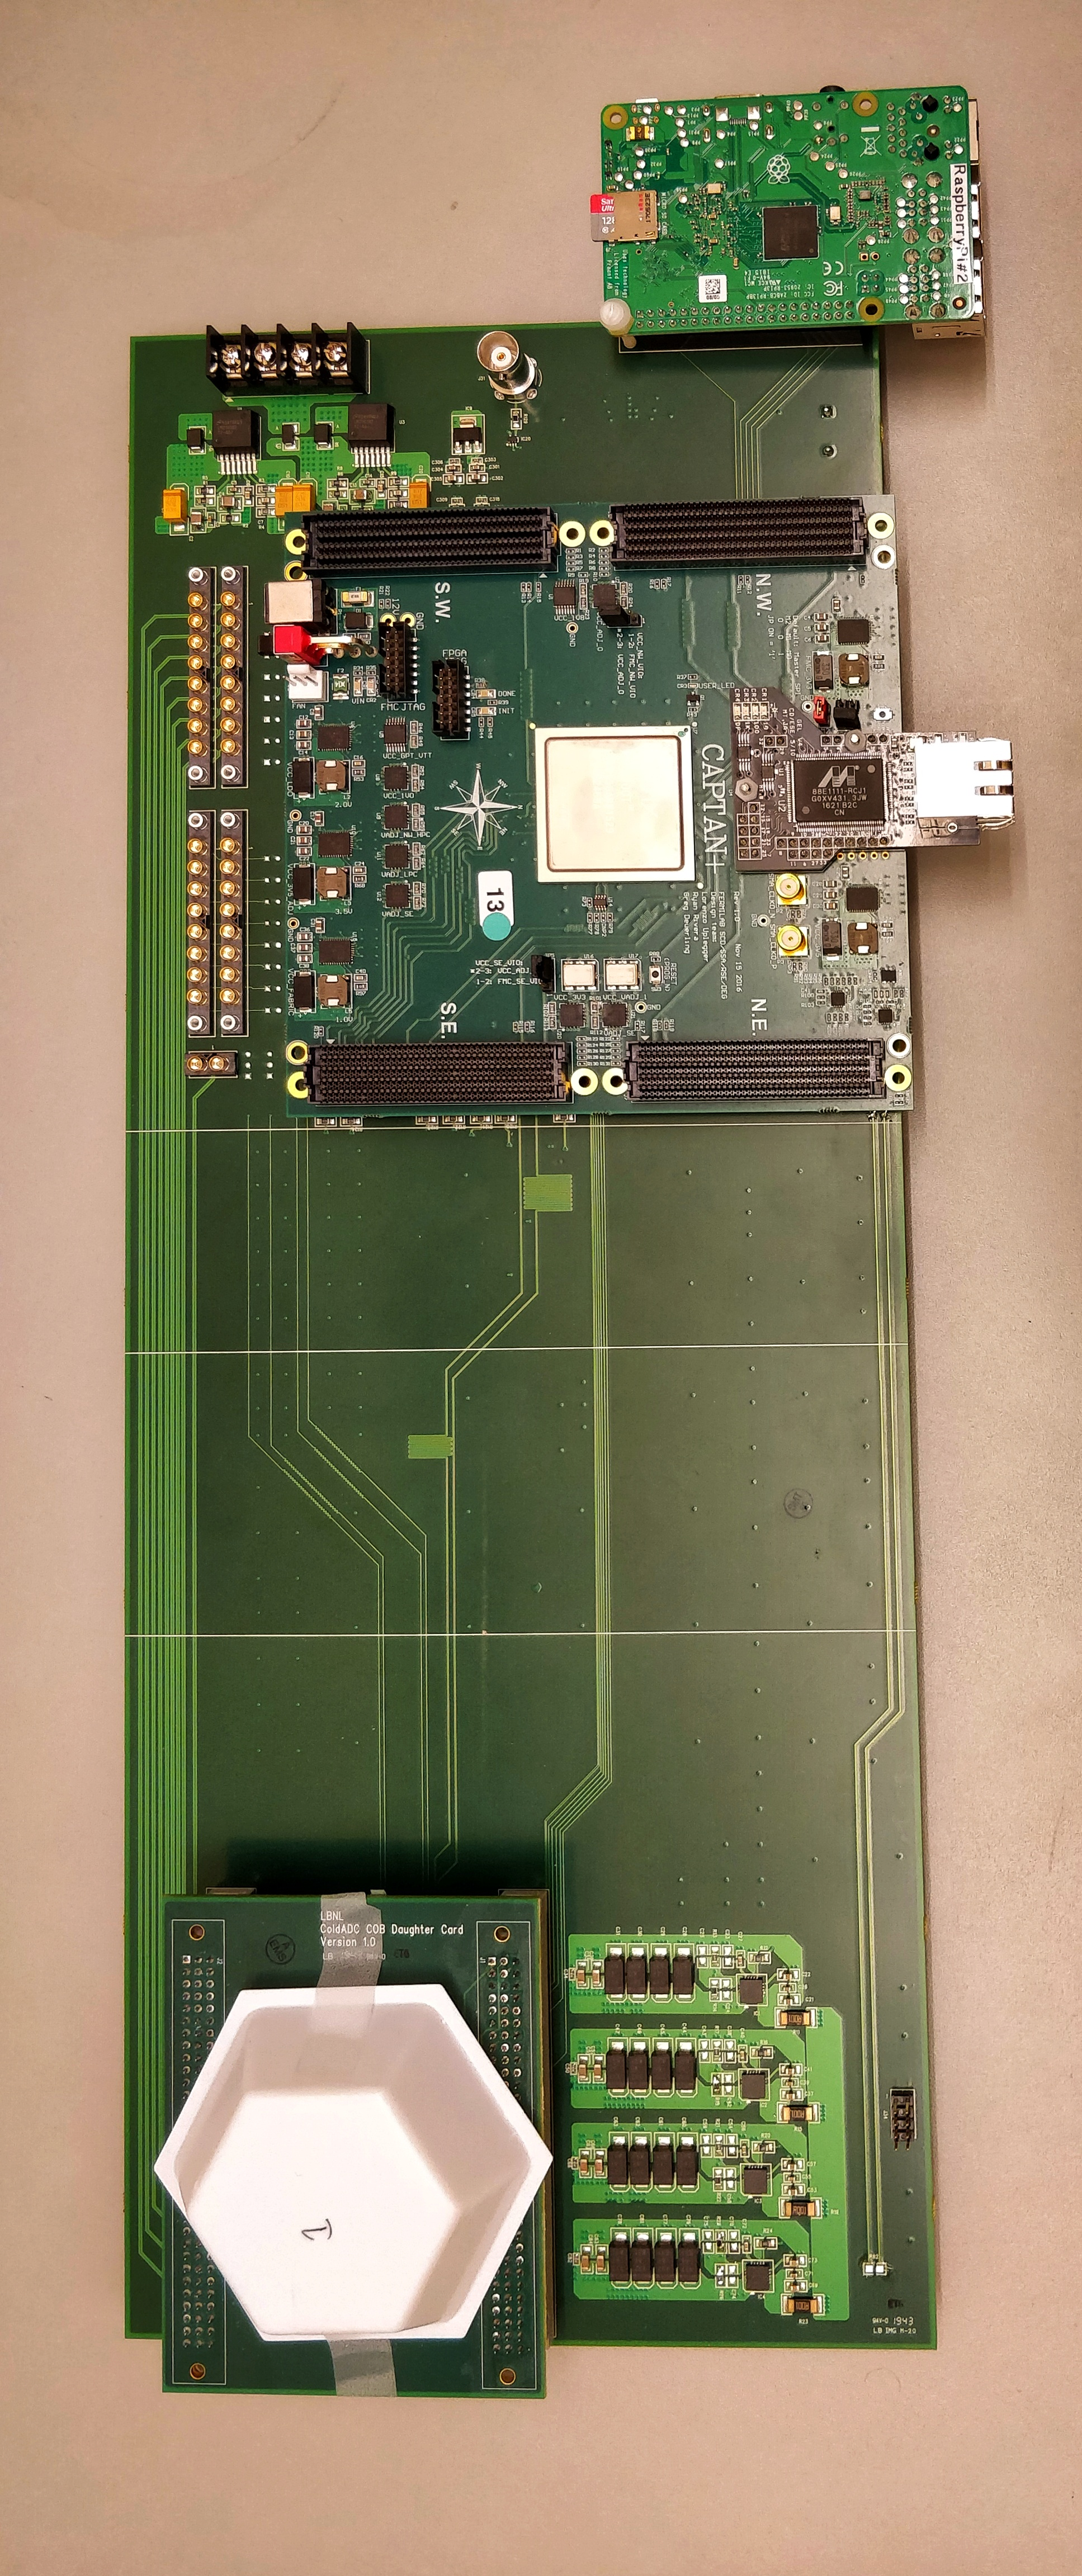
\includegraphics[width=0.3\linewidth]{figures/prakash_fig/v2_board.jpeg}
  \caption[LBNL ColdADC Testboard]{Version 2 LBNL ColdADC Testboard}
  \label{fig:v2_board}
\end{figure}




%%%%%%%%%%%%%%%%%%%%%%%%%%%%%%%%%%%%%%%%%%%%%%%%%%%
\newpage
\section{Functional Testing }
\label{sec:3}

COLDADC is highly programmable.  Many circuit blocks can be bypassed and two versions of a number of circuit blocks are included to mitigate the risk that one might fail.  Testing at Fermilab concentrated on verifying the functionality of all of the circuit blocks.  Three design errors were revealed and a number of documentation errors were corrected.  The table below summarizes the tests.
 
 \begin{table}[h]
\centering
\begin{tabular}{|c|c|}
\hline
\textbf{ Test/Circuit} & Result  \\ \hline \hline
Power on &  No shorts \\ \hline
I2C & Works as designed (registers can be written and read) \\ \hline
Reset & Works as designed (registers are set to default values) \\ \hline
UART & Works as designed \\ \hline
LVDS I/O & Works as designed (output amplitude controlled as designed) \\ \hline
Clock Generation & 16 MHz clock verified \\ \hline
Data Formatter & Works as designed \\ \hline
Band Gap Reference & Works $\sim$as designed at room temperature, but fails when cold. \\ 
 & Problem traced to a design error (inclusion of the wrong \\ 
 &  OP Amp in the current source DAC); works as designed \\ 
 &  with elevated VDDA2P5 (needs 2.7V at 77K) \\ \hline
 CMOS Reference & Works as designed \\ \hline
 Automatic Calibration & Fails.  Calibration can be done by using control \\ 
  & registers to force the sequence of steps required \\ 
   & and doing arithmetic off-chip.\\ 
    & Eventually we noticed that when automatic calibration is \\ 
     & attempted, the low order bytes of W0 and W2 for every \\ 
      & ``calibrated'' stage are equal. Simulation verified that  \\ 
       & this is due to a timing error storing W0 and W2. \\ \hline
 ADC Correction Logic & Works as designed (loaded fake comparator output \\ 
  & values; resulting ADC output is as expected). \\ \hline
Pipeline ADC & Linear ramp yields close to linear output; \\ 
 & deviation from linear at extremes of ramp; \\ 
  & no significant deviation from linear when cold. \\ \hline
Input buffers & Significant non-linearity observed. \\ 
 & Problem traced to circuit naming confusion that resulted \\ 
 & in level shifters being omitted from input buffers. \\
 & Buffers operate $\sim$as designed with elevated VDDD1P2 \\ \hline
 Sample and Hold and MUX & Require elevated VDDD1P2 because \\ 
 & inputs come through input buffers. \\ \hline
\end{tabular}
\caption{Functional Testing.}
\label{tab:Functionality}
\end{table}

	
%%%%%%%%%%%%%%%%%%%%%%%%%%%%%%%%%%%%%%%%%%%%%%%%%%%
\newpage
\section{Performance Results}
\label{sec:4.}

%%%%%%%%%%%%%%%%%%%%%%%%%%%%%%%%%%%%%%%%%%%%%%%%%%%%%%%
%Performance Results 
%%%%%%%%%%%%%%%%%%%%%%%%%%%%%%%%%%%%%%%%%%%%%%%%%%%%%%%

The ColdADC is designed with many redundancies to mitigate single point of failure. During functional testing, a number of 
problems were identified. Forunately, none of the problems prevented the ColdADC from achieving a performance that meets 
the key DUNE requirements. In this section we will show the performance results (already summarized 
in Table~\ref{tab:coldadc_specs}) with the ASIC in the nominal configuration, the same configuration that we will 
use for the system-level integration tests at CERN on APA\#7 in the Coldbox and the ICEBERG teststand at Fermilab.


\subsection{Noise}
\label{sec:4.1}

%%%%%%%%%%%%%%%%%%%%%%%%%%%%%%%%%%%%%%%%%%%%%%%%%%%%%%%
%(GAO) Discuss noise performance
%%%%%%%%%%%%%%%%%%%%%%%%%%%%%%%%%%%%%%%%%%%%%%%%%%%%%%%
The key performance metric for the ColdADC is its noise performance, as it directly impacts the 
sensitivity of the experiment. The design goal for the ColdADC was for its internal noise to be well 
below the noise of the LArASIC, so the LArASIC would dominate the overall noise of the system. 
This has been achieved as the ADC met its goal of 200 $\mu$V-rms noise at LN$_2$ temperature. 
Detailed measurements of the ASIC and system noise in different conditions follow.

\subsubsection{ColdADC Only}
The noise distribution for 16-channels from one ColdADC chip with the input floating are shown in Figure~\ref{fig:qc_noisewarm} (RT) and Figure~\ref{fig:qc_noisecold} (LN$_2$). The results are given in full 16-bit ADC output. The average noise is 6.7 LSB (302 $\mu$V-rms) at warm and 4.2 LSB (189 $\mu$V-rms) in LN$_2$, in 16-bit. The measurement is done with ColdADC configured after calibration, VDDA2P5/VDDD2P5=2.5 V, VDDD1P2=2.0 V, VDDIO=2.25 V, SDC bypassed. Separate study has shown that SDC noise is negligible. 
\begin{figure}[h!]
\centering
  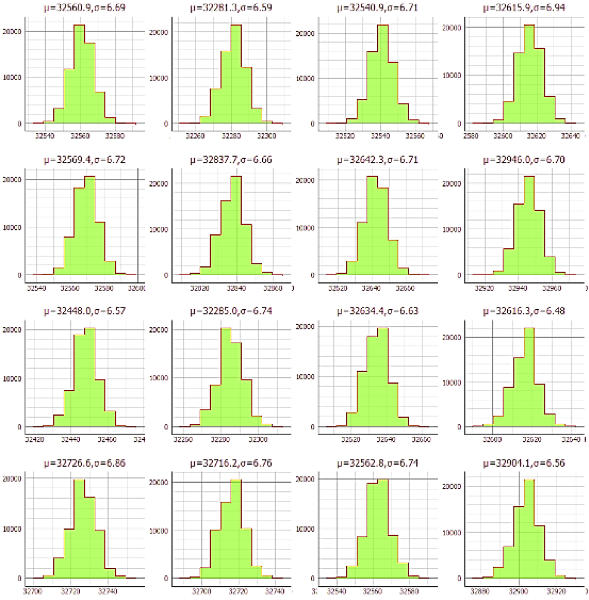
\includegraphics[width=0.8\linewidth]{figures/qc_noisewarm.png}
  \caption{Noise distribution (16-bit) of 16 input channels at room temperature.}
  \label{fig:qc_noisewarm}
\end{figure}
\begin{figure}[h!]
\centering
  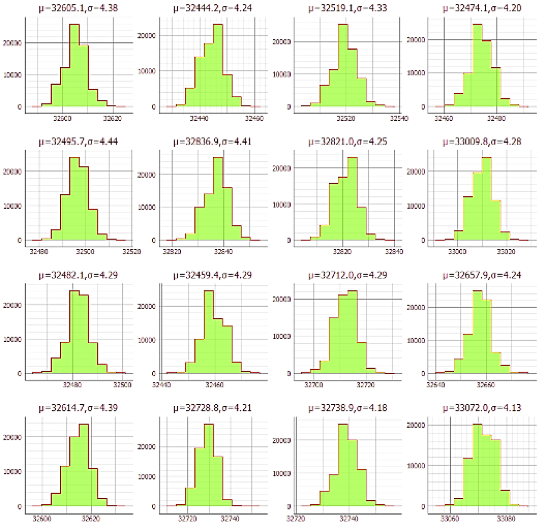
\includegraphics[width=0.8\linewidth]{figures/qc_noisecold.png}
  \caption{Noise distribution (16-bit) of 16 input channels at LN$_2$ temperature.}
  \label{fig:qc_noisecold}
\end{figure}

\subsubsection{LArASIC + ColdADC}
To evaluate the combined noise of LArASIC and ColdADC, 150pF mica capacitor is added to the LArASIC input 
to simulate the capacitance of the detector sense wire. 
Noise characterization is made at both room and LN2 temperatures, as shown in Figure~\ref{fig:noise_fullchain}.  
The quantization noise of 12-bit ADC is negligible when LArASIC gain is set to 7.8 mV/fC or higher.
With a shaping time $>$ 2 $\mu$s, the ENC noise is below 630 e$^-$ at RT and $<$ 500 e$^-$ at LN$_2$ temperature.
\begin{figure}[h!]
\centering
  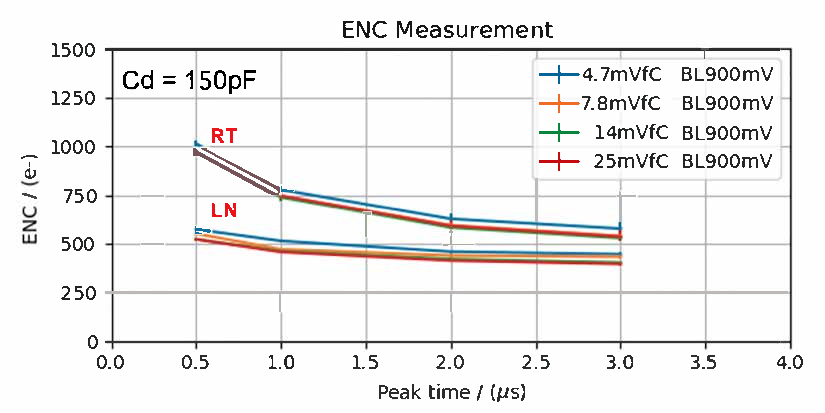
\includegraphics[width=0.8\linewidth]{figures/noise_fullchain.pdf}
  \caption{LArASIC + ColdADC (12-bit mode) noise as a function of shaping time at RT and LN$_2$ temperatures.}
  \label{fig:noise_fullchain}
\end{figure}

The noise dependence on the input capacitance is also studied. In this setup, each input LArASIC channel has
a different capacitor with value that ranges from 22 pF to 150 pF. The input capacitance dependence result in 
LN$_2$ is shown in Figure~\ref{fig:noise_capacitance} . The four different curves correspond 
to different values of LArASIC shaping time. 
The noise performance comparison between ColdADC BGR and CMOS reference, and comparison between 
SDC and bypassing SDC show no significant difference.
The ENC noise performance for the LArASIC + ColdADC setup has better noise perforamnce compared to 
MicroBooNE, ProtoDUNE, and SBND cold electronics (see results in the Appendix).
\begin{figure}[h!]
\centering
  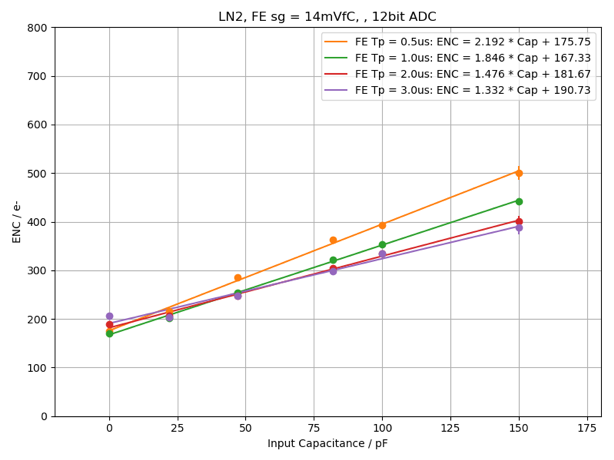
\includegraphics[width=0.8\linewidth]{figures/noise_capacitance.png}
  \caption{ENC vs. input capacitance at LN$_2$ temperature. LArASIC is configured with a gain setting of
14 mV/fC, ColdADC output is trucated to 12-bit. The four curves corresponds to (from to to bottom) 0.5, 
1.0, 2.0, and 3.0 $\mu$s shaping time.} 
  \label{fig:noise_capacitance}
\end{figure}

The DUNE requirement calls for a 12-bit ADC. The nominal plan is to trucate 16-bit ColdADC output down to 
12-bit. Given the low noise of the ColdADC, we explore the feasibility of outputing more than 12-bit.
Earlier Figure~\ref{fig:noise_fullchain} demonstrates that when LArASIC gain is set to 7.8 mV/fc or higher, 
the quantitization noise of 12-bit ADC is negligible. Figure~\ref{fig:noise_quant150pf} 
shows the ENC as a function of shaping time for 16, 14, and 12 bit ADC output with input LArASIC capacitance
of 150 pF. Figure~\ref{fig:noise_quantfloat} shows the ENC with LArASIC input floating. With the 
current noise performance, the quantization noise is negligible at 14-bit output even with the lowest LArASIC gain setting of 4.7 mV/fC.
\begin{figure}[h!]
\centering
  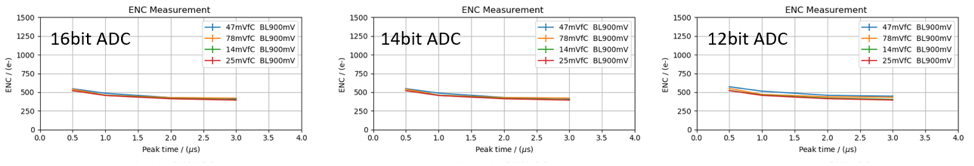
\includegraphics[width=1.0\linewidth]{figures/noise_quant150pf.png}
  \caption{ENC vs. Shaping Time at LN$_2$ temperature. Input capacitance is 150 pF. Different curves 
correspond to gain setting of (top to bottom) 4.7, 7.8, 14, 25 mV/fC.}
  \label{fig:noise_quant150pf}
\end{figure}
\begin{figure}[h!]
\centering
  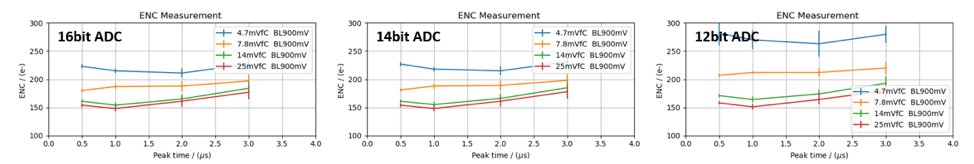
\includegraphics[width=1.0\linewidth]{figures/noise_quantfloat.png}
  \caption{ENC vs. Shaping Time at LN$_2$ temperature. Input floating. Different curves correspond to 
gain settings of (top to bottom) 4.7, 7.8, 14, 25 mV/fC.}
  \label{fig:noise_quantfloat}
\end{figure}





\clearpage
\newpage
\subsection{Static Linearity (DNL,INL)}
\label{sec:4.2}

%%%%%%%%%%%%%%%%%%%%%%%%%%%%%%%%%%%%%%%%%%%%%%%%%%%%%%%
% Static Linearity (INL, DNL) 
%%%%%%%%%%%%%%%%%%%%%%%%%%%%%%%%%%%%%%%%%%%%%%%%%%%%%%%

To evaluate the Differential Nonlinearity (DNL) and Integral Nonlinearity (INL) of the ColdADC, a sine wave is applied to the single-ended input of the ColdADC. The resulting ADC code density histograms are used to extract DNL and INL. Some representative distributions at LN$_2$ temperature are shown in Figure~\ref{fig:adc_inldnl}.

\begin{figure}[htb]
\centering
%\begin{minipage}[b]{1.0\textwidth}                                                                                                                    
\begin{center}
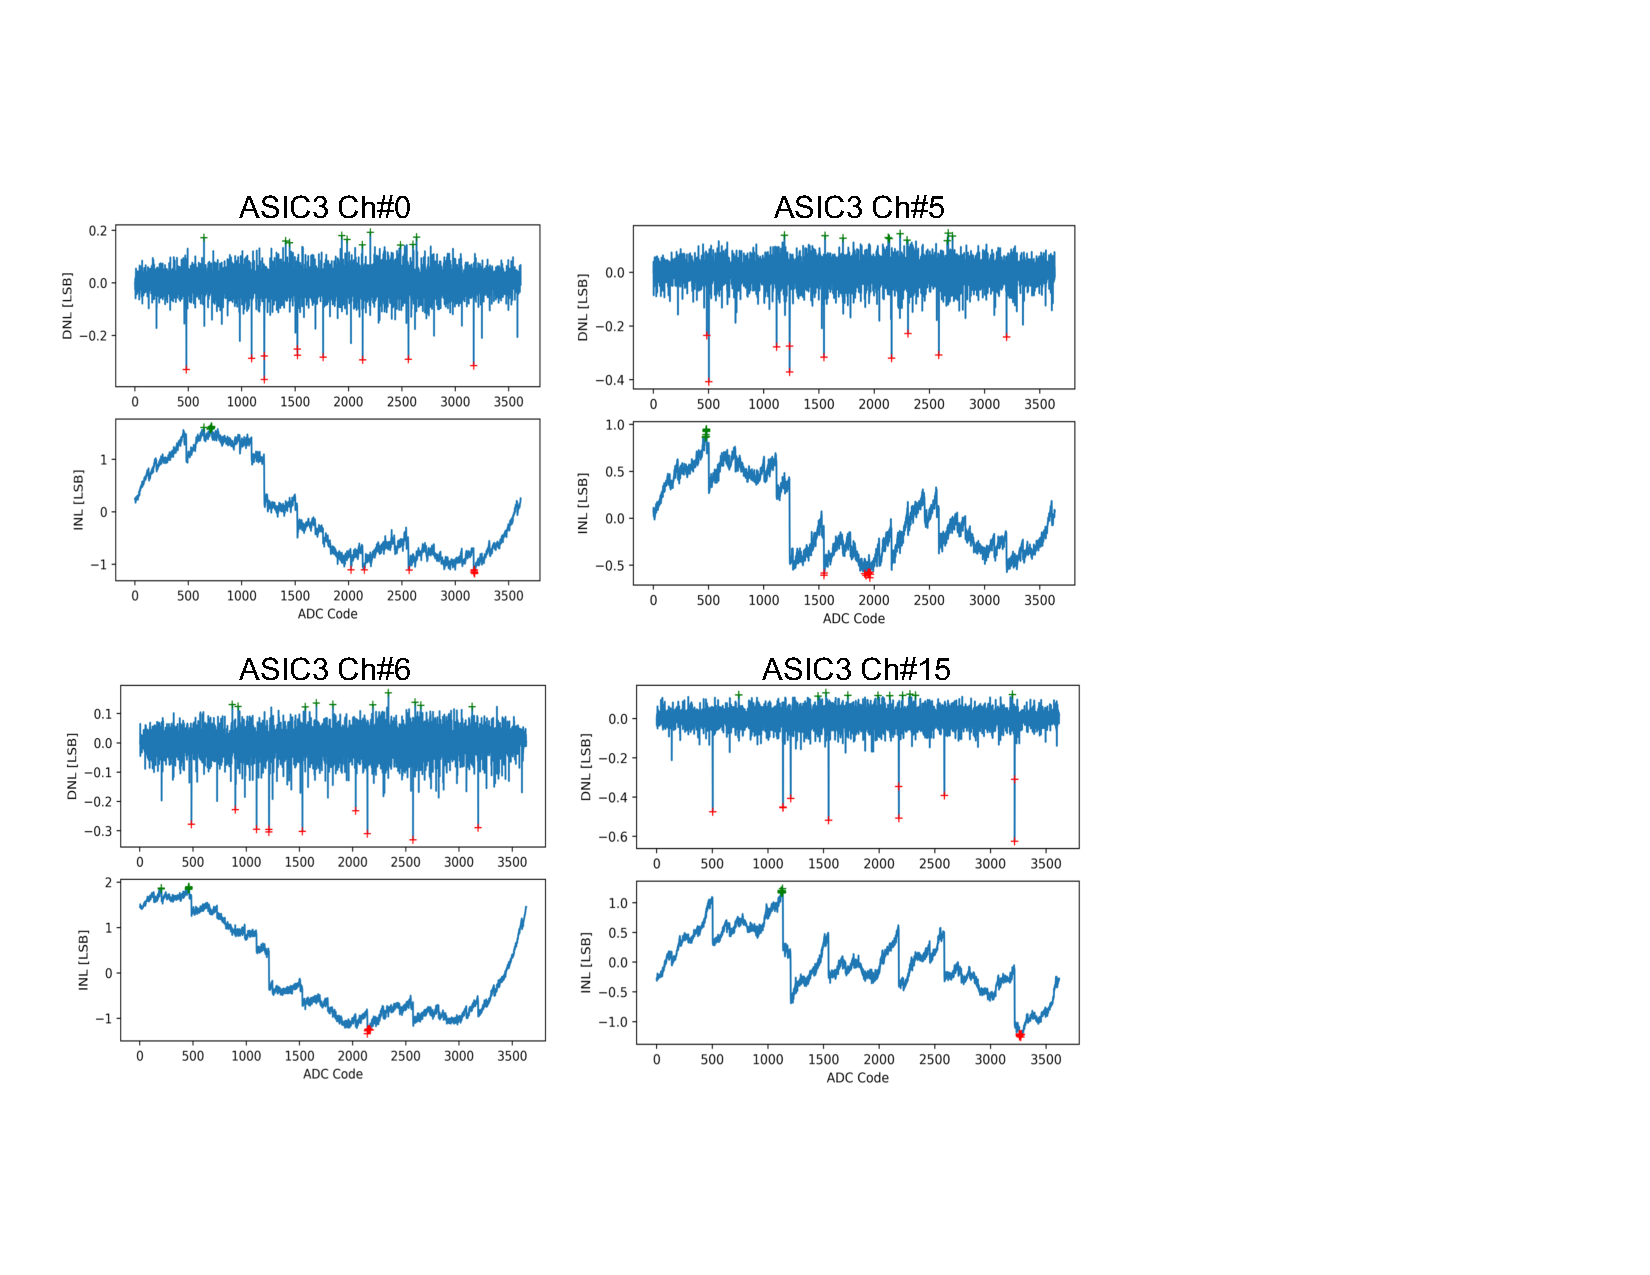
\includegraphics[width=1.0\textwidth]{figures/ColdADC_StaticLinearity.pdf}
\end{center}
%\end{minipage}                                                                                                                                        
\caption{DNL and INL for a few representative channels on ColdADC ASIC\#3 at LN$_2$ temperature.}
\label{fig:adc_inldnl}
\end{figure}

The typical DNL vs. ADC code has a narrow band between $\pm 0.1$ (12-bit) but exibits large negative spikes. The source of the spikes are attributed to residual nonlinearity from the MUX-SHA stage (to be discussed in Section~\ref{sec:5.4}). The DNL extremas, dominated by the spikes, across all channels are typicall between $+0.2$ to $-0.5$ LSB. The average INL extremas are from $+1.2$ to $-1.1$ LSB.



\subsection{Dynamic Linearity (ENOB, SNDR)}
\label{sec:4.3}

%%%%%%%%%%%%%%%%%%%%%%%%%%%%%%%%%%%%%%%%%%%%%%%%%%%%%%%
% Dynamic Linearity
%%%%%%%%%%%%%%%%%%%%%%%%%%%%%%%%%%%%%%%%%%%%%%%%%%%%%%%

The dynamic performance of an ADC is determined by the effective number of bits (ENOB). Figure~\ref{fig:coldadc_fft} shows the Fast-Fourier Transform (FFT) from one of the ADC channels.  The ENOB across ADC channels at LN$_2$ temperature is generally fairly uniform with a mean value of 10.6 bits and a spread of about 0.3 bits. 
\begin{figure}[htb]
\centering
%\begin{minipage}[b]{1.0\textwidth}
\begin{center}
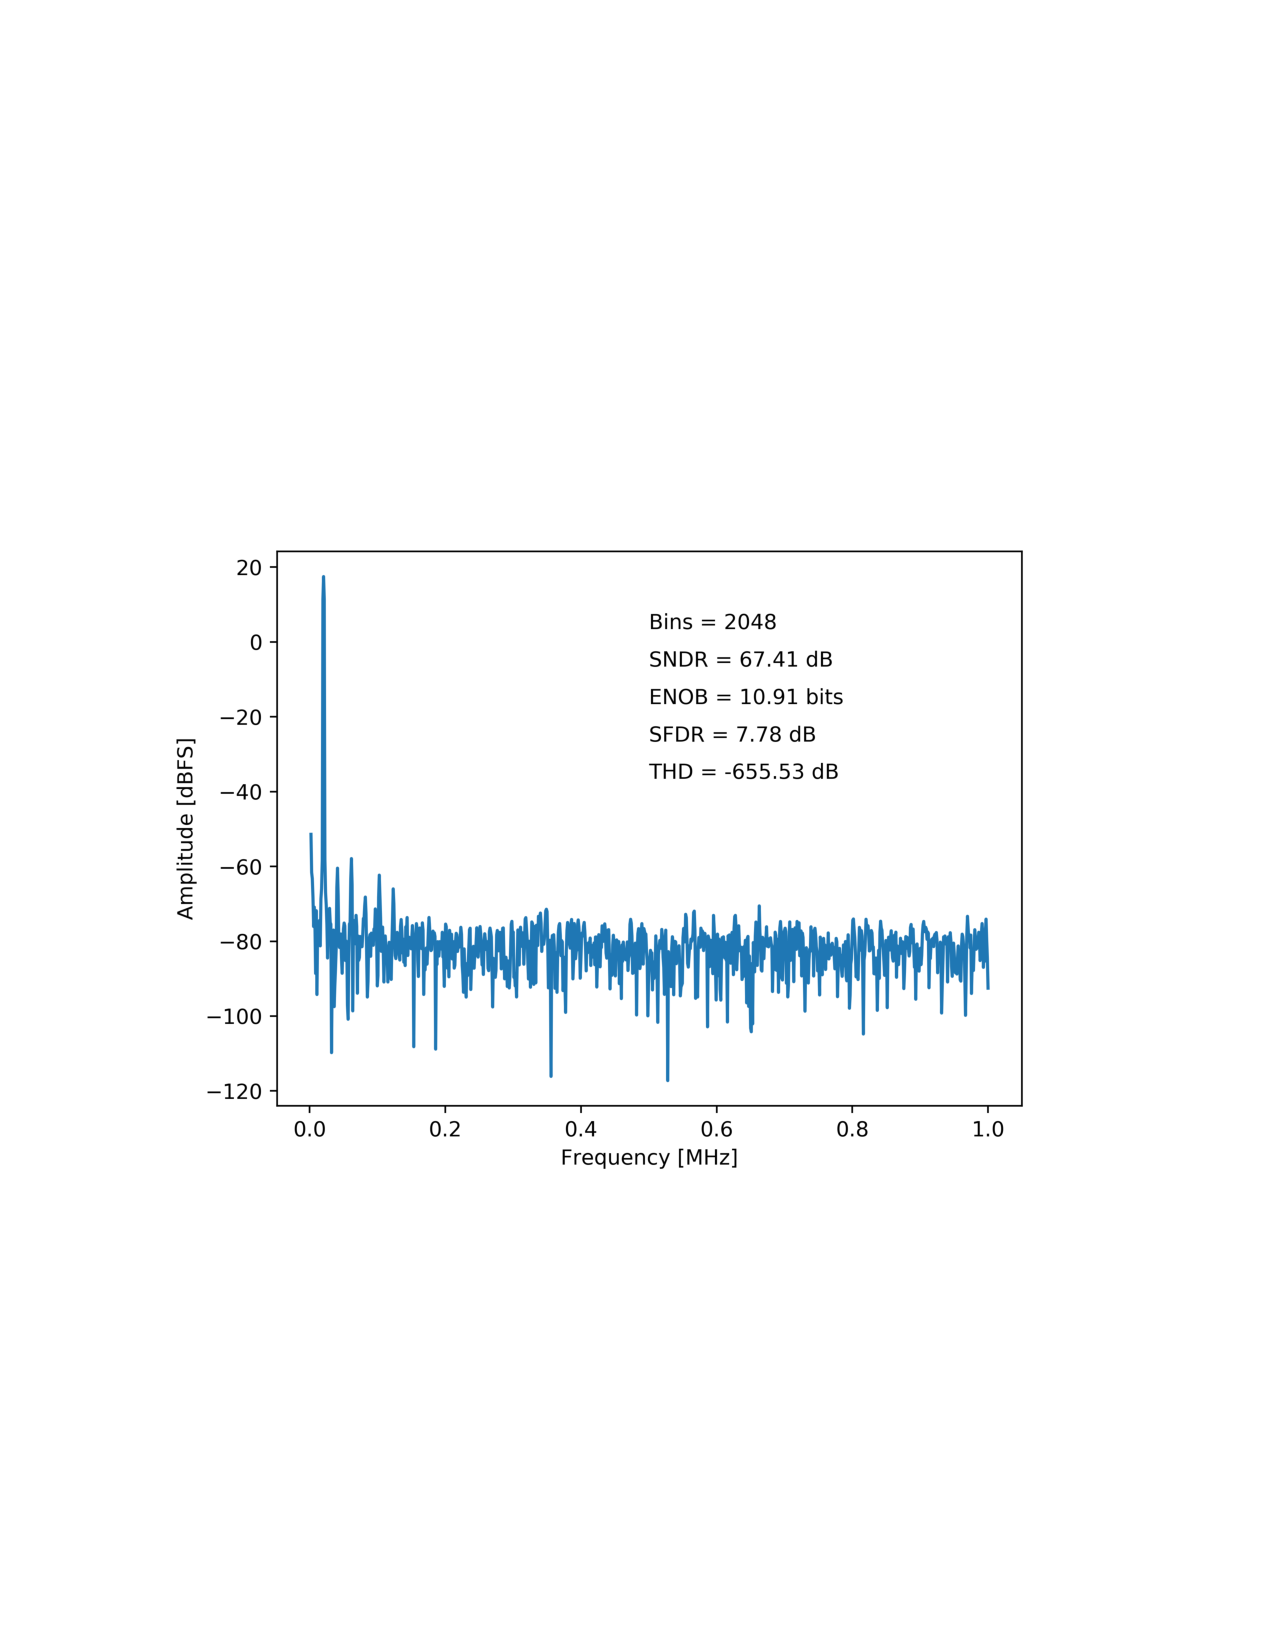
\includegraphics[width=0.7\textwidth]{figures/fft_Sinusoid_20KHz_SE-SHA-ADC0_NomVREFPN_2M_v1.pdf}
\end{center}
%\end{minipage}
\caption{FFT.}
\label{fig:coldadc_fft}
\end{figure}




\clearpage
\newpage
\subsection{Linearity Measurement using LArASIC Calibration Pulser}
\label{sec:4.4}
%%%%%%%%%%%%%%%%%%%%%%%%%%%%%%%%%%%%%%%%%%%%%%%%%%%%%%%
%(GAO) Calibration pulser
%%%%%%%%%%%%%%%%%%%%%%%%%%%%%%%%%%%%%%%%%%%%%%%%%%%%%%%
The LArASIC has an internal 6-bit DAC to generate a voltage step through a charge injection 
capacitor for calibration. Figure~\ref{fig:calibpulse} shows the pulse response of channel 0 at 
room temperature.  LArASIC is configured with 14 mV/fC gain, 2.0 $\mu$s shaping time, 
900mV baseline, output buffer off, DC coupling and 500pA leakage current. ColdADC is configured 
with single-ended input, BGR reference and 16-bit calibrated data. The observed non-linearity of 
0.19\% is dominated by the non-linearity of the 6-bit DAC. The non-linearity of LArASIC and 
ColdADC is expected to be less than 0.1\%.   
\begin{figure}[h!]
\centering
  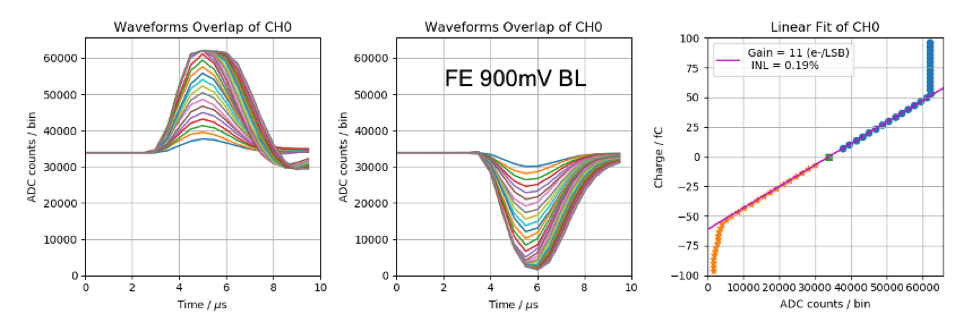
\includegraphics[width=1.0\linewidth]{figures/calibpulse.png}
  \caption{Response of LArASIC + ColdADC to the calibration pulse.}
  \label{fig:calibpulse}
\end{figure}


\clearpage
\newpage
\subsection{Channel Crosstalk }
\label{sec:4.5}
%%%%%%%%%%%%%%%%%%%%%%%%%%%%%%%%%%%%%%%%%%%%%%%%%%%%%%%
%(GAO) Discuss ColdADC Channel Crosstalks
%%%%%%%%%%%%%%%%%%%%%%%%%%%%%%%%%%%%%%%%%%%%%%%%%%%%%%%
The schematic diagram for the input channel crosstalk study is shown in Figure~\ref{fig:xtalk_schematic}. The crosstalk on neighboring channels is
 related to the impedance of the channels. Instead of characterizing the crosstalk for the ColdADC alone, the 
crosstalk from both the LArASIC and ColdADC is measured together in this study. A large calibration charge 
pulse is injected into a specified LArASIC channel, and the responses of the neighboring channels are recorded. A sample crosstalk result at 
room temperature is presented in Figure~\ref{fig:xtalk_RT}. In this case the calibration pulse is injected into CHN0, and the largest crosstalk, close to 1\%, 
is observed on CHN1. The crosstalk on the remaining channels is less than 0.5\%.  When the calibration pulse 
is injected into other channels one by one, it is observed that the next channel within the same ADC core has the largest crosstalk. 
This is an indication that the main contribution of the crosstalk is within the ColdADC itself. At cryogenic temperature, the magnitude of the 
crosstalk is significantly reduced to less than $<$0.5\% across all channels. The results at LN$_2$ is shown in Figure~\ref{fig:xtalk_LN2} with LArASIC configured
for 3$\mu$s shapking time and 14mV/fC gain setting. At 0.5\% level, the crosstalk from LArASIC and ColdADC is neglible compared to the crosstalk 
contribution between sense wires.
\begin{figure}[h!]
\centering
  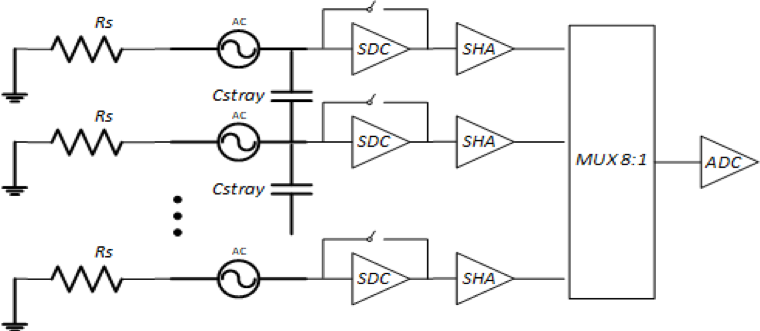
\includegraphics[width=0.7\linewidth]{figures/xtalk_schematic.png}
  \caption{Schematic diagram of the crosstalk measurement.}
  \label{fig:xtalk_schematic}
\end{figure}
\begin{figure}[h!]
\centering
  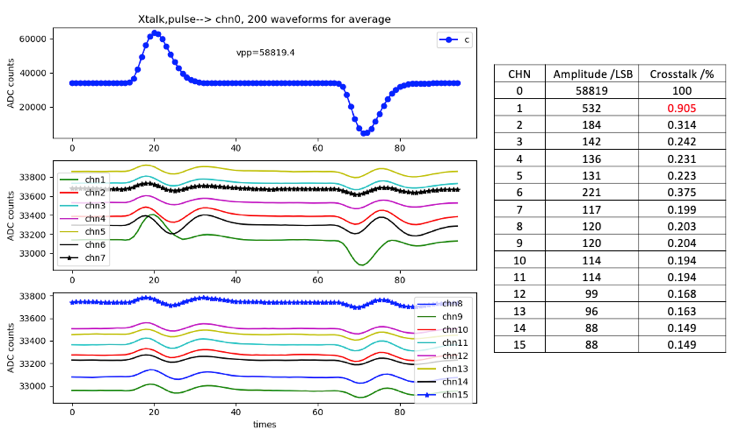
\includegraphics[width=0.7\linewidth]{figures/xtalk_RT.png}
  \caption{Crosstalk waveforms at room temperature. Calibration signal is injected in CHN0. The waveforms of the other 15 channels are shown in the bottom two plots. The amplitude of the cross talk is listed in the Table.}
  \label{fig:xtalk_RT}
\end{figure}
\begin{figure}[h!]
\centering
  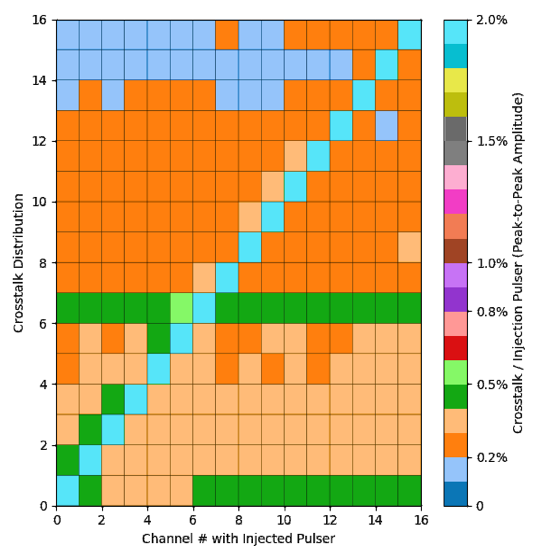
\includegraphics[width=0.7\linewidth]{figures/xtalk_LN2.png}
  \caption{Cross talk distribution at LN$_2$ temperature. The x-axis is the channel number with the injected pulse. The y-axis shows the amplitude of the crosstalk (in \%) for the remaining 15 channels.}
  \label{fig:xtalk_LN2}
\end{figure}


\clearpage
\newpage
\subsection{Power Consumption }
\label{sec:4.6}

%%%%%%%%%%%%%%%%%%%%%%%%%%%%%%%%%%%%%%%%%%%%%%%%%%%%%%%
%(GAO) Discuss ColdADC Power Consumptions
%%%%%%%%%%%%%%%%%%%%%%%%%%%%%%%%%%%%%%%%%%%%%%%%%%%%%%%

The ColdADC is designed with serval power rails with 3 different voltages: VDDA2P5/VDDD2P5 = 2.25 V, VDDIO = 2.25 V, 
and VDDD1P2 = 1.1 V. To achieve good ADC performance, the voltages are elevated to account for IR drop and other
design issues. The  VDDA2P5/VDDD2P5 voltage is raised to 2.5 V when using CMOS reference (2.7 V when using BGR), and 
VDDD1P2 to 2.1 V.
Table~\ref{tab:powerconsumed} shows the measured power consumption under several operating configuration. If ColdADC is powered as 
the design expected, the power consumption is $\approx$ 20 mW per channel with SDC  bypassed (powered down).  If SDC is enabled, 
each channel will consume an extra $\approx$ 6 mW.  When BGR reference is applied, with the elevated VDDA2P5/VDDD2P5 at 2.7 V, the measured
power consumption is $\approx$ 30 mW per channel with SDC powered down.  If CMOS reference is applied, VDDA2P5/VDDD2P5 can be set to 
2.5 V to mitigate the power consumption, which is $\approx$ 26 mW per channel. The issue of raising VDDA2P5/VDDD2P5 to 2.7 V is 
related to the instantiation of an OTA with the wrong input pair polarity (to be discussed in Section~\ref{sec:5.8}).  VDDD1P2 must 
be raised to 2.1 V due to the lack of DC voltage level shifters between 1.2 V and 2.5 V domains (to be discussed in Section~\ref{sec:5.2}). 
Both issues will be addressed in the next version of the ColdADC. We expect power consumption using 
BGR or CMOS references will be roughly the same, and the overall power consumption will be lowered with the new chip.
\begin{table}[h]
\centering
\begin{tabular}{|c|c|c|c|c|c|c|}
\hline
%\textbf{ Temperature  } & \textbf{Value} & \textbf{Result} & \textbf{Note}  \\ \hline \hline
\textbf{Temperature} & RT & RT & RT & LN$_2$ & LN$_2$ & LN$_2$ \\ \hline
\textbf{Reference} & BGR & BGR & CMOS & BGR & BGR & CMOS \\ \hline
\textbf{SDC} & enable & bypassed & bypassed & enable & bypassed & bypassed \\ \hline
\textbf{VDDA2P5/VDDD2P5/ V} & 2.5 &2.5 &2.5 &2.5 &2.5 &2.5 \\ \hline
\textbf{VDD1P2 / V} & 2.1 & 2.1 & 2.1 & 2.1 & 2.1 & 2.1 \\ \hline
\textbf{VDDIO / V} & 2.25 & 2.25 & 2.25 & 2.25 & 2.25 & 2.25  \\ \hline
\textbf{Total Power / mW} & 515 & 418 & 418 & 563 & 513 & 425 \\ \hline
\textbf{Power per Channel / mW} & 32.2 & 26.1 & 26.1 & 35.2 & 32.1 & 26.6 \\ \hline
\end{tabular}
\caption{Power Consumption for ColdADC Chip\#00067}
\label{tab:powerconsumed}
\end{table}  



%%%%%%%%%%%%%%%%%%%%%%%%%%%%%%%%%%%%%%%%%%%%%%%%%%%
\clearpage
\newpage
\section{Issues Identified and Mitigations}
\label{sec:5}

As mentioned earlier, during functional testing of the ColdADC, a number of problems were identified. A series of studies were carried out at the three labs to understand the issues, and come up with solutions to mitigate the problems for the current ASIC, and also fixes for the next version of the design. In this section, we will go through the various issues in more details. 

\subsection{Auto Calibration}
\label{sec:5.1}

%%%%%%%%%%%%%%%%%%%%%%%%%%%%%%%%%%%%%%%%%%%%%%%%%%%
% Autocal
%%%%%%%%%%%%%%%%%%%%%%%%%%%%%%%%%%%%%%%%%%%%%%%%%%%

The linearity of the ADC is primarily determined by the capacitor matching internal to the circuit, and to a lesser extent the performance of the internal amplifiers. To achieve the target specifications, the ADC requires calibration. The calibration in ColdADC can be carried out internal, in a fully automated way, or can be done externally. Unfortunately, while the chip could be fully calibrated externally, with calibration data loaded back onto the chip, the autocal function failed in the prototype. The ADC performance under autocal or external calibration does not differ in any way, so the main issue here is the loss of convenience that autocal promises.

The cause of the auto calibration issue is understood and is mainly due to a miscommunication between ASIC designers. When we developed the digital part of the ColdADC, we decided to partition the blocks such that the blocks calibrate the ADC and compute the corrected digital output would be placed within the ADC cores, and the rest of the digital logic would be aggregated in a third core. This can be seen in Figure~\ref{fig:autocalBlock}. The CAL\_UNIT is the block that performs the calibration and also applies the calibration coefficients (or weights) to the data during normal operation. Each CAL\_UNIT stores the calculated configuration weights to the register file in the CAL\_CORE (which was synthesized separately).
\begin{figure}[h]
\centering
%\begin{minipage}[b]{1.0\textwidth}
\begin{center}
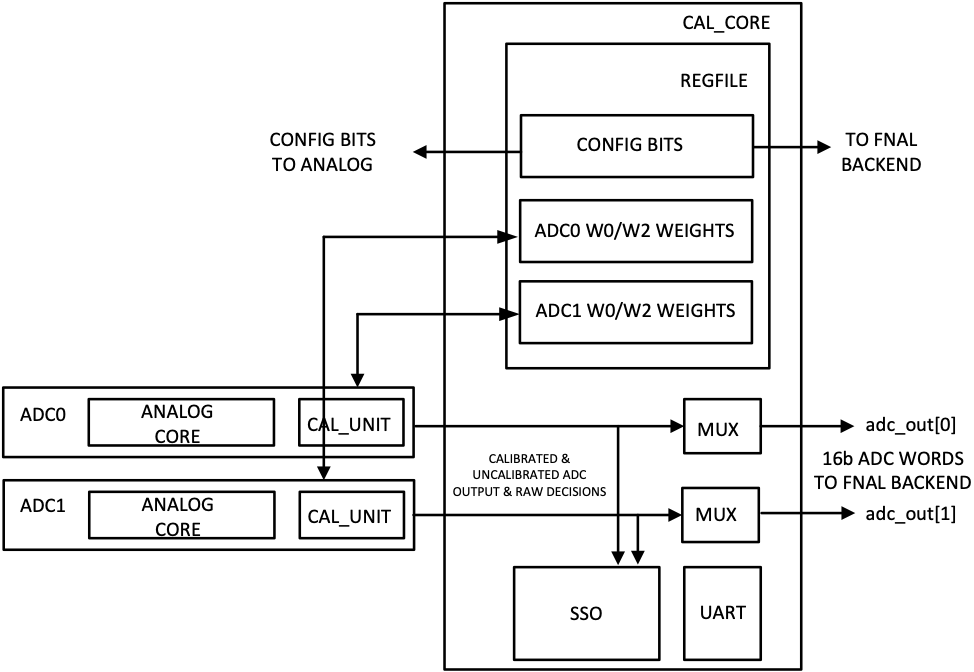
\includegraphics[width=1.0\textwidth]{figures/autocalBlock.png}
\end{center}
%\end{minipage}
\caption{Partitioning of Digital Logic in the ColdADC.}
\label{fig:autocalBlock}
\end{figure}


This would have been an acceptable strategy but due to miscommunication the interface between the cores was not simulated with back-annotated timing. This means that the timing when a computed calibration coefficient is written back into the registers was not simulated properly. When the blocks were placed, there was a timing error between the CAL\_UNIT and the CAL\_CORE in the case when the CAL\_UNIT was writing back computed calibration weights into storage in the CAL\_CORE.

An example of the intended operation is shown in Figure~\ref{fig:correctcalwrite}. In this simulation the CAL\_UNIT is back annotated with parasitics (but the interface with the CAL\_CORE is not properly back annotated). In this simulation, the intended data is in the second row (the word 0x03FD) and is written to the w2\_4 registerthat resides in the CAL\_CORE correctly. Correct operation is assured by disabling the memory after the edge of clk.
\begin{figure}[h]
\centering
%\begin{minipage}[b]{1.0\textwidth}
\begin{center}
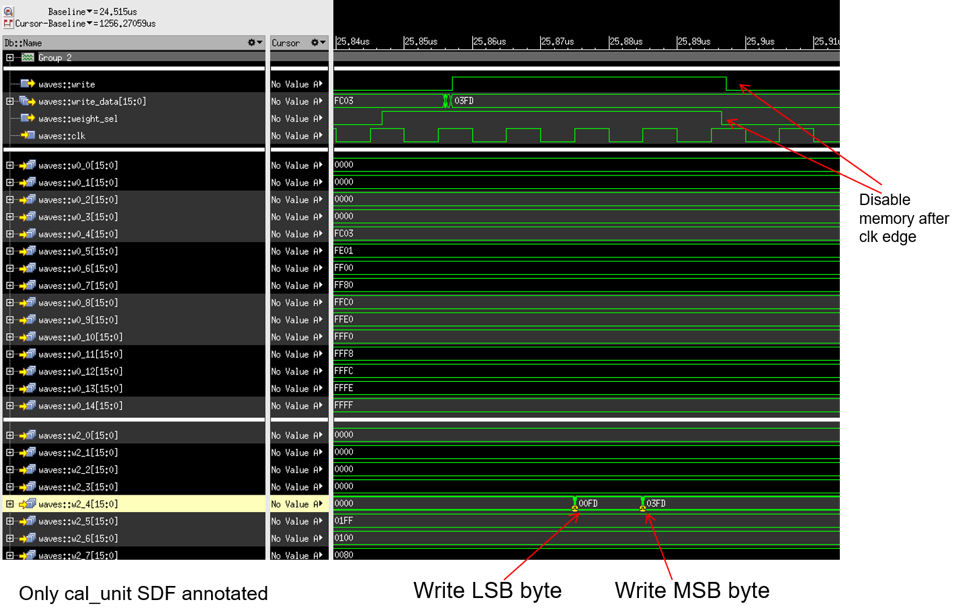
\includegraphics[width=1.0\textwidth]{figures/CorrectCalWrite.png}
\end{center}
%\end{minipage}
\caption{Correct writeback of calibration weights}
\label{fig:correctcalwrite}
\end{figure}

When the interface between CAL\_UNIT and CAL\_CORE was properly annotated and simulated, the result was in Figure~\ref{fig:errorcalwrite}.
\begin{figure}[htb]
\centering
%\begin{minipage}[b]{1.0\textwidth}
\begin{center}
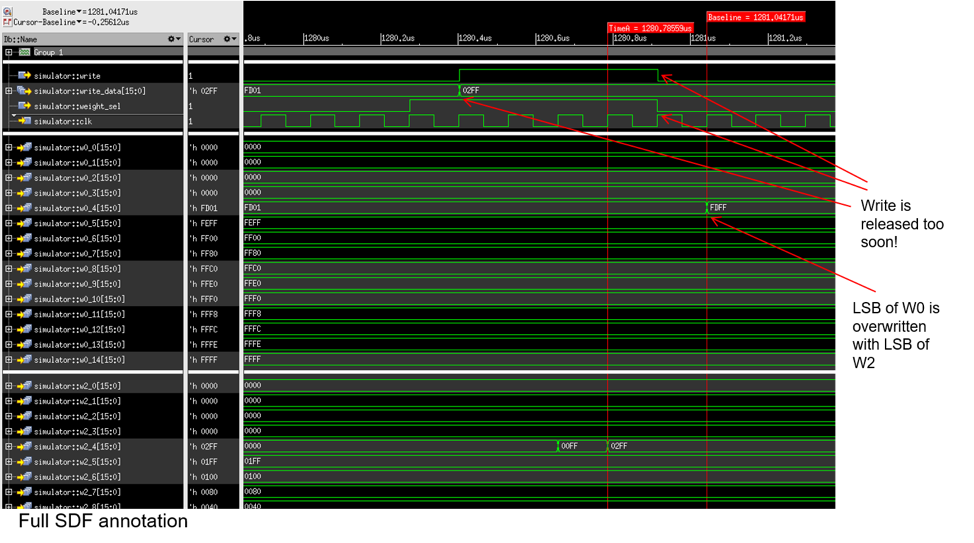
\includegraphics[width=1.0\textwidth]{figures/ErrorCalWrite.png}
\end{center}
%\end{minipage}
\caption{Error in writeback of calibration weights}
\label{fig:errorcalwrite}
\end{figure}
A gross error has been made, because the write signal is released too soon and therefore we have a race condition. What happens specifically here is that due to the race condition, the LSB byte of w0[4] is overwritten with the LSB byte of w2[4]. This is error and causes the entire calibration sequence to fail.

The fix here is to repartition the digital logic for the second version of the ColdADC ASIC. We will move the digital calibration and correction logic out of the ADCs and into a single, monolithic digital block. This will ensure that the interfaces between the calculation engines and the memory are simulated correctly and the absence of race conditions will be verified using static timing analysis. The RTL code itself will also be made more robust by adjusting the internal state machine.


\subsection{Level Shifter}
\label{sec:5.2}

%%%%%%%%%%%%%%%%%%%%%%%%%%%%%%%%%%%%%%%%%%%%%%%%%%%
% Level Shifter
%%%%%%%%%%%%%%%%%%%%%%%%%%%%%%%%%%%%%%%%%%%%%%%%%%%

Because the digital core of the Cold ADC uses 1.2 V rails, but many of the analog circuits on the chip use 2.5 V rails, level shifters are required to translate control settings from the 1.2 V voltage domain to the 2.5 V voltage domain. Unfortunately, due to confusion during the design process, the required level shifters that were required for the front end single-ended-to-differential input buffer were not included. Therefore, in order to configure the block correctly, the 1.2 V digital supply must be elevated. While this allows the chip to be operated successfully, it is not compatible with long-term reliability. The fix is to include the proper level shifters in the next version of Cold ADC. The fix has already been made in the layout.


\clearpage
\newpage
\subsection{ADC Core Linearity }
\label{sec:5.3}
%\clearpage
%%%%%%%%%%%%%%%%%%%%%%%%%%%%%%%%%%%%%%%%%%%%%%%%%%%%%%%
%(Prakash/Grace) Discuss ADC Core linearity
%%%%%%%%%%%%%%%%%%%%%%%%%%%%%%%%%%%%%%%%%%%%%%%%%%%%%%%
The measured ADC INL of the Cold ADC is approximately 1 LSB at a 12-bit level. However, simulations suggest 0.5 LSB INL after calibration is possible. The key reasons for the discrepancy is the lack of corner models at cold and the Monte Carlo analysis done using the warm models was insufficient. Testing indicates the ADC linearity is limited primarily by insufficient op-amp gain in the stages. Since the calibration algorithm can only correct linear gain error, higher-order non-linearity beyond what was expected limited the performance. The op-amp becomes nonlinear as their swing increases because the output resistance of the devices connected to the output decreases when the voltage across them is reduced. This is a known issue and was mitigated in the design by increasing the open-loop gain. The main suspect in the reduced linearity is that the raw open-loop gain is lower than expected and therefore the closed-loop rejection of the non-linearity is not good enough. To verify the large closed-loop gain non-linearity in the stages, we adjusted the reference voltages to reduce the dynamic range of each stage and this improved the linearity, as it should if the nonlinearity steps from the output stages of the op-amps. This is demonstrated in Figure~\ref{fig:linearity_100mv} and~\ref{fig:linearity_200mv}. In Figure~\ref{fig:linearity_100mv}, the differential reference is reduce 100 mV from nominal, and in Figure~\ref{fig:linearity_200mv} the differential reference is reduced 200 mV from nominal. Comparing Figures~\ref{fig:linearity_100mv} and \ref{fig:linearity_200mv}, the DNL is improved and becomes more uniform as the reference is reduced. 

\begin{figure}[h!]
\centering
  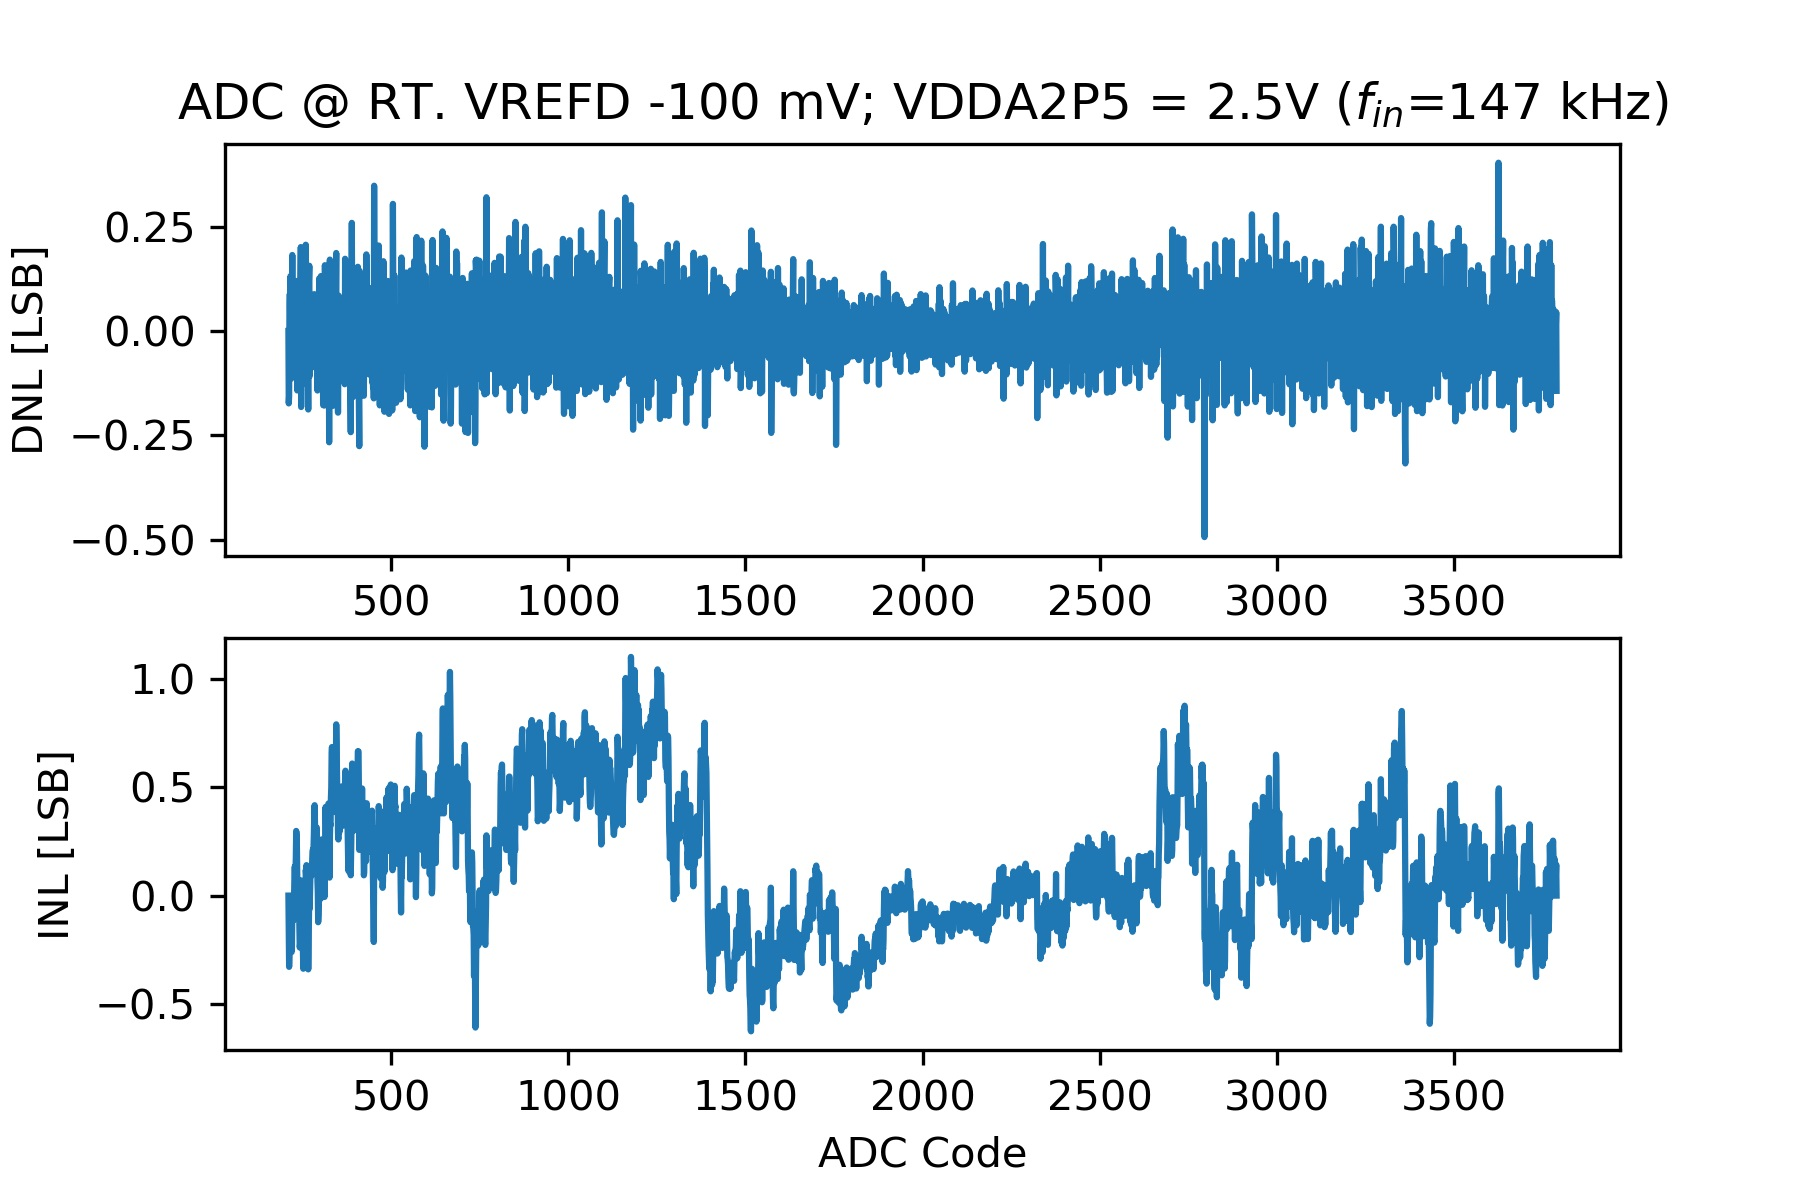
\includegraphics[width=0.7\linewidth]{figures/prakash_fig/linearity_100mv.JPG}
  \caption{ADC linearity with VREFN/P +/- 100mV}
  \label{fig:linearity_100mv}
\end{figure}

\begin{figure}[h!]
\centering
  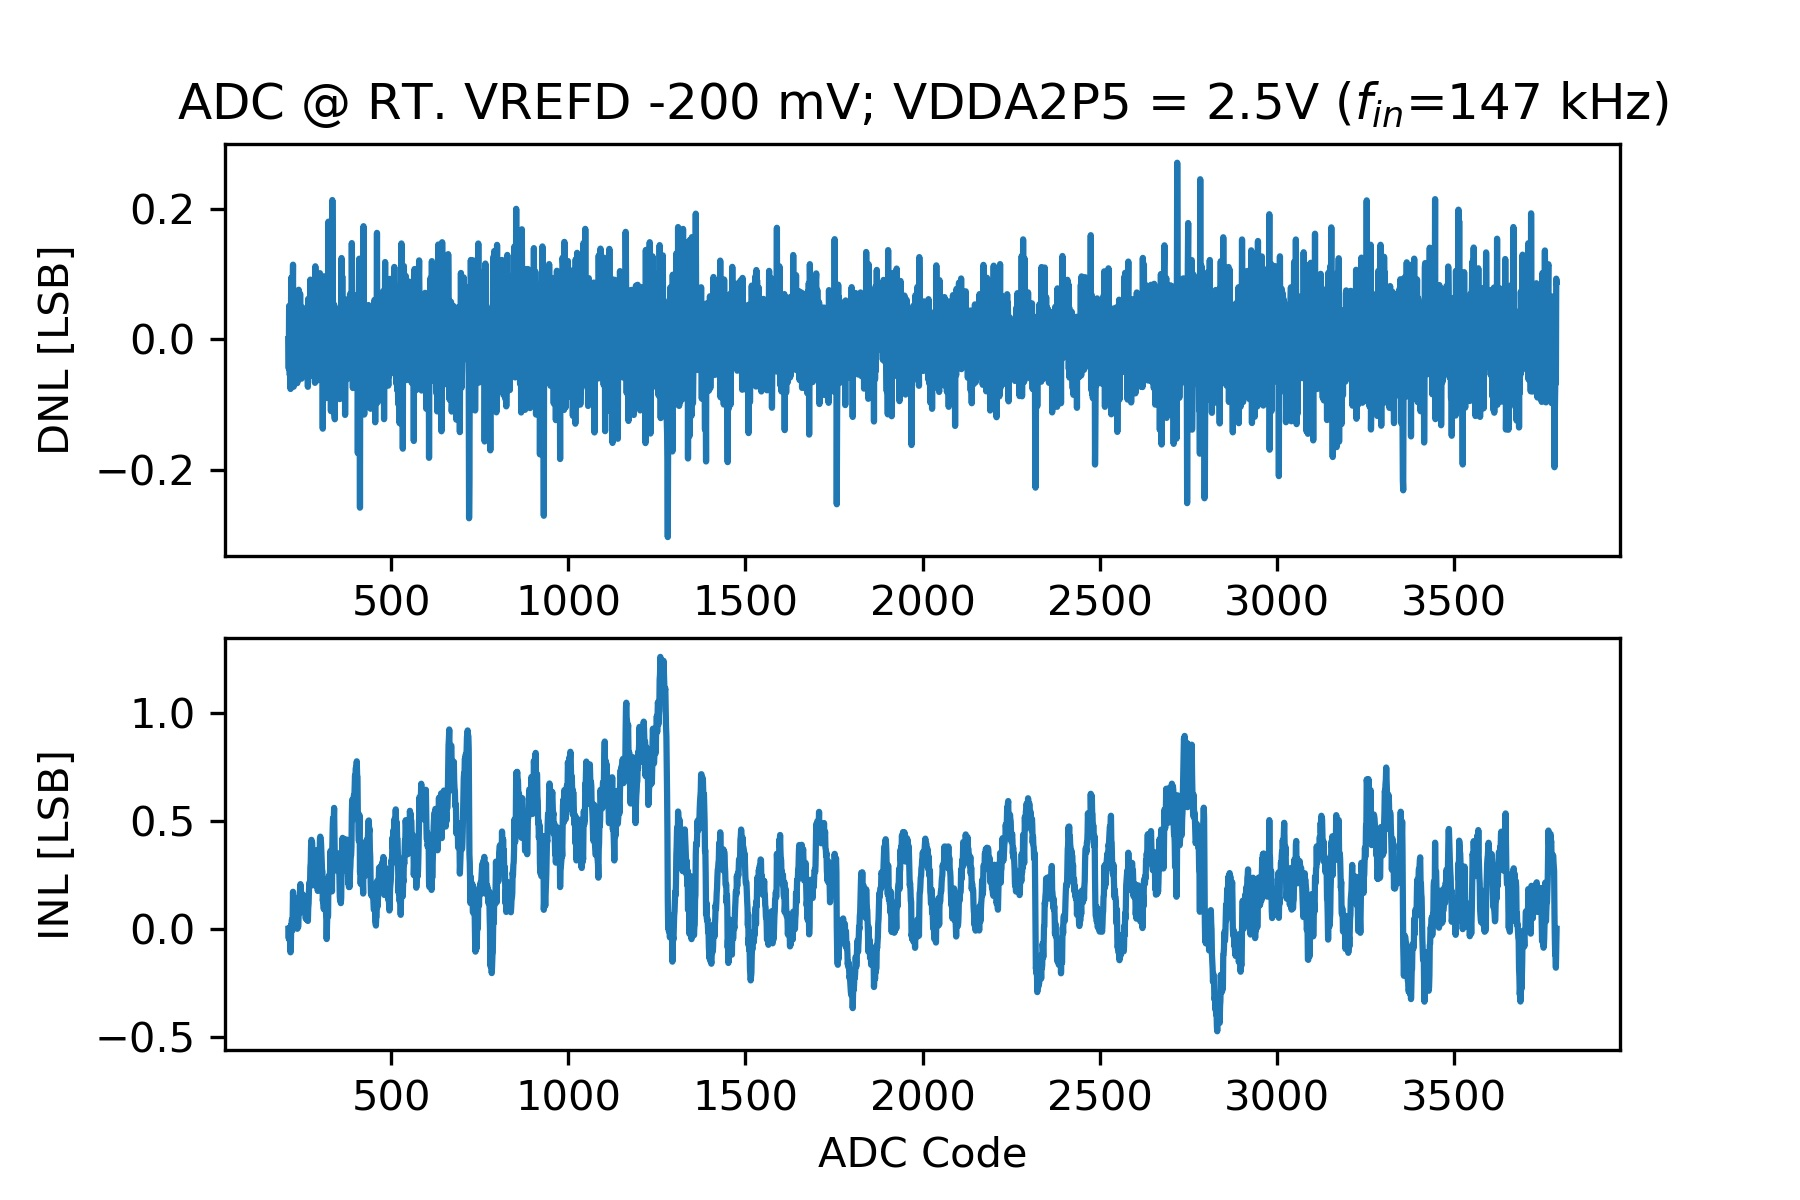
\includegraphics[width=0.7\linewidth]{figures/prakash_fig/linearity_200mv.JPG}
  \caption{ADC linearity with VREFN/P +/- 200mV}
  \label{fig:linearity_200mv}
\end{figure}

%\begin{figure}[h!]
%\centering
%  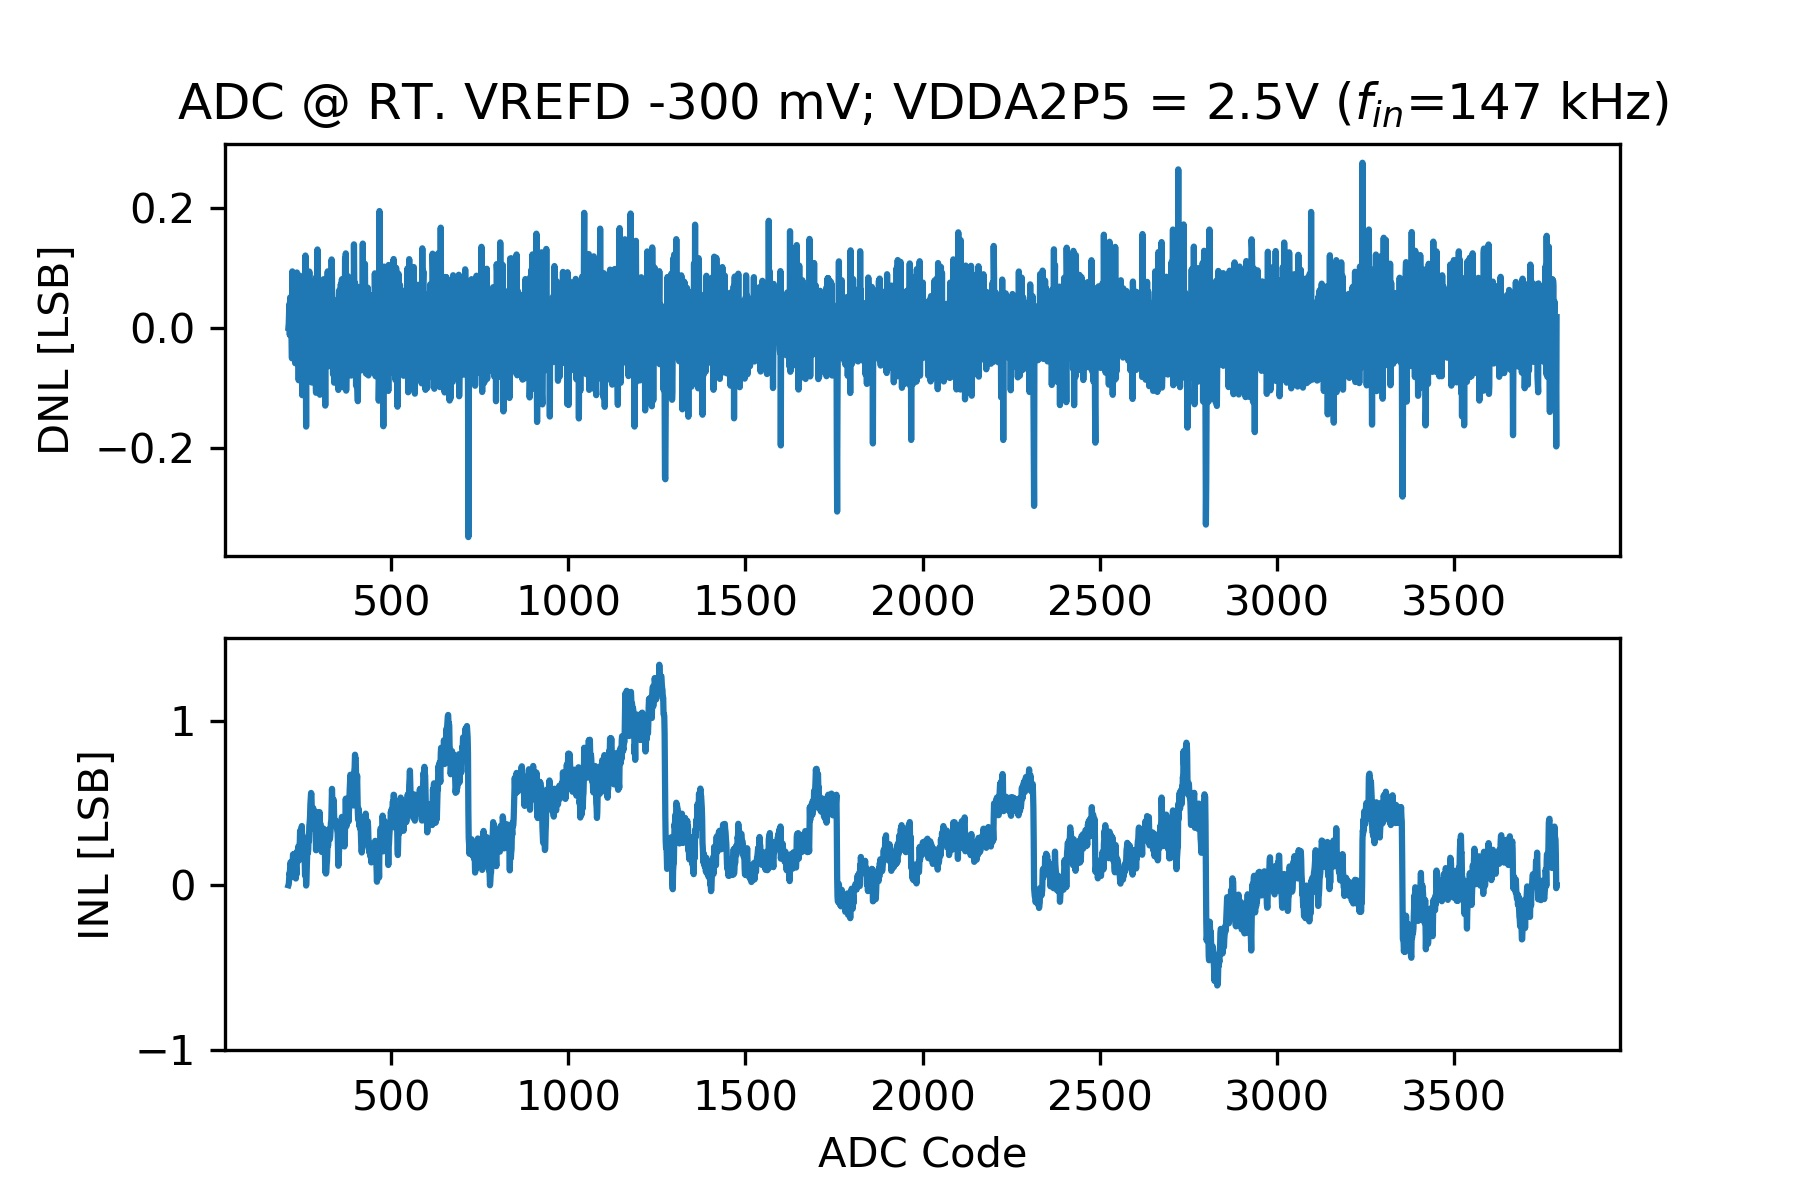
\includegraphics[width=0.7\linewidth]{figures/prakash_fig/linearity_300mv.JPG}
%  \caption{ADC linearity with VREFN/P +/- 300mV}
%  \label{fig:linearity_300mv}
%\end{figure}

To get evidence about what is the root cause of the increased linearity, we can use the programmability of the ColdADC to run various experiments to rule out potential causes. To rule out that the observed nonlinearity was caused by incomplete stage settling, we first operated the ADC with increased bias currents, to reduce settling time. This did not improve performance. We then slowed down the ADC by a factor of 16 and reduced the op-amp bias currents. Reducing the bias currents has the effect of increasing the op-loop gain, but also slows down the circuit, necessitating the reduced sampling rate. 
The results of this experiment is shown in Figure~\ref{fig:linearity_GB_ON}. The ColdADC demonstrates superior performance in this situation, strongly suggesting the increased open-loop gain mitigates the gain-drooping caused by the op-amp output resistance. Note that the references are nominal here, showing that the observed nonlinearity it reduced in this case by the negative feedback.

\begin{figure}[h!]
\centering
  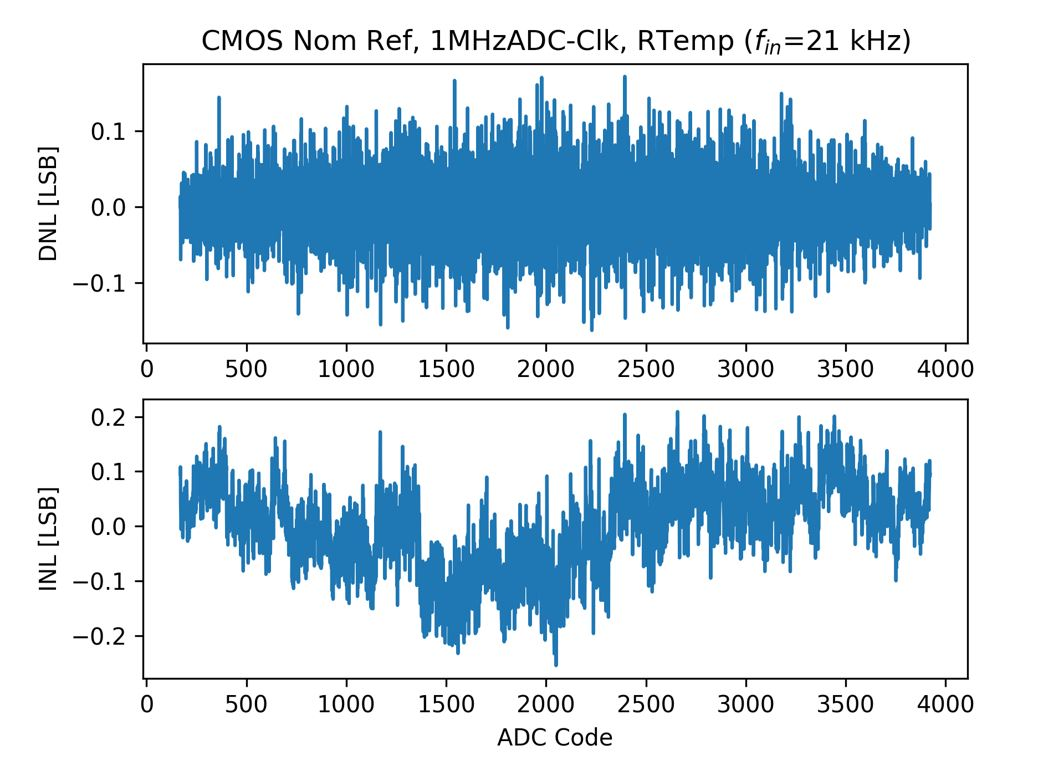
\includegraphics[width=0.7\linewidth]{figures/prakash_fig/linearity_GB_ON.JPG}
  \caption{Linearity with Gain Boosters ON}
  \label{fig:linearity_GB_ON}
\end{figure}

A schematic of the op-amp used in the ADC stages is shown in Figure~\ref{fig:op_amp_1}. The circuit uses a standard folded-cascode topology with gain boosting amplifiers used to increase the open-loop gain. These gain boosting amplifiers work by regulating the voltage drop across the output transistors, increasing their output resistance. Simulations suggested that the gain boosting amplifiers increased the open-loop gain of the op-amp by approximately a factor of 5 (14 dB).

\begin{figure}[h!]
\centering
  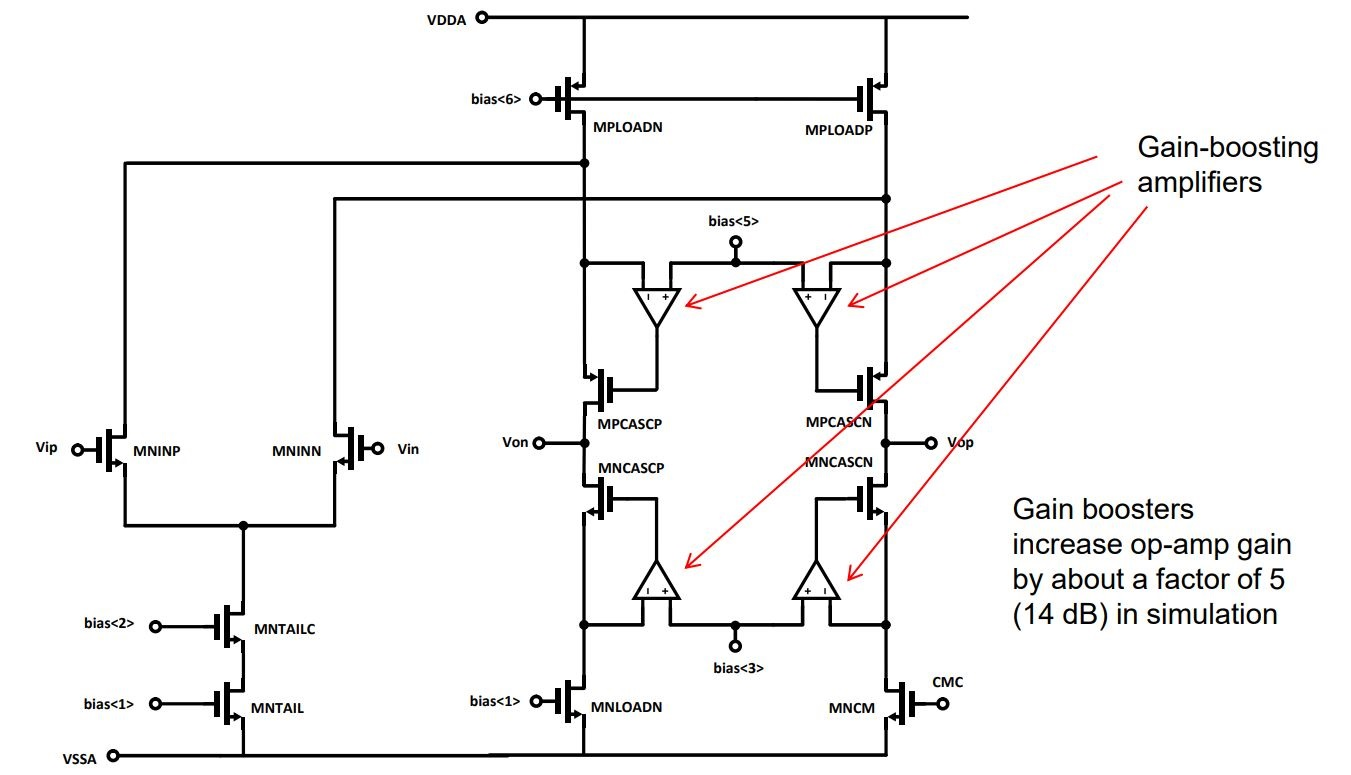
\includegraphics[width=0.9\linewidth]{figures/prakash_fig/op_amp.JPG}
  \caption{Op-Amp used in ColdADC stages.}
  \label{fig:op_amp_1}
\end{figure}

To narrow down what precisely in the op-amp was causing the lower-than-expected gain, we disabled the gain boosting amplifiers. This is possible to do through the configuration interface and was included for debugging purposes. When we disabled the gain boosting amplifiers, but held all other conditions constant, the linearity degraded as shown in Figure~\ref{fig:linearity_GB_OFF}. In fact, the INL increased by over a factor of 2 and the DNL increased as well.


\begin{figure}[h!]
\centering
  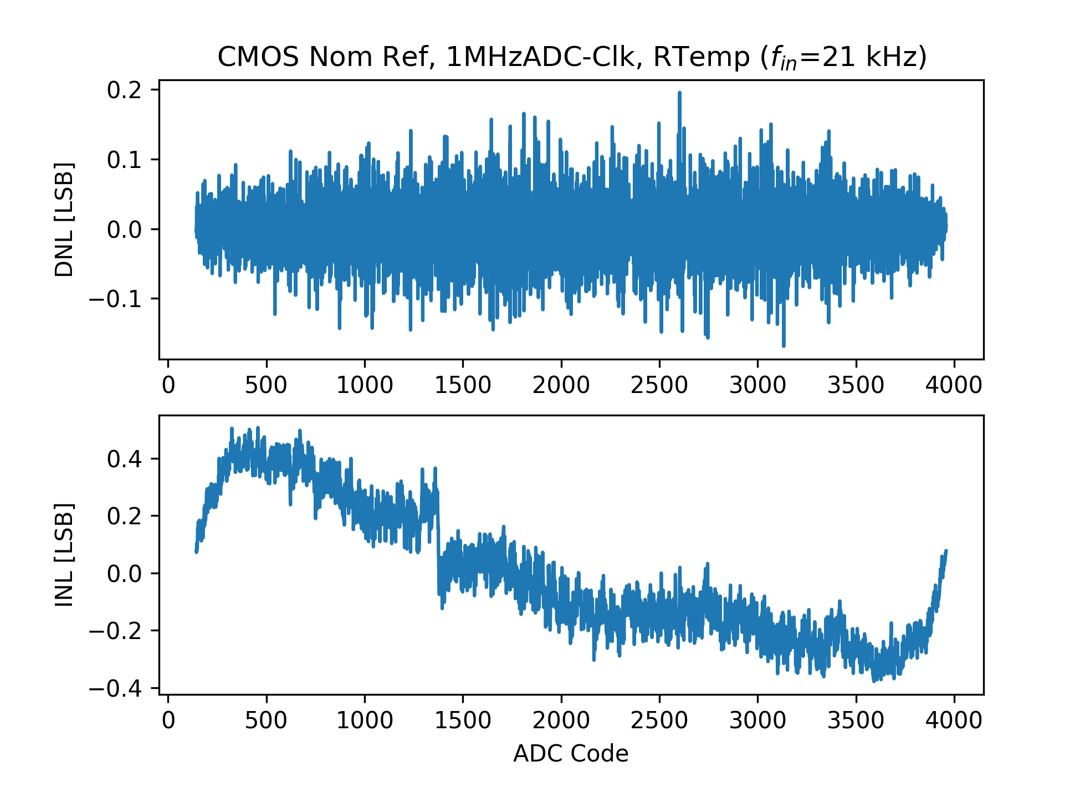
\includegraphics[width=0.7\linewidth]{figures/prakash_fig/linearity_GB_OFF.JPG}
  \caption{Linearity with Gain Boosters OFF.}
  \label{fig:linearity_GB_OFF}
\end{figure}

For further evidence, we modeled the ADC behaviorally using MATLAB. The simulated linearity obtained after setting the op-amp open-loop gain in the model to 80 dB is shown in Figure~\ref{fig:behav_GB_ON}, which is a result similar to Figure~\ref{fig:linearity_GB_ON}. By reducing the open-loop gain to 74 dB, we obtained the result in Figure~\ref{fig:behav_GB_OFF} which closely follows the linearity structure of Figure~\ref{fig:linearity_GB_OFF}. This gives further evidence the issue is insufficient gain in the gain boosting amplifiers. Based on the behavioral modeling, we estimate the gain-boosting amplifiers are providing approximately 6 dB in additional gain, rather than the 14 dB that was expected.
\begin{figure}[h!]
\centering
  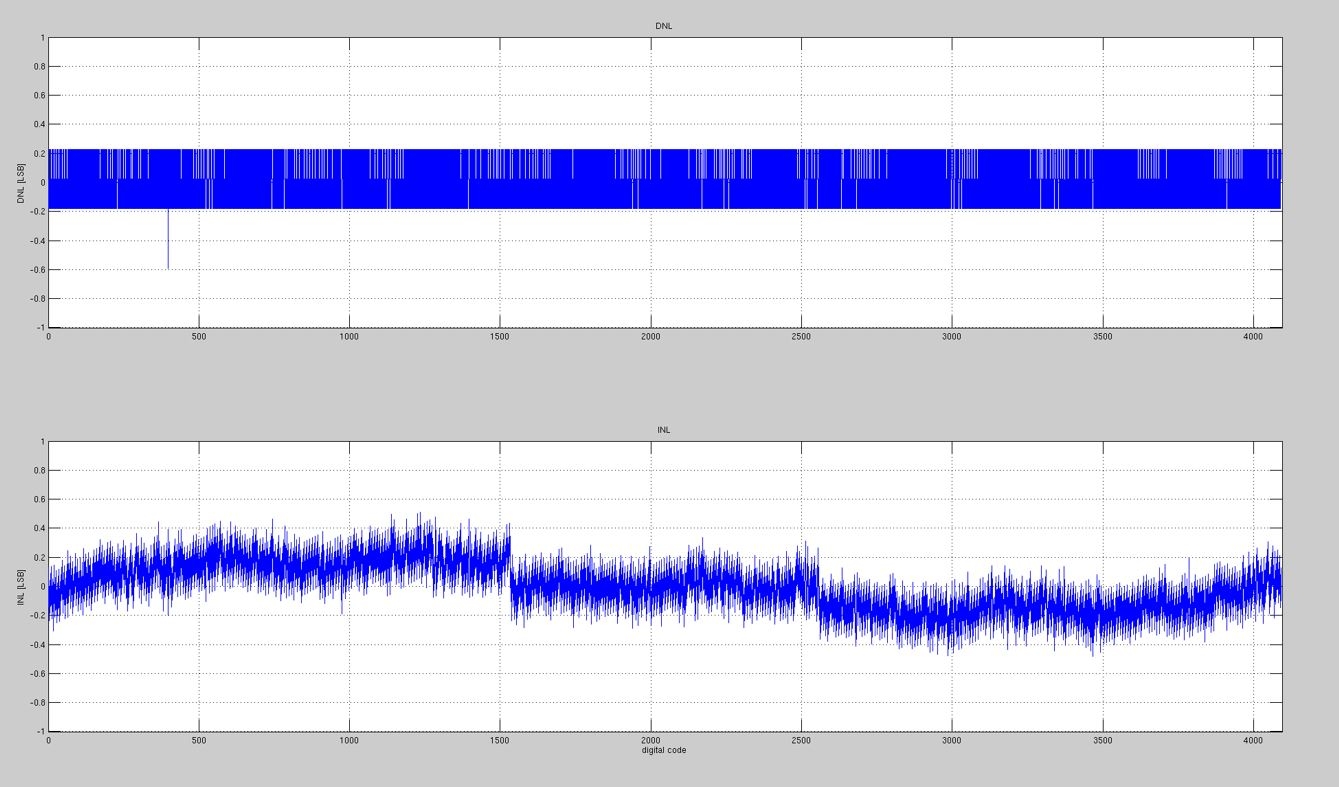
\includegraphics[width=0.7\linewidth]{figures/prakash_fig/behav_GB_ON.JPG}
  \caption{MATLAB model - gain boosters on -> 80 dB op-amp gain.}
  \label{fig:behav_GB_ON}
\end{figure}

\begin{figure}[h!]
\centering
  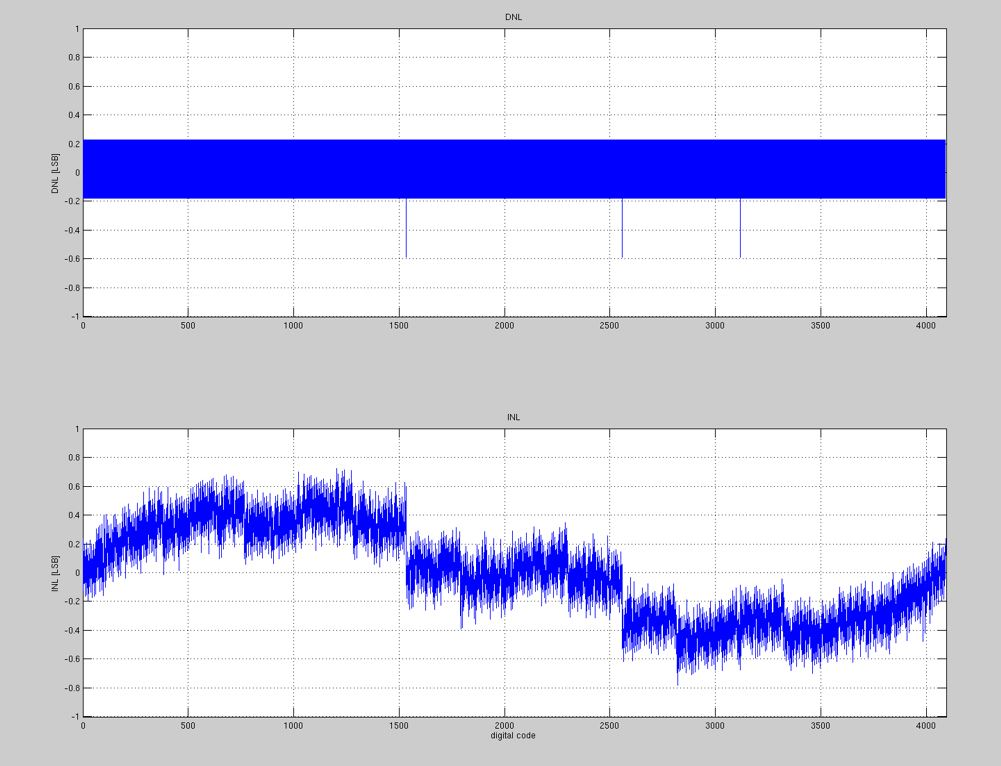
\includegraphics[width=0.7\linewidth]{figures/prakash_fig/behav_GB_OFF.JPG}
  \caption{MATLAB model - gain boosters off -> 74 dB op-amp gain.}
  \label{fig:behav_GB_OFF}
\end{figure}
Analysis of the circuits in the gain-boosting amplifiers indicates that they may have insufficient design margin in their biasing networks. The gain-boosting amplifiers and op-amp can be improved by redesigning them to better center their operating points across process and temperature.

Corner analysis of the complete op-amp before and after the gain-boosting redesign is shown in Figures~\ref{fig:opamp_gain_rt} and \ref{fig:opamp_gain_m_rt}, respectively. While the corners are only strictly valid at room temperature, the take away here is that the minimum open-loop gain across corners after the redesign is higher than the maximum open-loop gain before redesign. The design fix is being finalized and will soon be implemented in the layout.

\begin{figure}[h!]
\centering
  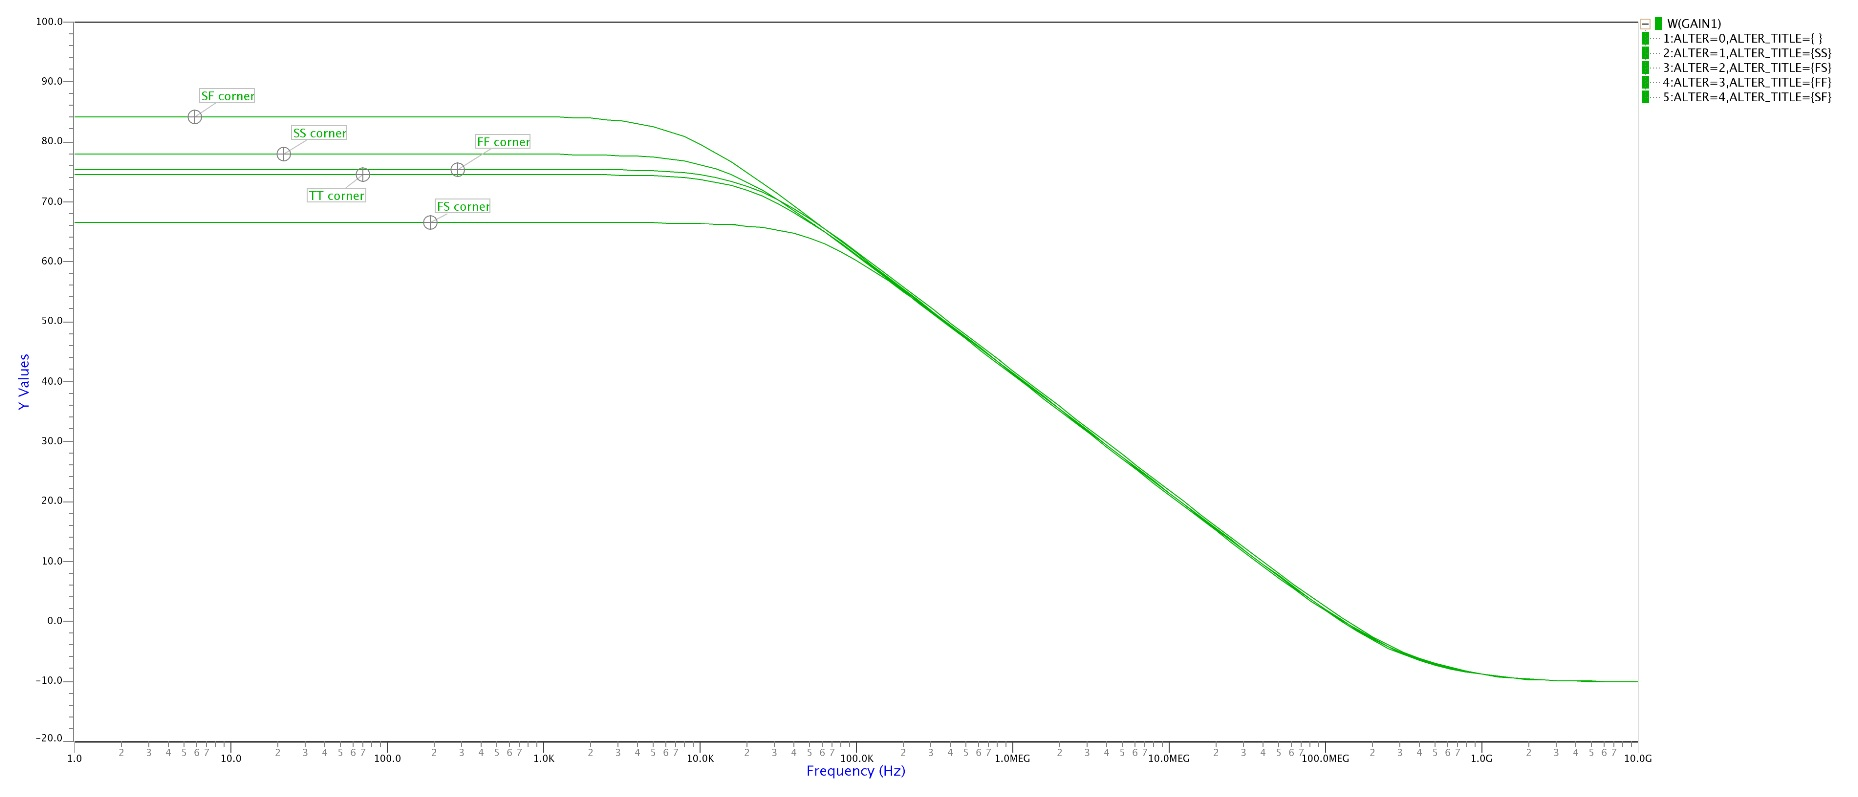
\includegraphics[width=0.8\linewidth]{figures/prakash_fig/opamp_gain_rt.JPG}
  \caption{Corner analysis of the op-amp gain, with current gain booster circuit.}
  \label{fig:opamp_gain_rt}
\end{figure}

\begin{figure}[h!]
\centering
  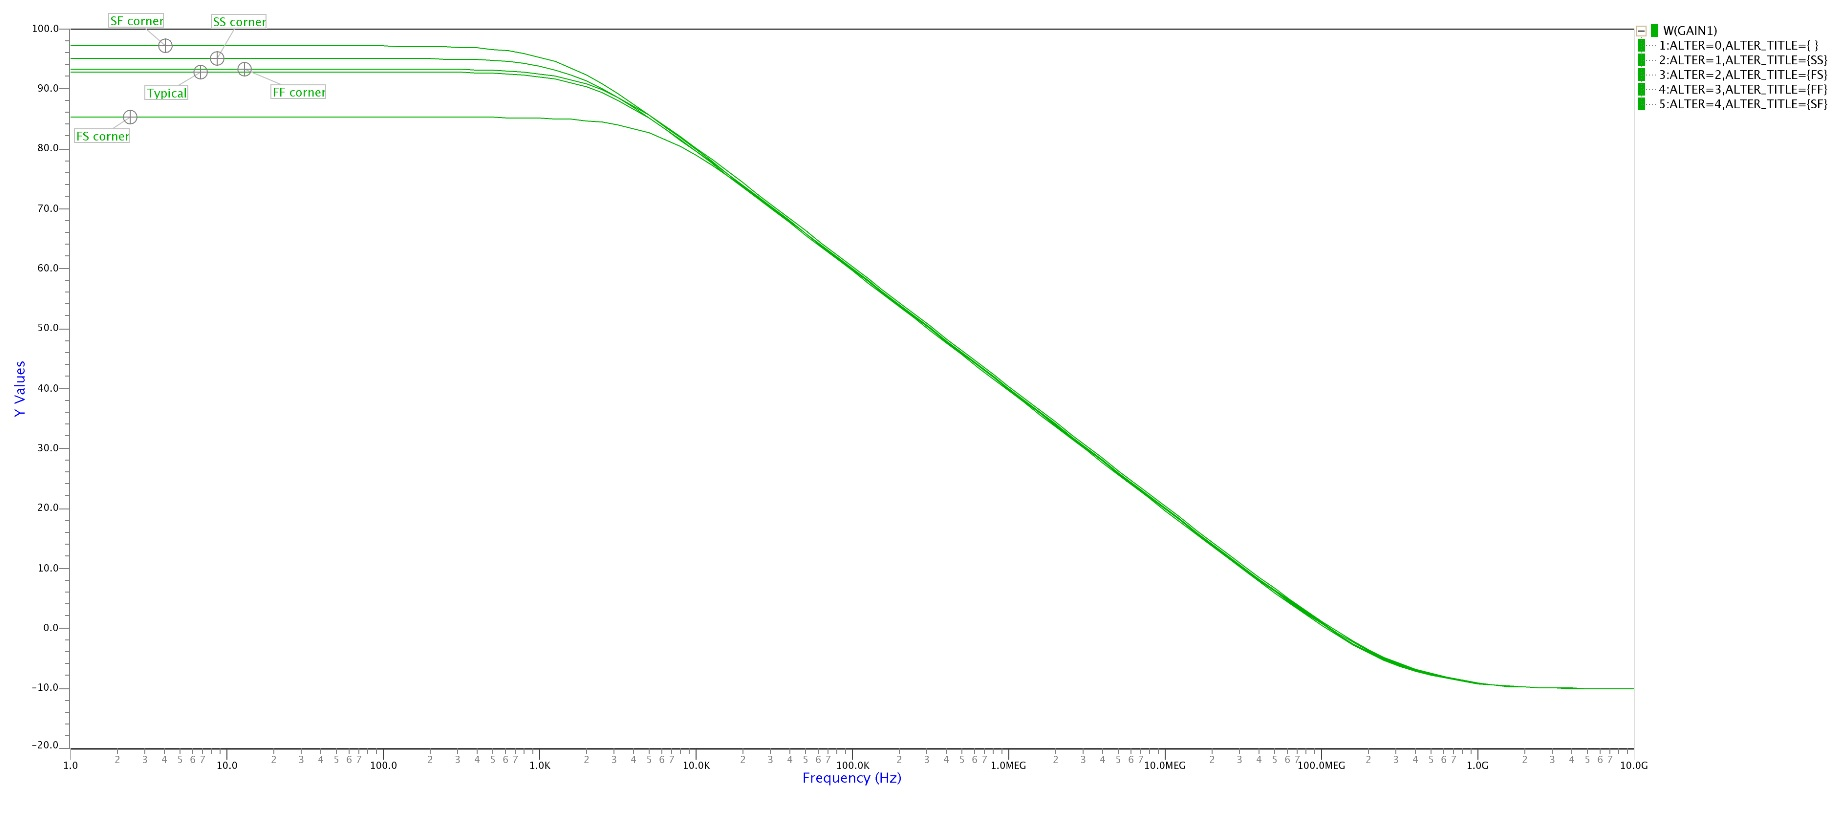
\includegraphics[width=0.8\linewidth]{figures/prakash_fig/opamp_gain_m_rt.JPG}
  \caption{Corner analysis of the op-amp gain, with improved gain booster circuit.}
  \label{fig:opamp_gain_m_rt}
\end{figure}


\clearpage
\newpage
\subsection{SHA/MUX Linearity  }
\label{sec:5.4}

%%%%%%%%%%%%%%%%%%%%%%%%%%%%%%%%%%%%%%%%%%%%%%%%%%%%%%%
%(Prakash) Discuss SHA/MUX linearity
%%%%%%%%%%%%%%%%%%%%%%%%%%%%%%%%%%%%%%%%%%%%%%%%%%%%%%%

The input signals are sampled at a rate of 2 MS/s, multiplexed by 8 and digitized by one of two calibrated 12-bit pipelined ADCs operating at 16 MS/s. The linearity of the ADC to a small extent depends on the linearity of the SHA/MUX circuit aswell. 

ColdADC can be calibrated to an amazing degree. The ability to configure and isolate the MUX's turned out to be very helpful to debug the SHA/MUX linearity issue. The linearity of the ADC is approximately reduced by 0.3 LSB when SHA is in free running mode (MUX is operating). 

%Studies were performed at two configuration settings, forzen SHA mode and free running SHA mode. Nominal operation is free running SHA mode. 

During the Frozen SHA mode, the ADC will oversample the SHA output by a factor of 8 and the linearity of the ADC can be calculated by taking any of the samples. We observed that the overall linearity was different for different sample sets. Figure \ref{fig:sha_sample_hist} shows ADC sampling with frozen SHA.

\begin{figure}[h!]
\centering
  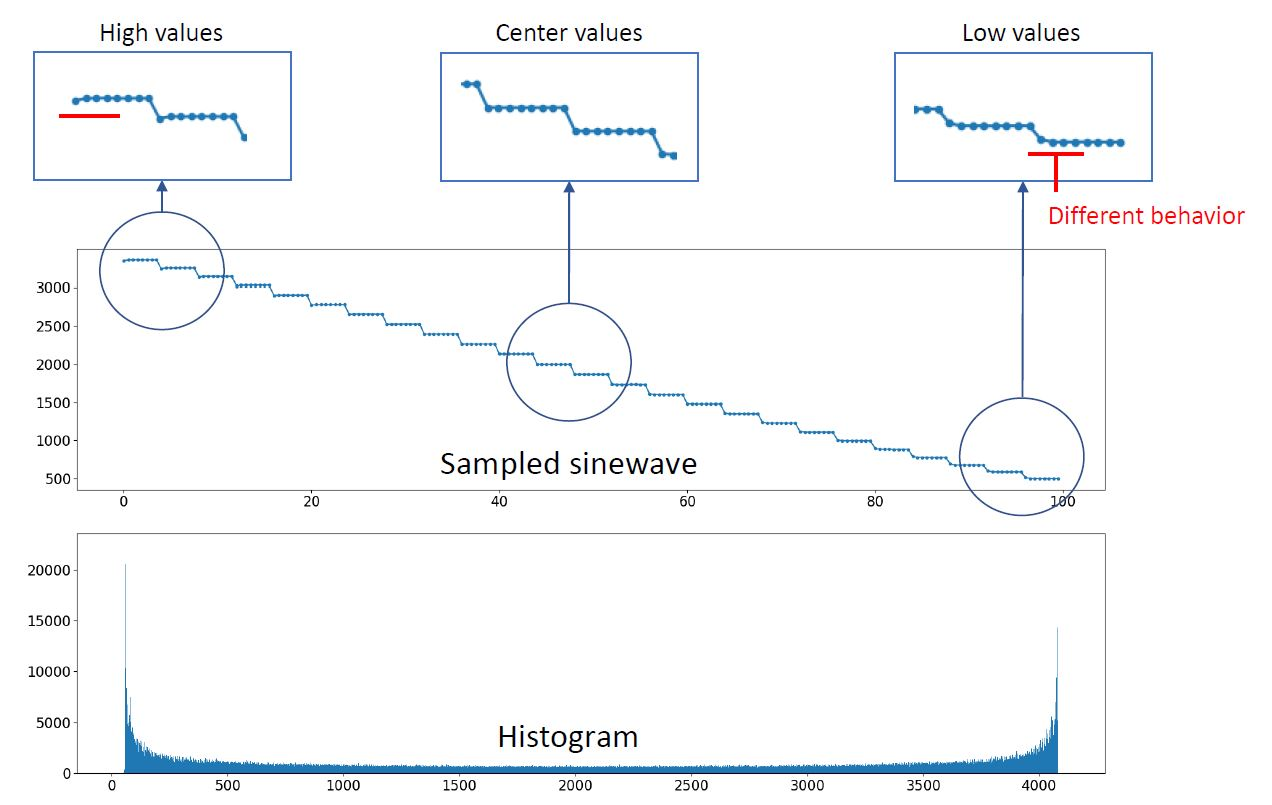
\includegraphics[width=0.7\linewidth]{figures/prakash_fig/sha_sample_hist.JPG}
  \caption{Histogram of ADC sampling in frozen SHA configuration}
  \label{fig:sha_sample_hist}
\end{figure}

The non-linearity could be affected by SHA or MUX or a combination of both. To verify if the SHA op-amps are causing any non-linearity. Figures \ref{fig:linearity_sha_40u}, \ref{fig:linearity_sha_50u} and \ref{fig:linearity_sha_60u} show the linearity of ADC measured by looking at the second sample of channel 7 at 40$\mu$A, 50$\mu$A (default) and 60$\mu$A bias currents. 

\begin{figure}[h!]
\centering
  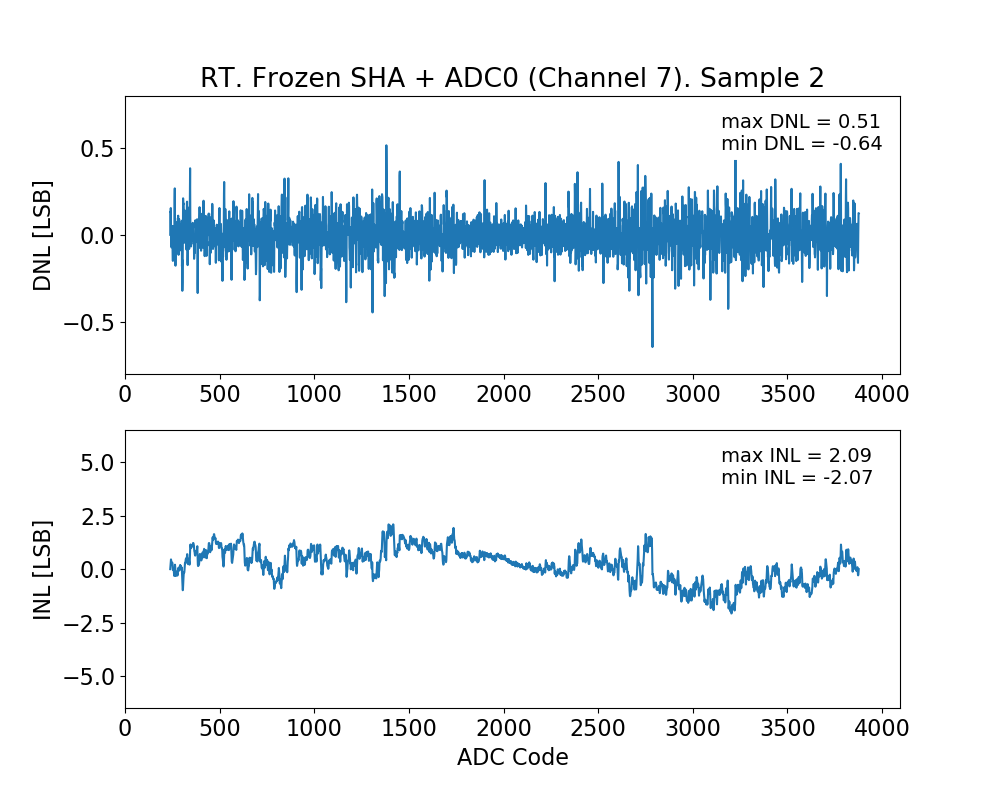
\includegraphics[width=0.7\linewidth]{figures/prakash_fig/linearity_sha_40u.png}
  \caption{Linearity of ADC at room temperature with SHA bias current configured to 40$\mu$A}
  \label{fig:linearity_sha_40u}
\end{figure}
\begin{figure}[h!]
\centering
  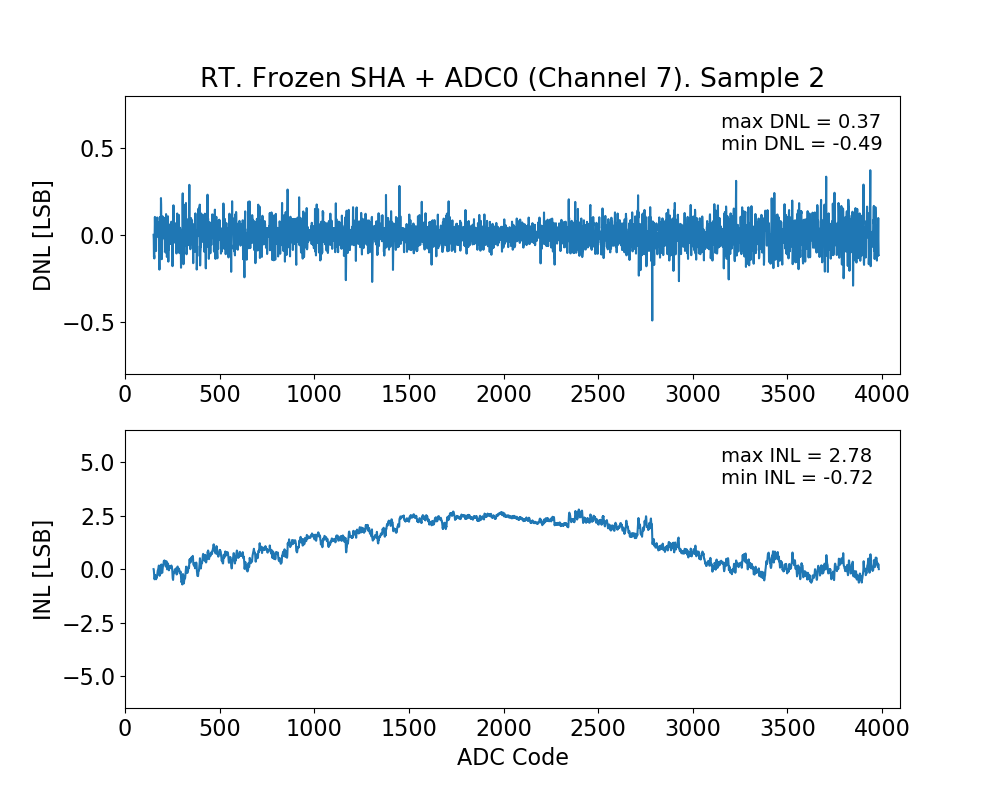
\includegraphics[width=0.7\linewidth]{figures/prakash_fig/linearity_sha_50u.png}
  \caption{Linearity of ADC at room temperature with SHA bias current configured to 50$\mu$A, this the nominal SHA bias current}
  \label{fig:linearity_sha_50u}
\end{figure}
\begin{figure}[h!]
\centering
  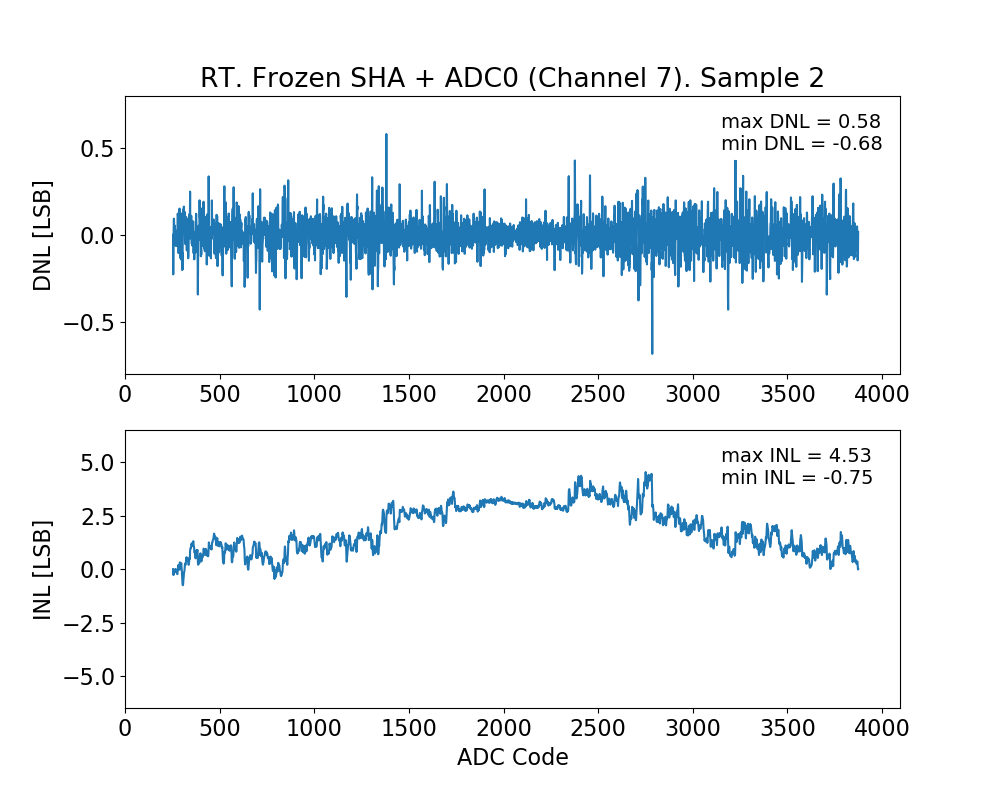
\includegraphics[width=0.7\linewidth]{figures/prakash_fig/linearity_sha_60u.png}
  \caption{Linearity of ADC at room temperature with SHA bias current configured to 60$\mu$A}
  \label{fig:linearity_sha_60u}
\end{figure}

Varying the SHA bias currents did not affect the overall linearity of the ADC. To verify if the MUX's were causing the non-linearity, we reduced the sampling speed. Figures \ref{fig:linearity_mux_2M}, \ref{fig:linearity_mux_1M} and \ref{fig:linearity_mux_500K} show the linearity at different sampling clocks. 
\begin{figure}[h!]
\centering
  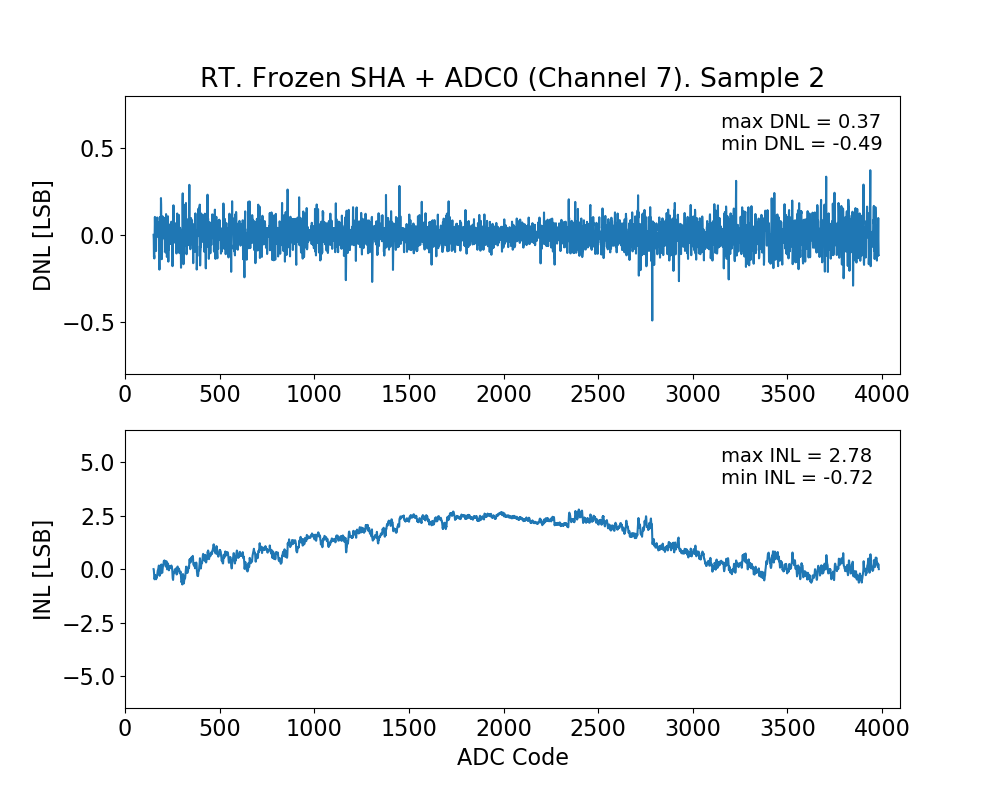
\includegraphics[width=0.7\linewidth]{figures/prakash_fig/linearity_mux_2M.png}
  \caption{Linearity of ADC at room temperature with 2MHz sampling frequency (16MS/s ADC)}
  \label{fig:linearity_mux_2M}
\end{figure}

\begin{figure}[h!]
\centering
  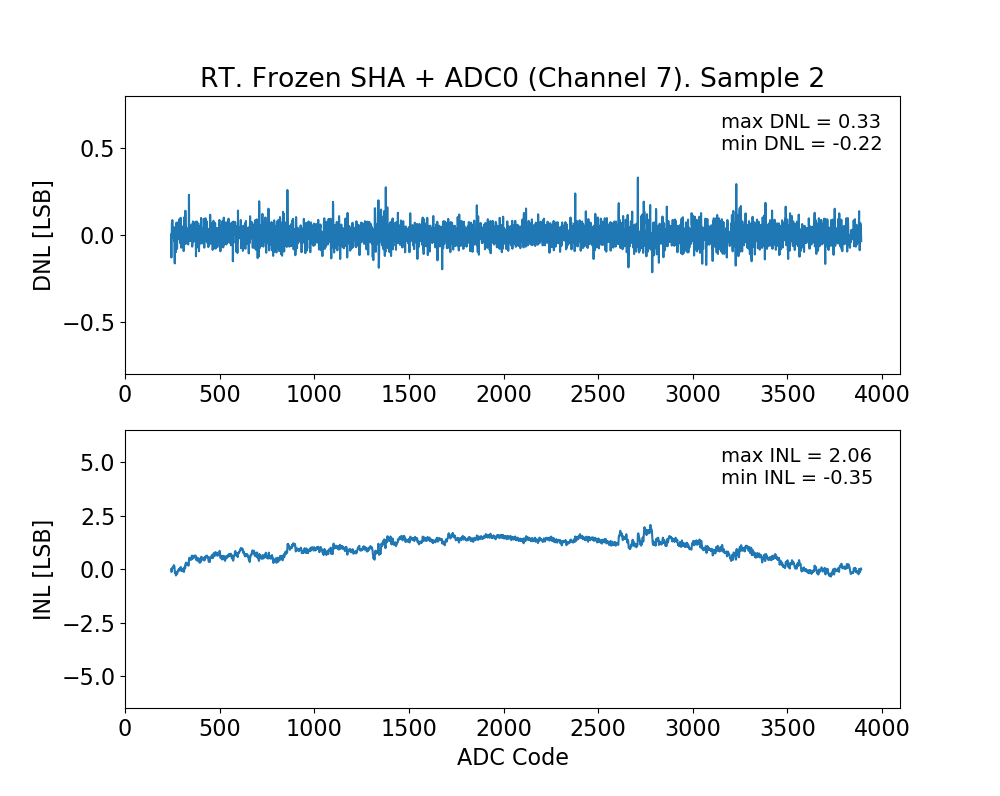
\includegraphics[width=0.7\linewidth]{figures/prakash_fig/linearity_mux_1M.png}
  \caption{Linearity of ADC at room temperature with 1MHz sampling frequency (8MS/s ADC)}
  \label{fig:linearity_mux_1M}
\end{figure}

\begin{figure}[h!]
\centering
  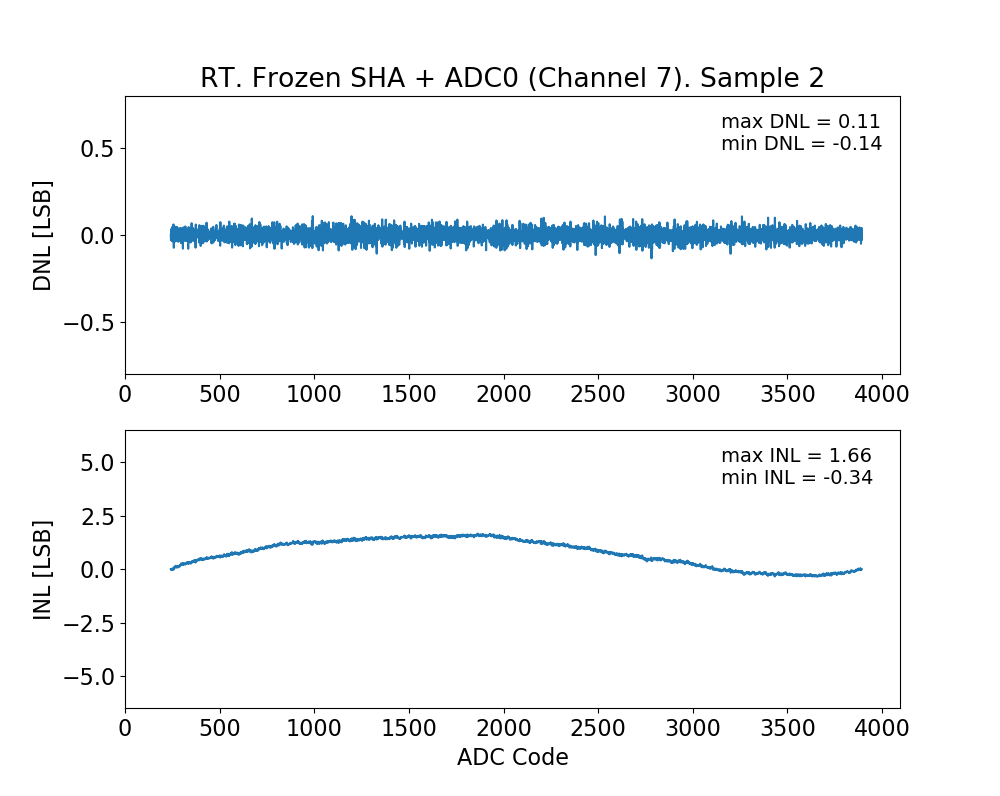
\includegraphics[width=0.7\linewidth]{figures/prakash_fig/linearity_mux_500K.png}
  \caption{Linearity of ADC at room temperature with 500kHz sampling frequency (4MS/s ADC)}
  \label{fig:linearity_mux_500K}
\end{figure}

Reducing the sampling frequency improves the linearity significantly. The MUX's seem to be causing the non-linearity and we believe the kickback is the main source of the problem. To fix this problem we have to redesign the MUX to be much faster. 

We also observed spikes in the DNL plots while the ColdADC was configured to free running SHA mode. These spikes however reduced when he ColdADC was configured to frozen SHA mode. Figures \ref{fig:linearity_freesha} and \ref{fig:linearity_frozensha} show the difference in linearity for free running and frozen SHA. These measurements were performed with nominal clocks and nominal reference voltages.  

\begin{figure}[h!]
\centering
  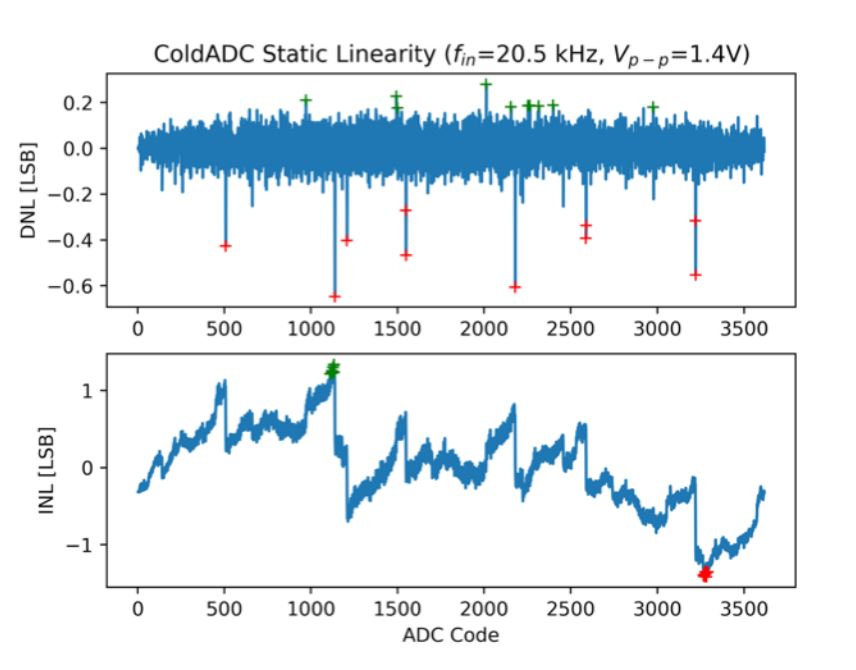
\includegraphics[width=0.7\linewidth]{figures/prakash_fig/linearity_freesha.JPG}
  \caption[Linearity of the ADC with single ended input with free running SHA]{Linearity of the ADC with single ended input with free running SHA: These measurements were taken at LN2 temperature. During the free running SHA configuration, the MUX's introduces additional spikes in the DNL}
  \label{fig:linearity_freesha}
\end{figure}

\begin{figure}[h!]
\centering
  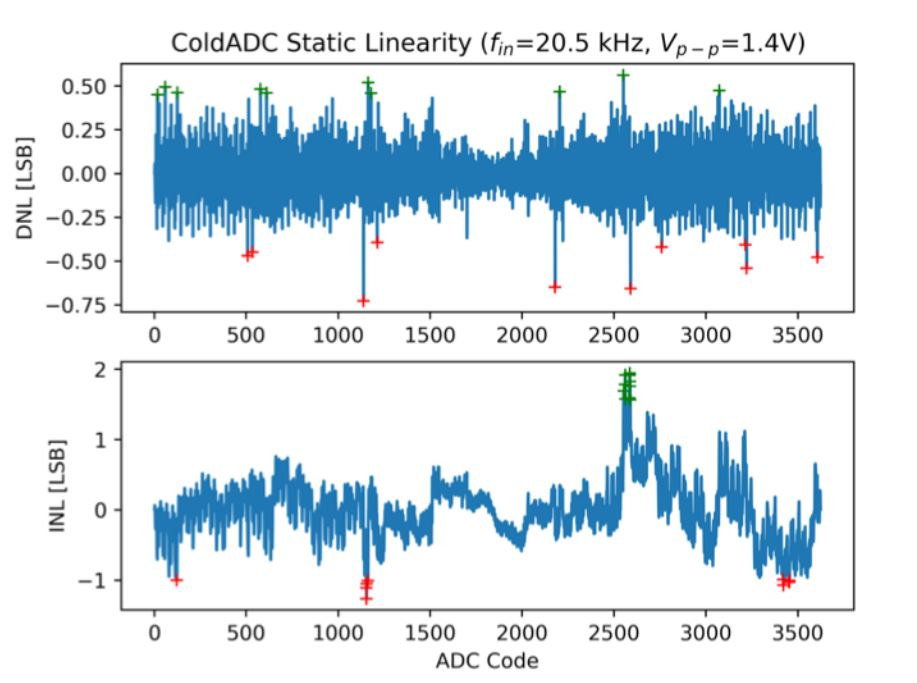
\includegraphics[width=0.7\linewidth]{figures/prakash_fig/linearity_frozensha.JPG}
  \caption[Linearity of the ADC with single ended input with frozen SHA]{Linearity of the ADC with single ended input with frozen SHA: These measurements were taken at LN2 temperature}
  \label{fig:linearity_frozensha}
\end{figure}

Another observation was that the DNL spikes were larger when the ASIC was cooled down, a possible explanation for this is the ON resistance of the switches (MUX) is significantly larger at cold than in warm. Redesigning the MUX to be faster will solve this problem aswell.  

Evidence of linearity degradation only during the free running SHA mode indicate couple other possible issues: possible overlapping of the clocks for the MUX's and/or insufficient settling of MUX's. It is very difficult to simulate MUX's effects on ADC linearity. We are still in the process of understanding and proving the root cause for linearity degradation in simulations. To fix this, we will redesign the MUX's to be faster and improve the clocking scheme. 



\clearpage
\newpage
\subsection{SDC Linearity }
\label{sec:5.5}

%%%%%%%%%%%%%%%%%%%%%%%%%%%%%%%%%%%%%%%%%%%%%%%%%%%
% (DABROWSKI) SDC Linearity
%%%%%%%%%%%%%%%%%%%%%%%%%%%%%%%%%%%%%%%%%%%%%%%%%%%

%A single ColdADC input channel comprises of an Input Buffer block followed by a Sample-and-Hold (SHA) circuit, followed by a multiplexer that multiplexes outputs of 8 channels to a single fully-differential ADC core. ColdADC contains two cores, therefore, channels from 0 to 7 are multiplexed to the first core and channels from 8 to 15 to the second one.

The ColdADC Input Buffer contains two blocks - a Single-to-Differential Converter (SDC) and a Differential Buffer (DB). The former one accepts single-ended signals and converts them to fully-differential ones, has a low-capacitance input-impedance, and drives the capacitive switching load of the SHA. The latter one buffers differential input signals, has a static capacitive input impedance, and drives the switching load of the SHA. Each of these two blocks can be separately powered-down and bypassed.

LArASIC outputs single-ended waveforms; therefore, the performance of each ADC input channel when accepting single-ended signals is of high importance. Single-ended input signals to the ADC can be converted to fully-differential signals in either a SDC or SHA block. The performance merit of primary interest are input channel DNL and INL at room (RT) and cryogenic temperatures (Liquid Nitrogen - LN) when driven by a single-ended source, with and without the SDC block.

Figures \ref{fig;sdc;inl_dnl_max_rt} and \ref{fig;sdc;inl_dnl_max_ln} show measurements of maximum INL and maximum DNL across all ADC channels at room and cryogenic temperatures, respectively. These were derived from measurements presented in Figures \ref{fig;sdc;dnl_all_rt}, \ref{fig;sdc;inl_all_rt}, \ref{fig;sdc;dnl_all_ln} and \ref{fig;sdc;inl_all_ln}. Figure \ref{fig;sdc;enob_rt} depicts ENOB across ADC channels with and without the SDC.

Measured results are insufficient in providing a conclusion as to whether the SDC block improves or deteriorates ADC's performance. However, measurements at LN temperature show slight improvment, on average, in DNL across channels with the SDC turned on. Measurements also indicate introduction of larger channel-to-channel variation in INL when the SDC is on. However, this might be related to bypass switches and/or other interfaces, not the SDC alone.

A standalone SDC circuit is currently being tested and a statistical analysis on a larger set of samples of standalone chips is also planned for. These results might help to answer some of the above questions/uncertainities.

Current recommendation is to remove the SDC block from the ADC input chain and implement it in the LArASIC channel.

\begin{figure}[ht!]
\begin{minipage}{.5\textwidth}
  \centering
  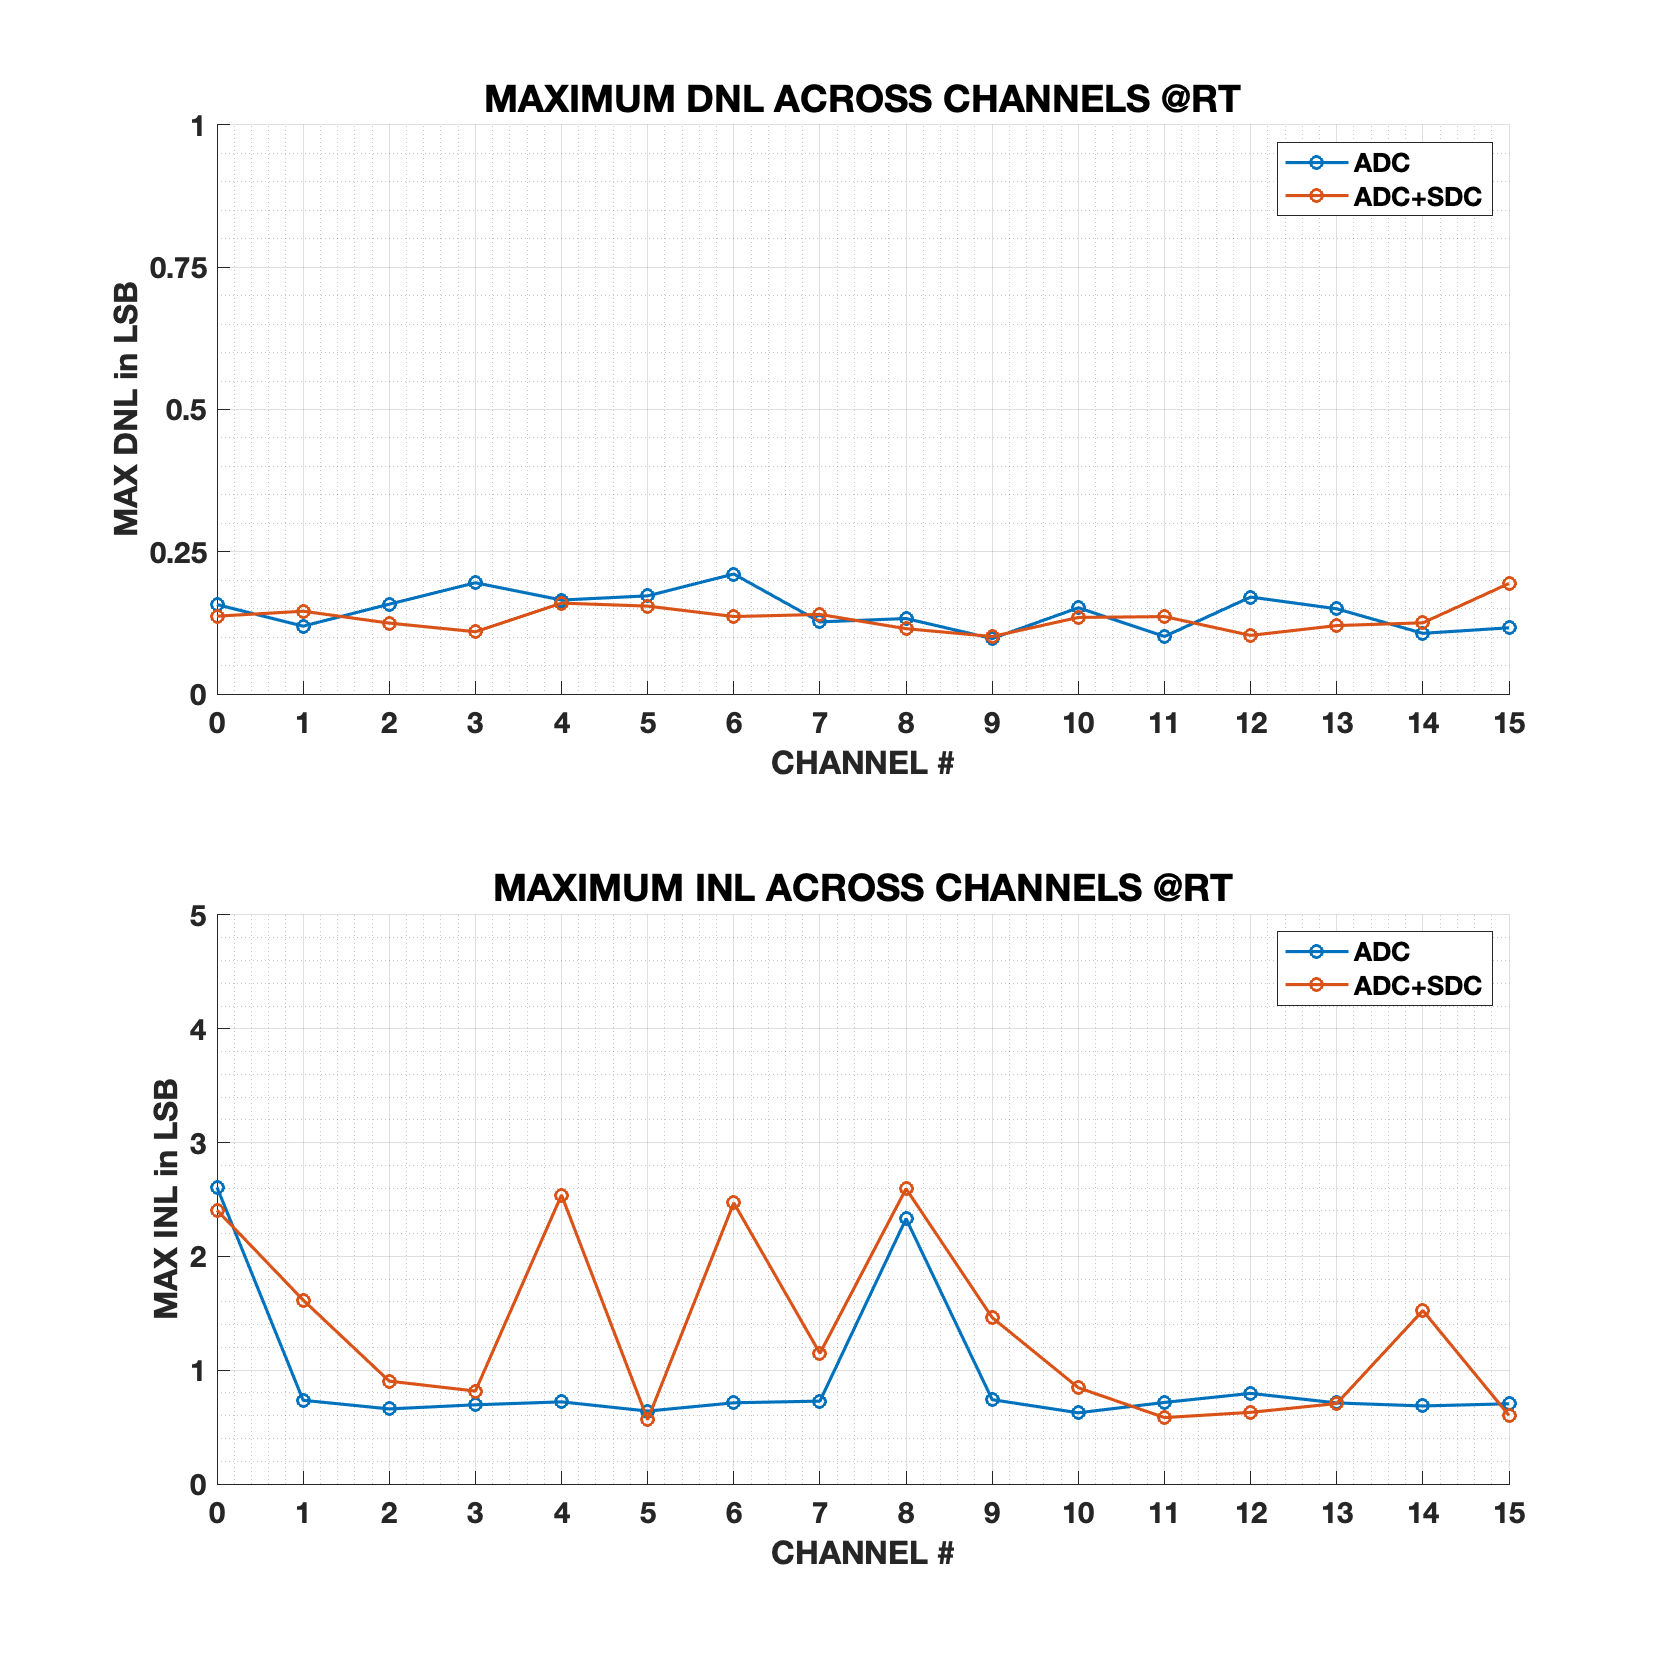
\includegraphics[width=1\linewidth]{figures/sdc_measurements/dnl_inl_ch_all_RT.png}
  \captionof{figure}{Maximum DNL and INL across ADC channels at room temperature.}
  \label{fig;sdc;inl_dnl_max_rt}
\end{minipage}
\hspace{0.2cm}
\begin{minipage}{.5\textwidth}
  \centering
  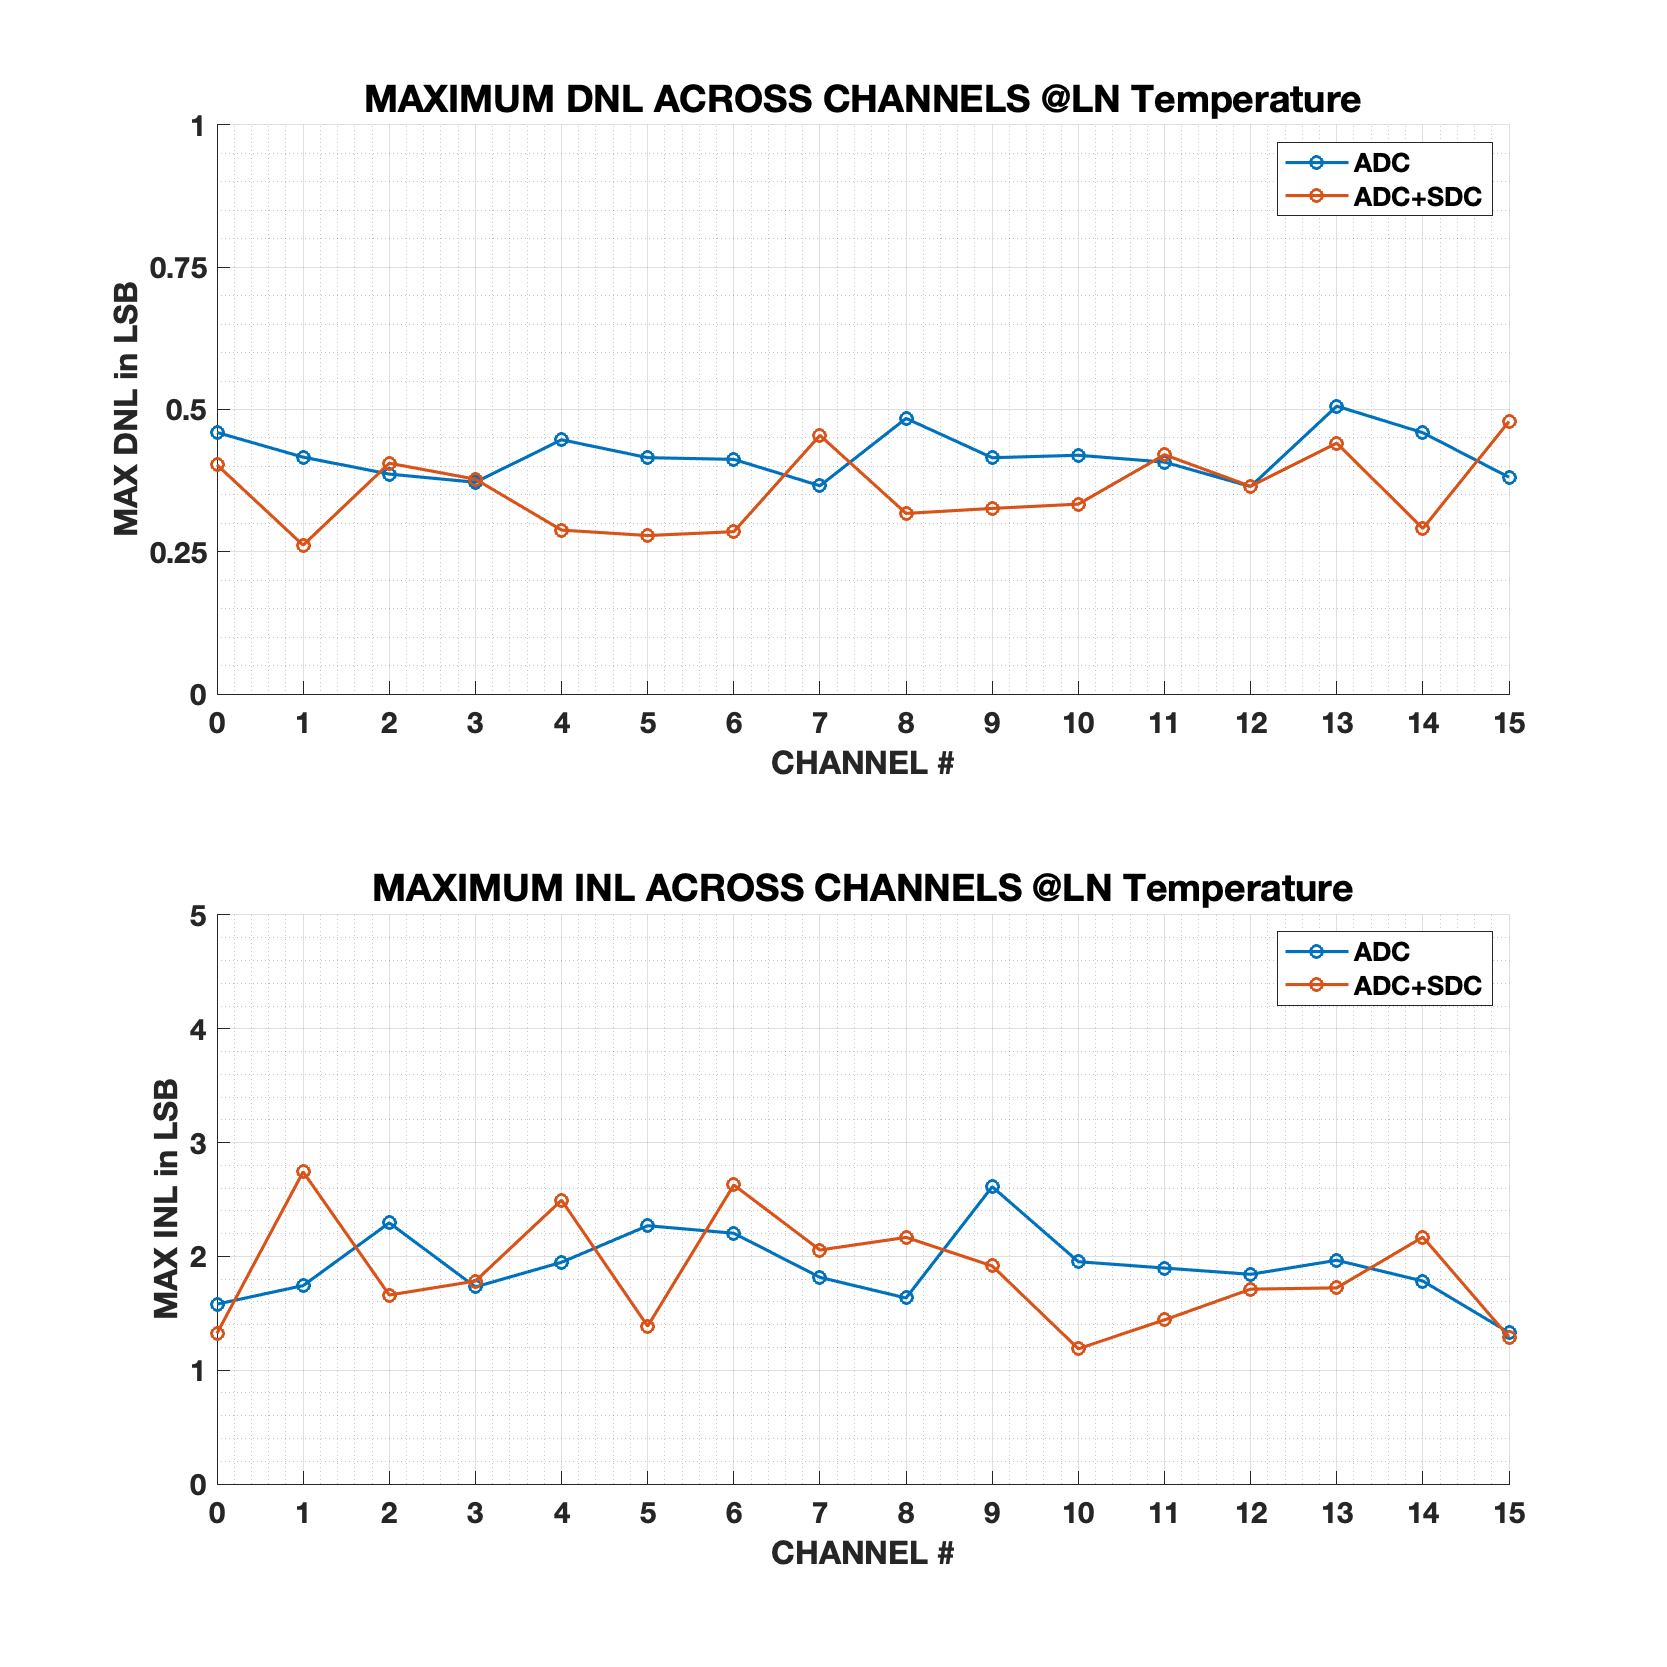
\includegraphics[width=1\linewidth]{figures/sdc_measurements/dnl_inl_ch_all_LN.png}
  \captionof{figure}{Maximum DNL and INL across ADC channels at liquid nitrogen temperature.}
  \label{fig;sdc;inl_dnl_max_ln}
\end{minipage}
\end{figure}

\begin{figure}[ht!]
  \centering
  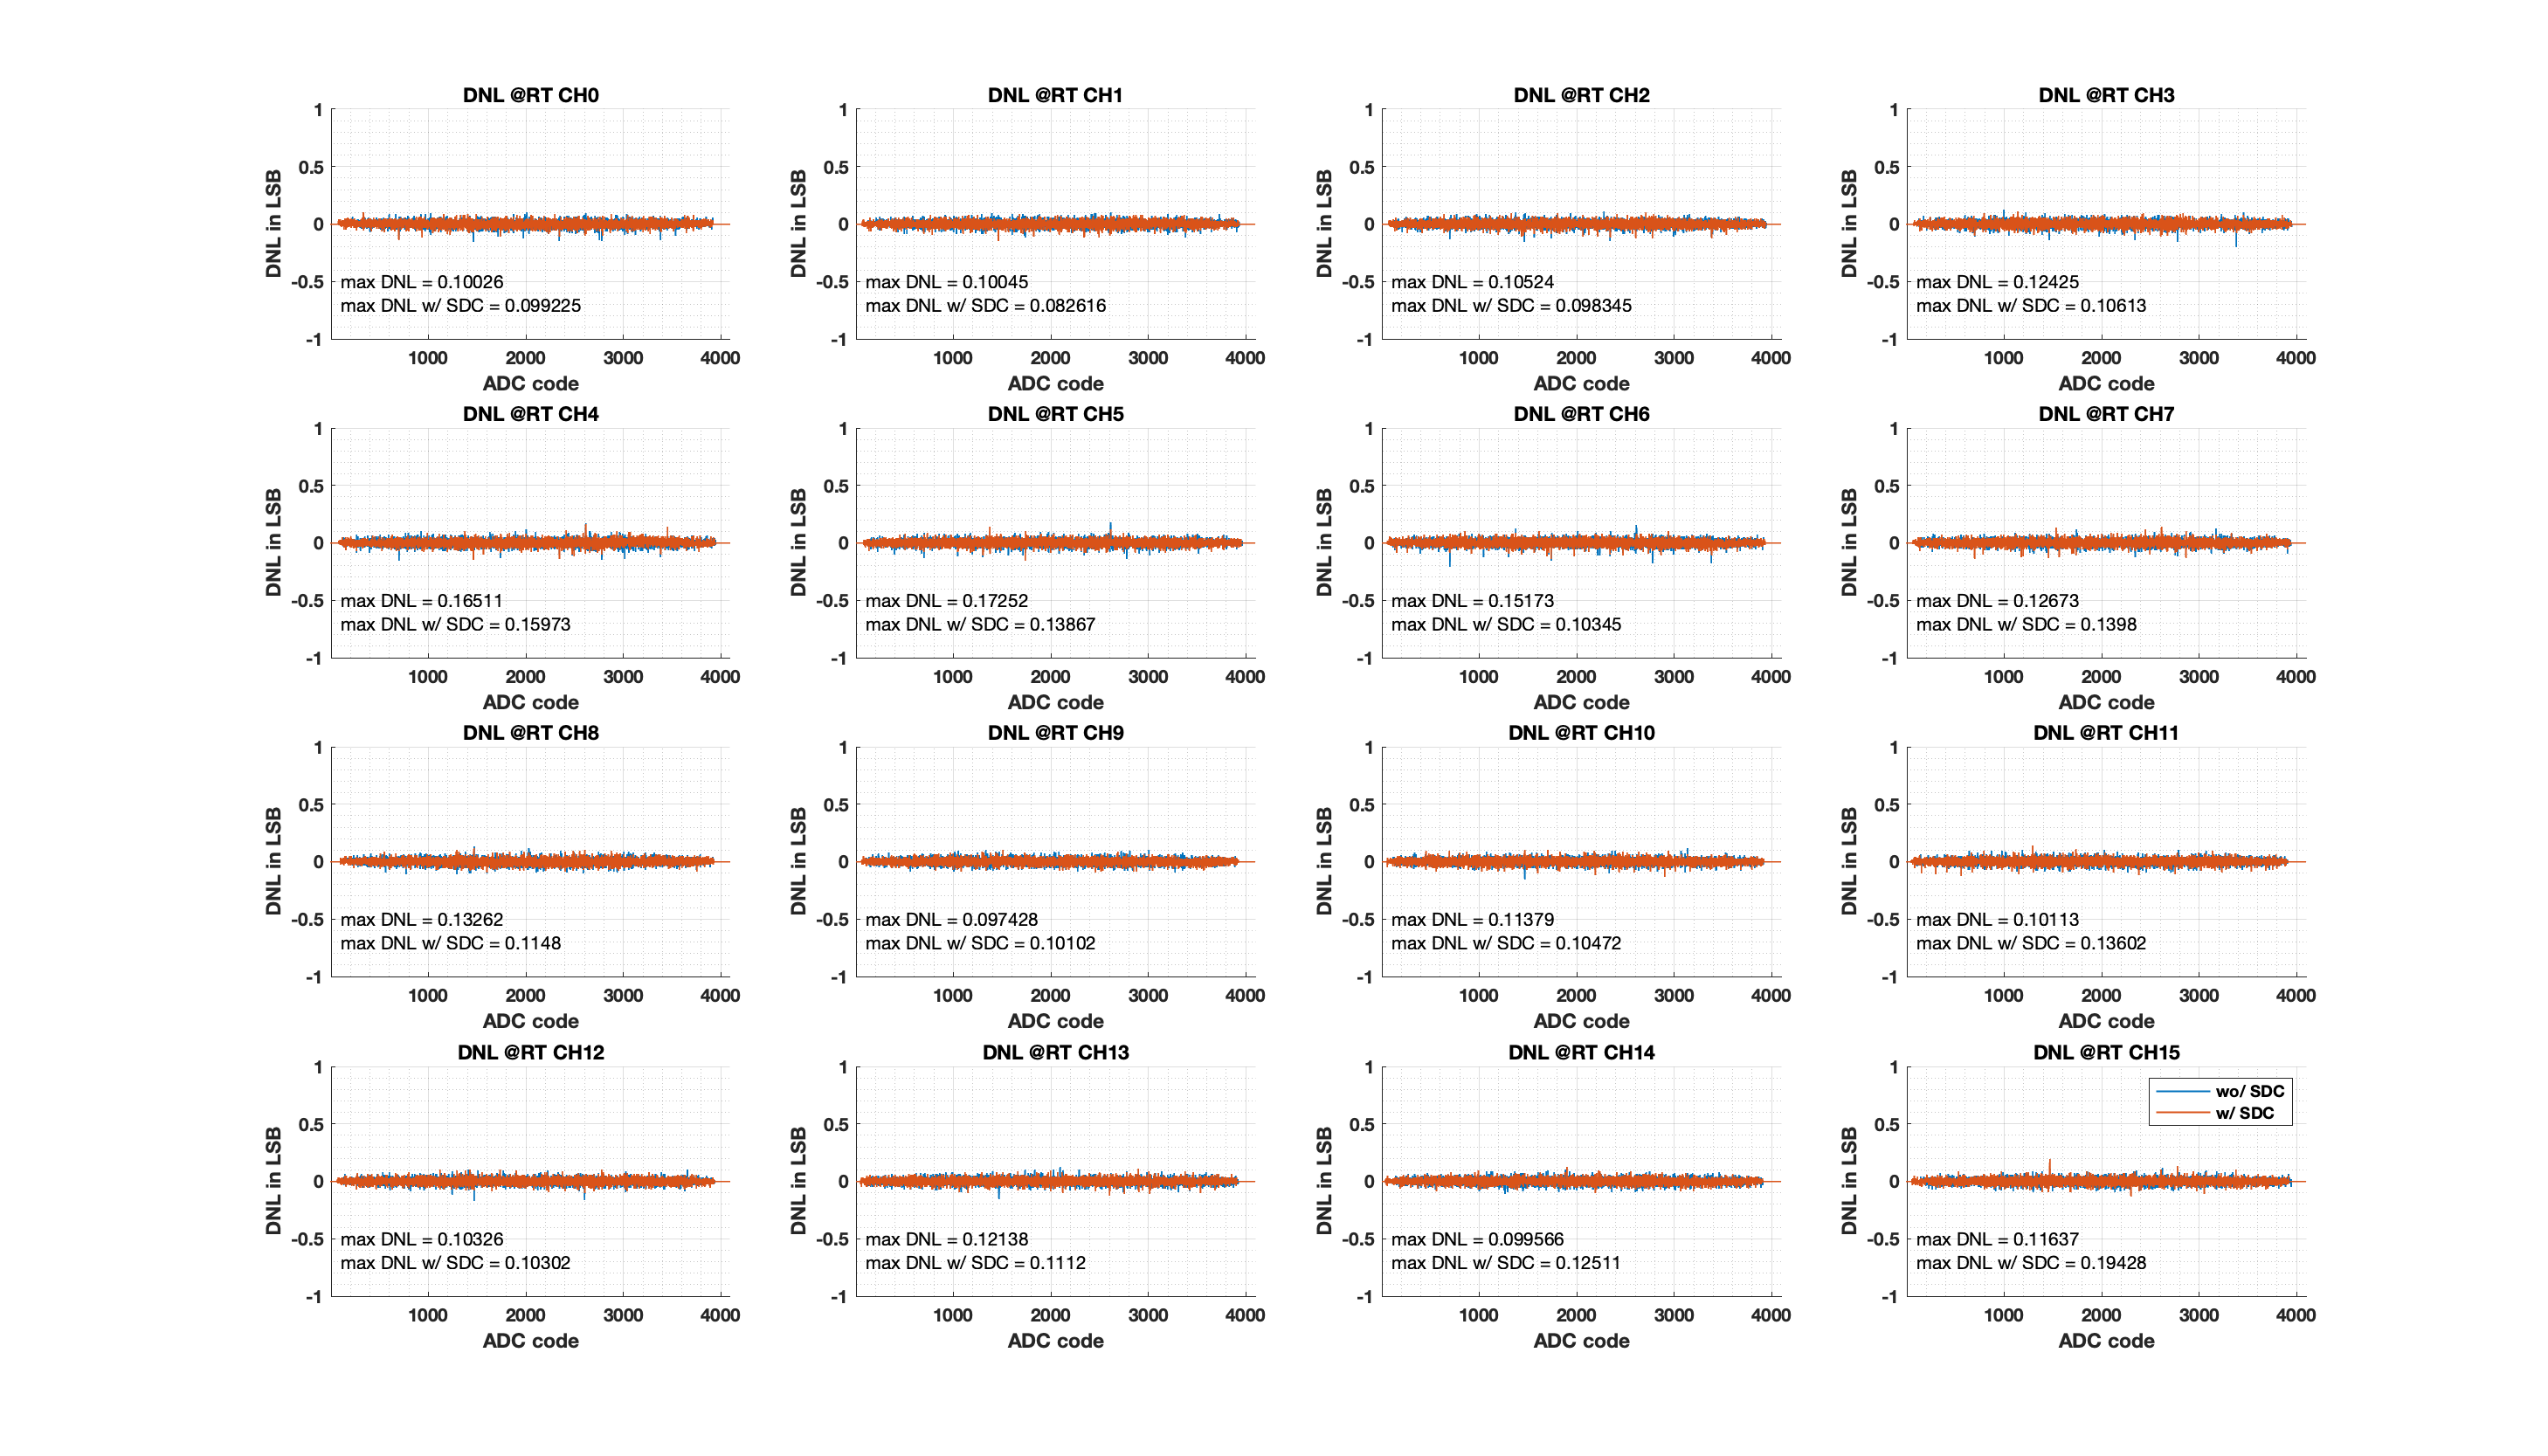
\includegraphics[width=1\linewidth]{figures/sdc_measurements/dnl_vs_dnl_sdc_all_ch_RT.png}
  \caption{Measurement of DNL across all ADC channels at room temperature. Blue - SDC off, Orange - SDC on.}
  \label{fig;sdc;dnl_all_rt}
\end{figure}

\begin{figure}[ht!]
  \centering
  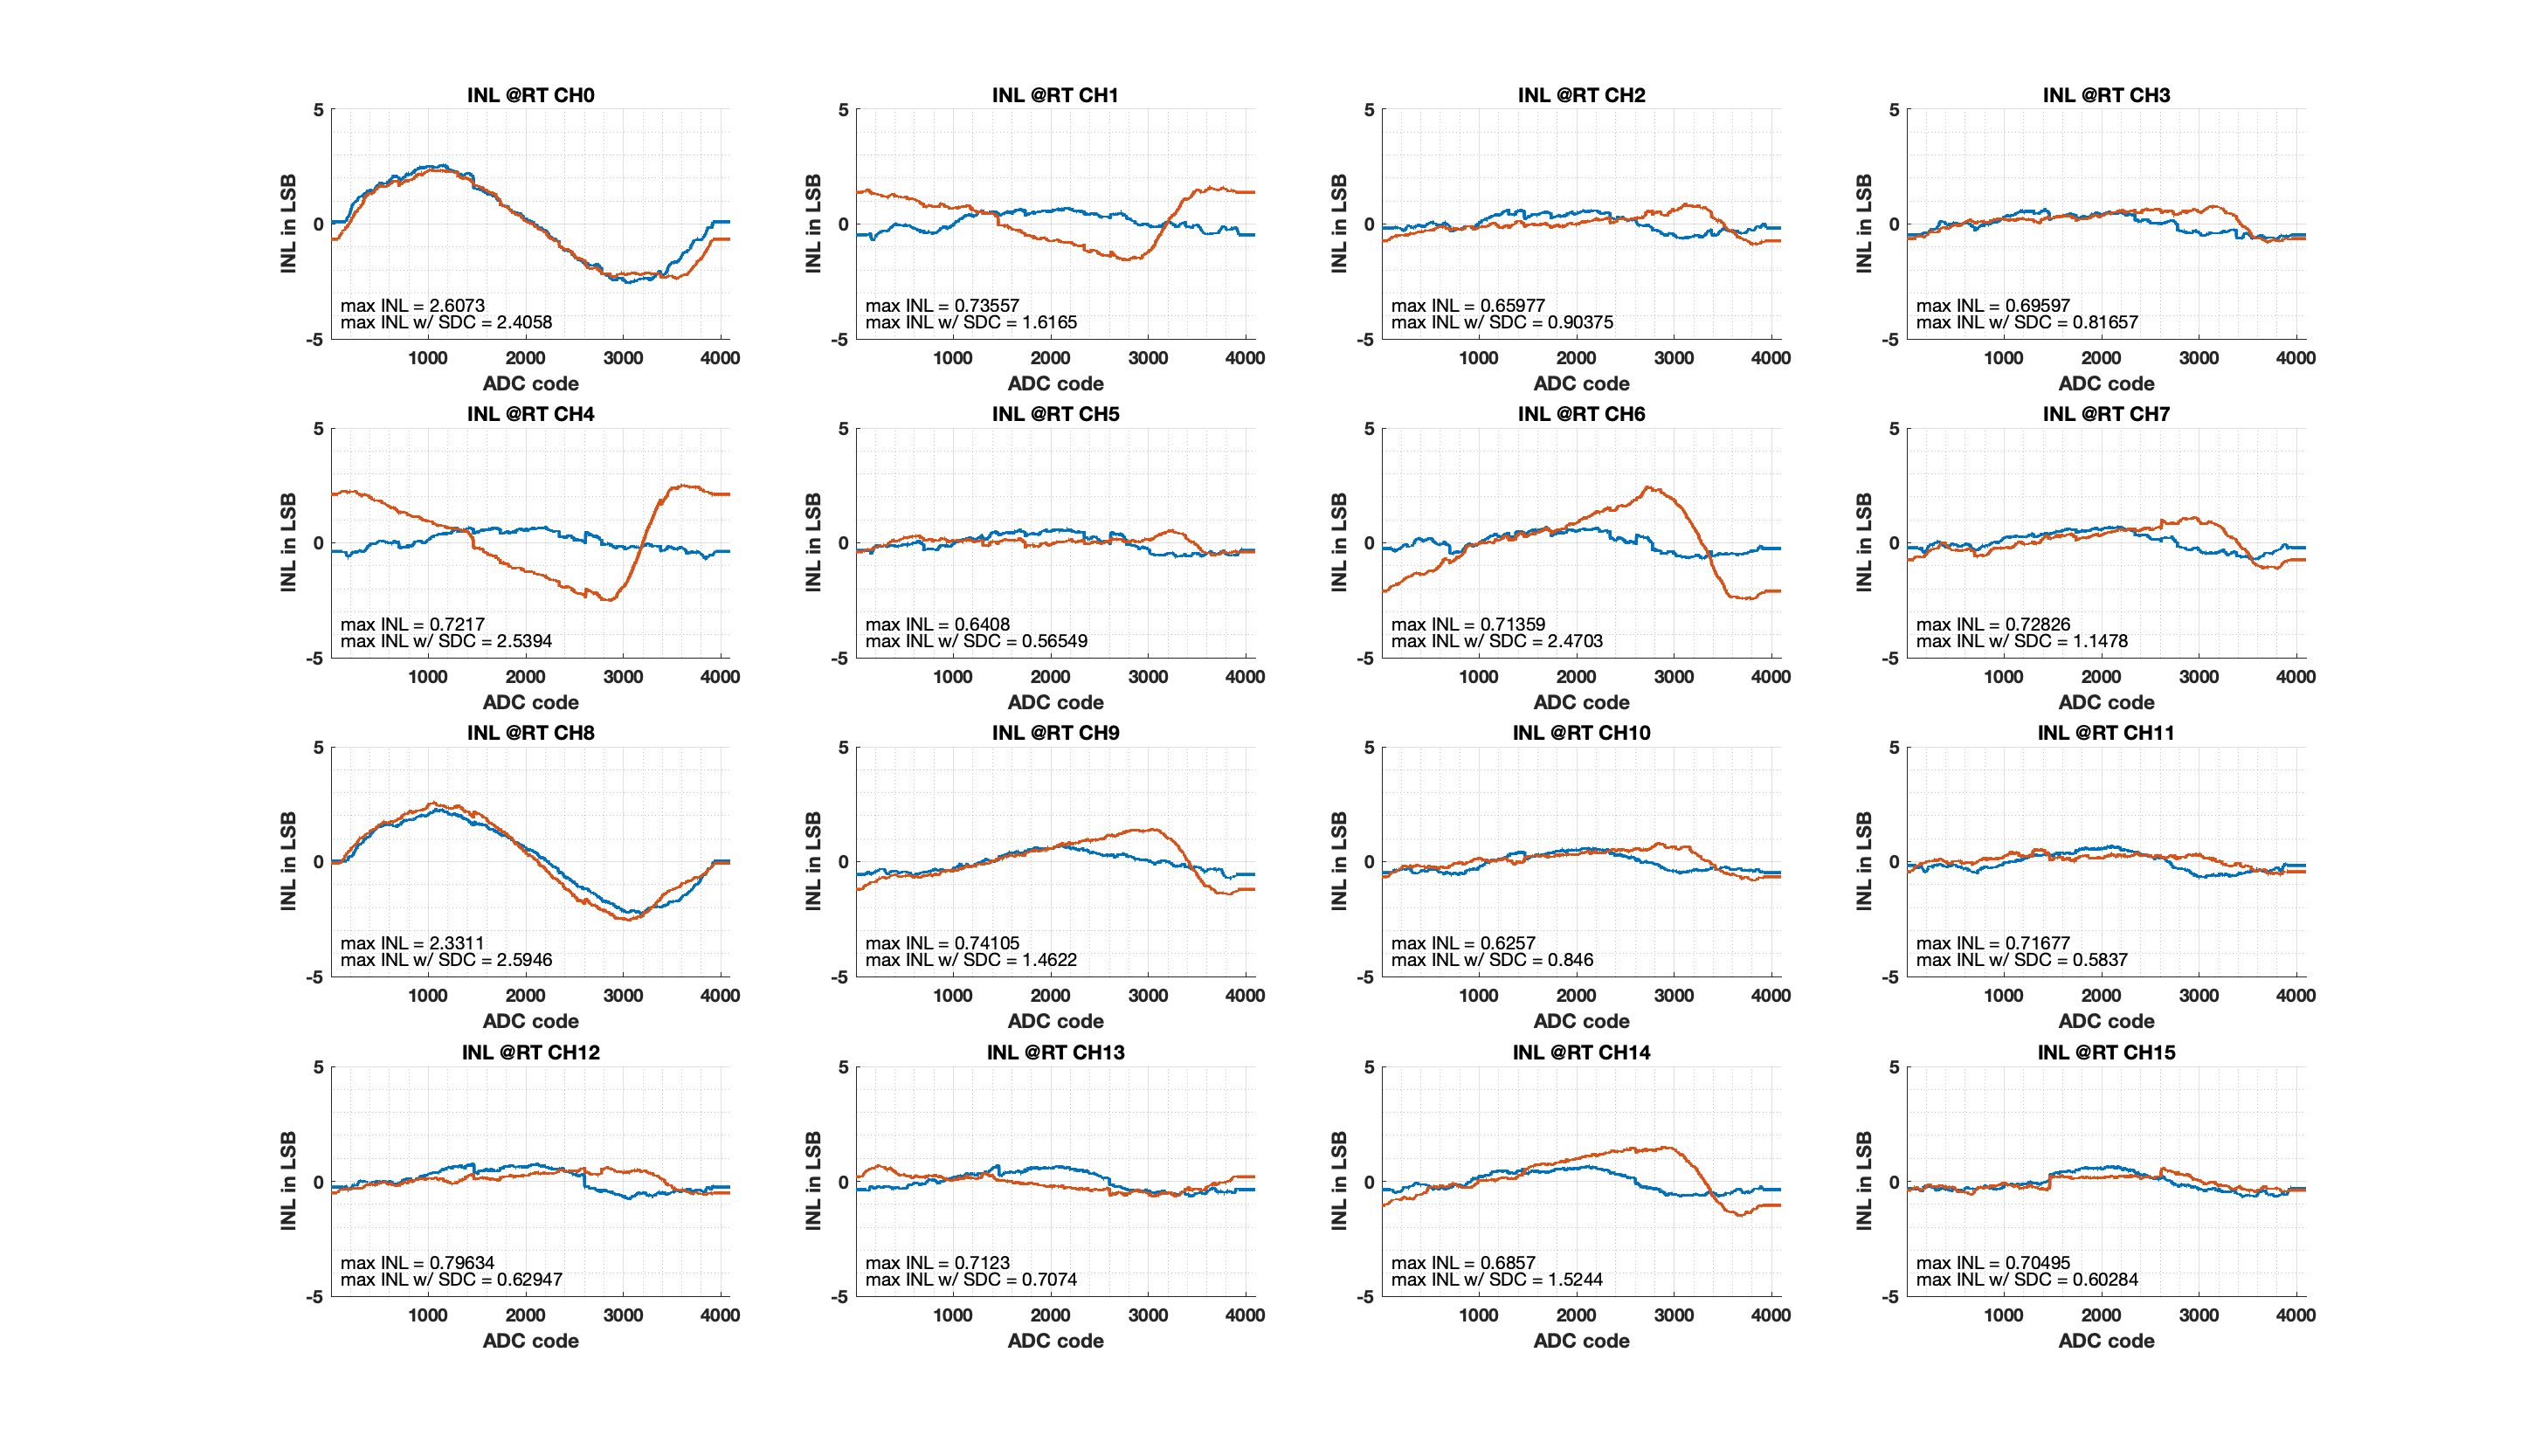
\includegraphics[width=1\linewidth]{figures/sdc_measurements/inl_vs_inl_sdc_all_ch_RT.png}
  \caption{Measurement of INL across all ADC channels at room temperature. Blue - SDC off, Orange - SDC on.}
  \label{fig;sdc;inl_all_rt}
\end{figure}

\begin{figure}[ht!]
  \centering
  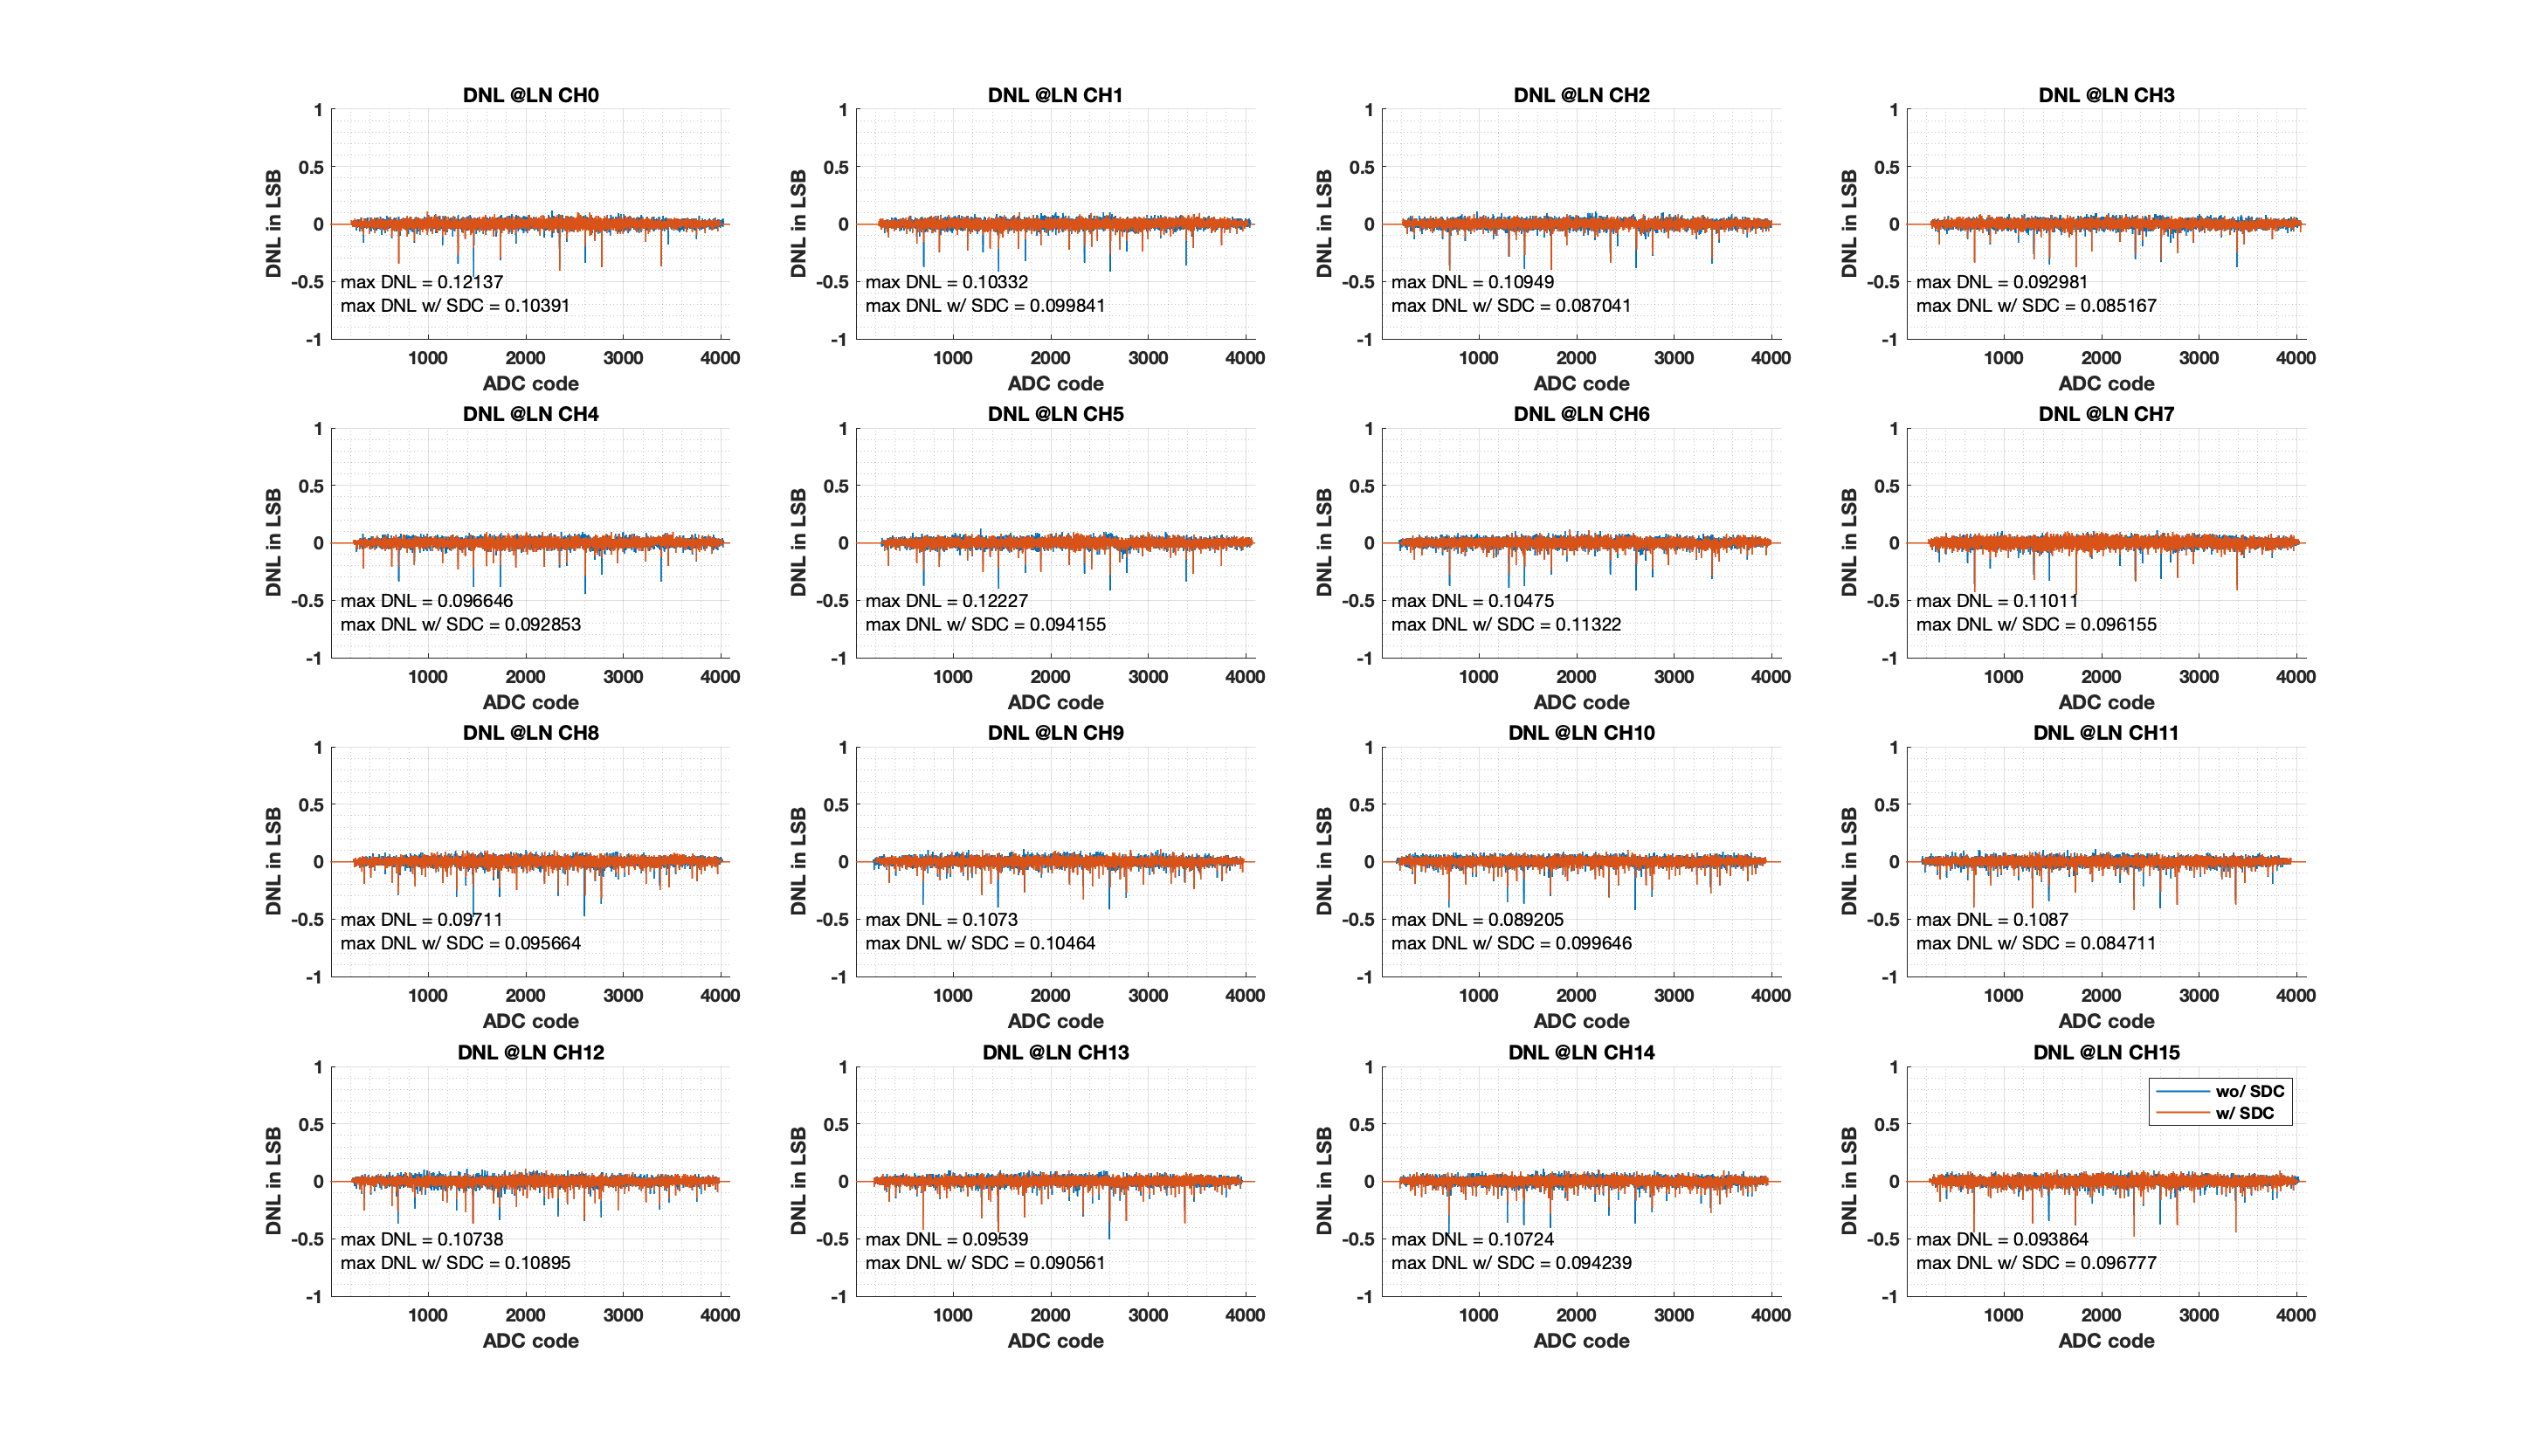
\includegraphics[width=1\linewidth]{figures/sdc_measurements/dnl_vs_dnl_sdc_all_ch_LN.png}
  \caption{Measurement of DNL across all ADC channels at liquid nitrogen temperature. Blue - SDC off, Orange - SDC on.}
  \label{fig;sdc;dnl_all_ln}
\end{figure}

\begin{figure}[ht!]
  \centering
  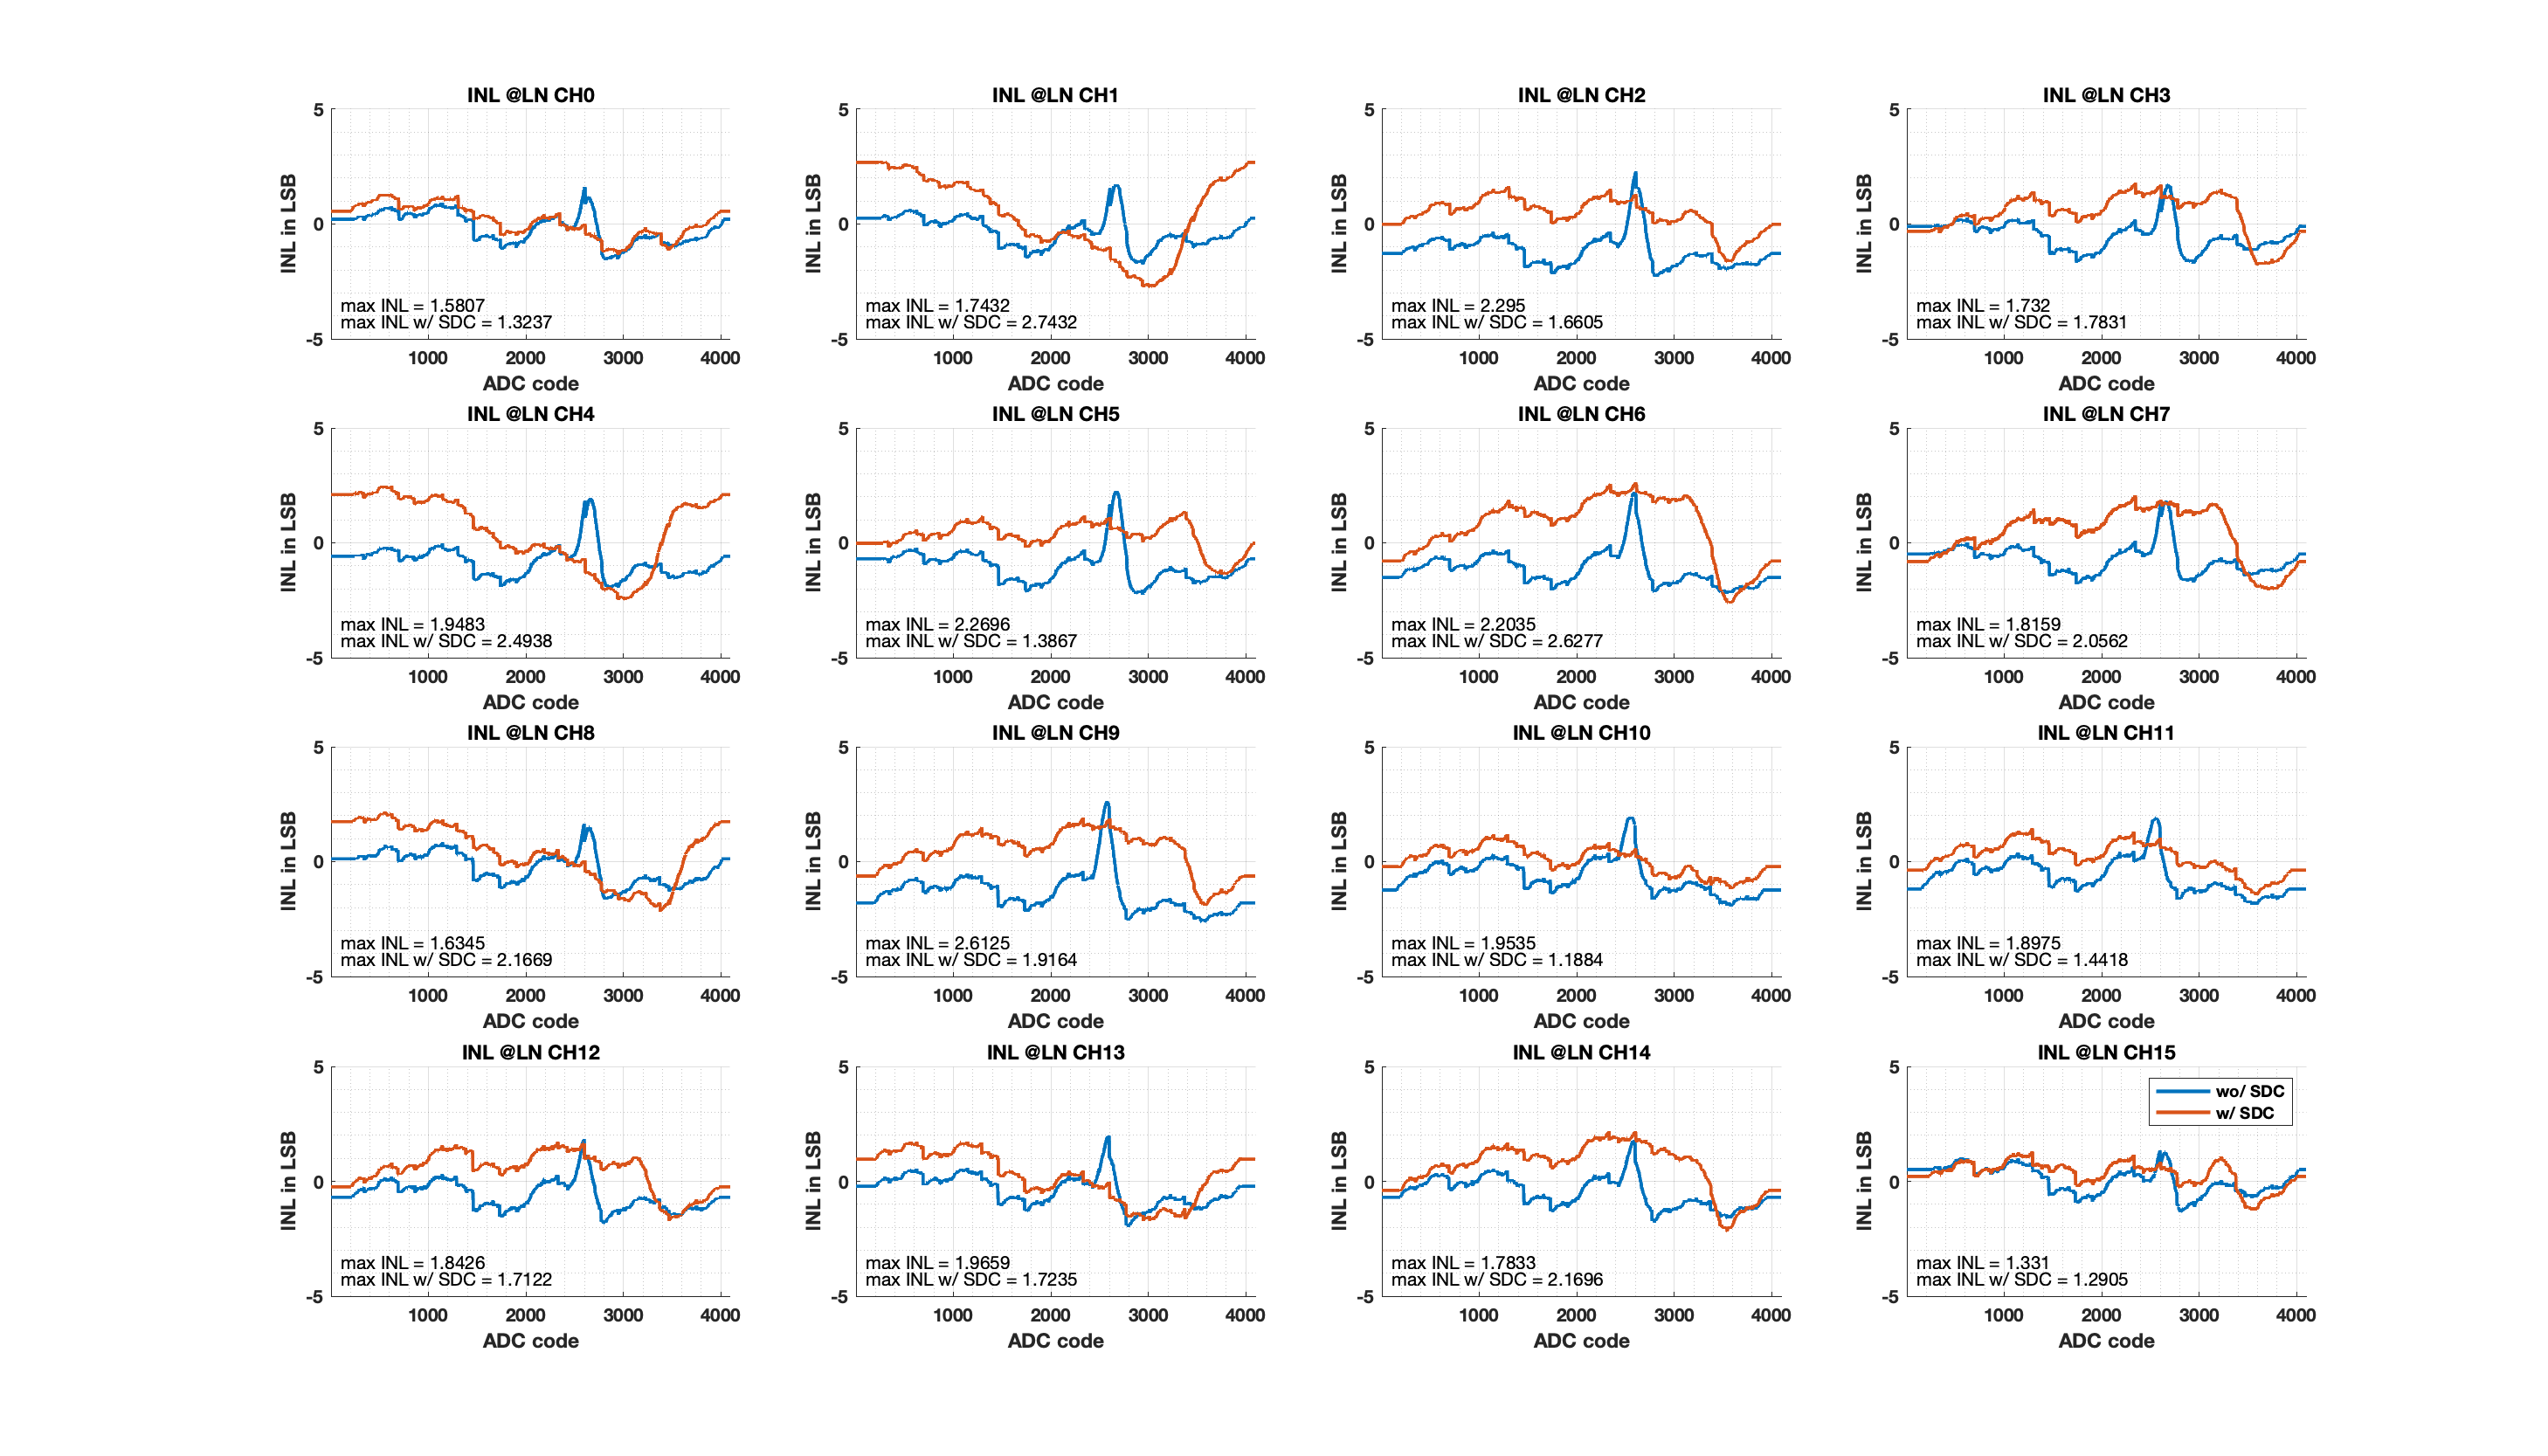
\includegraphics[width=1\linewidth]{figures/sdc_measurements/inl_vs_inl_sdc_all_ch_LN.png}
  \caption{Measurement of INL across all ADC channels at liquid nitrogen temperature. Blue - SDC off, Orange - SDC on.}
  \label{fig;sdc;inl_all_ln}
\end{figure}

\begin{figure}[ht!]
  \centering
  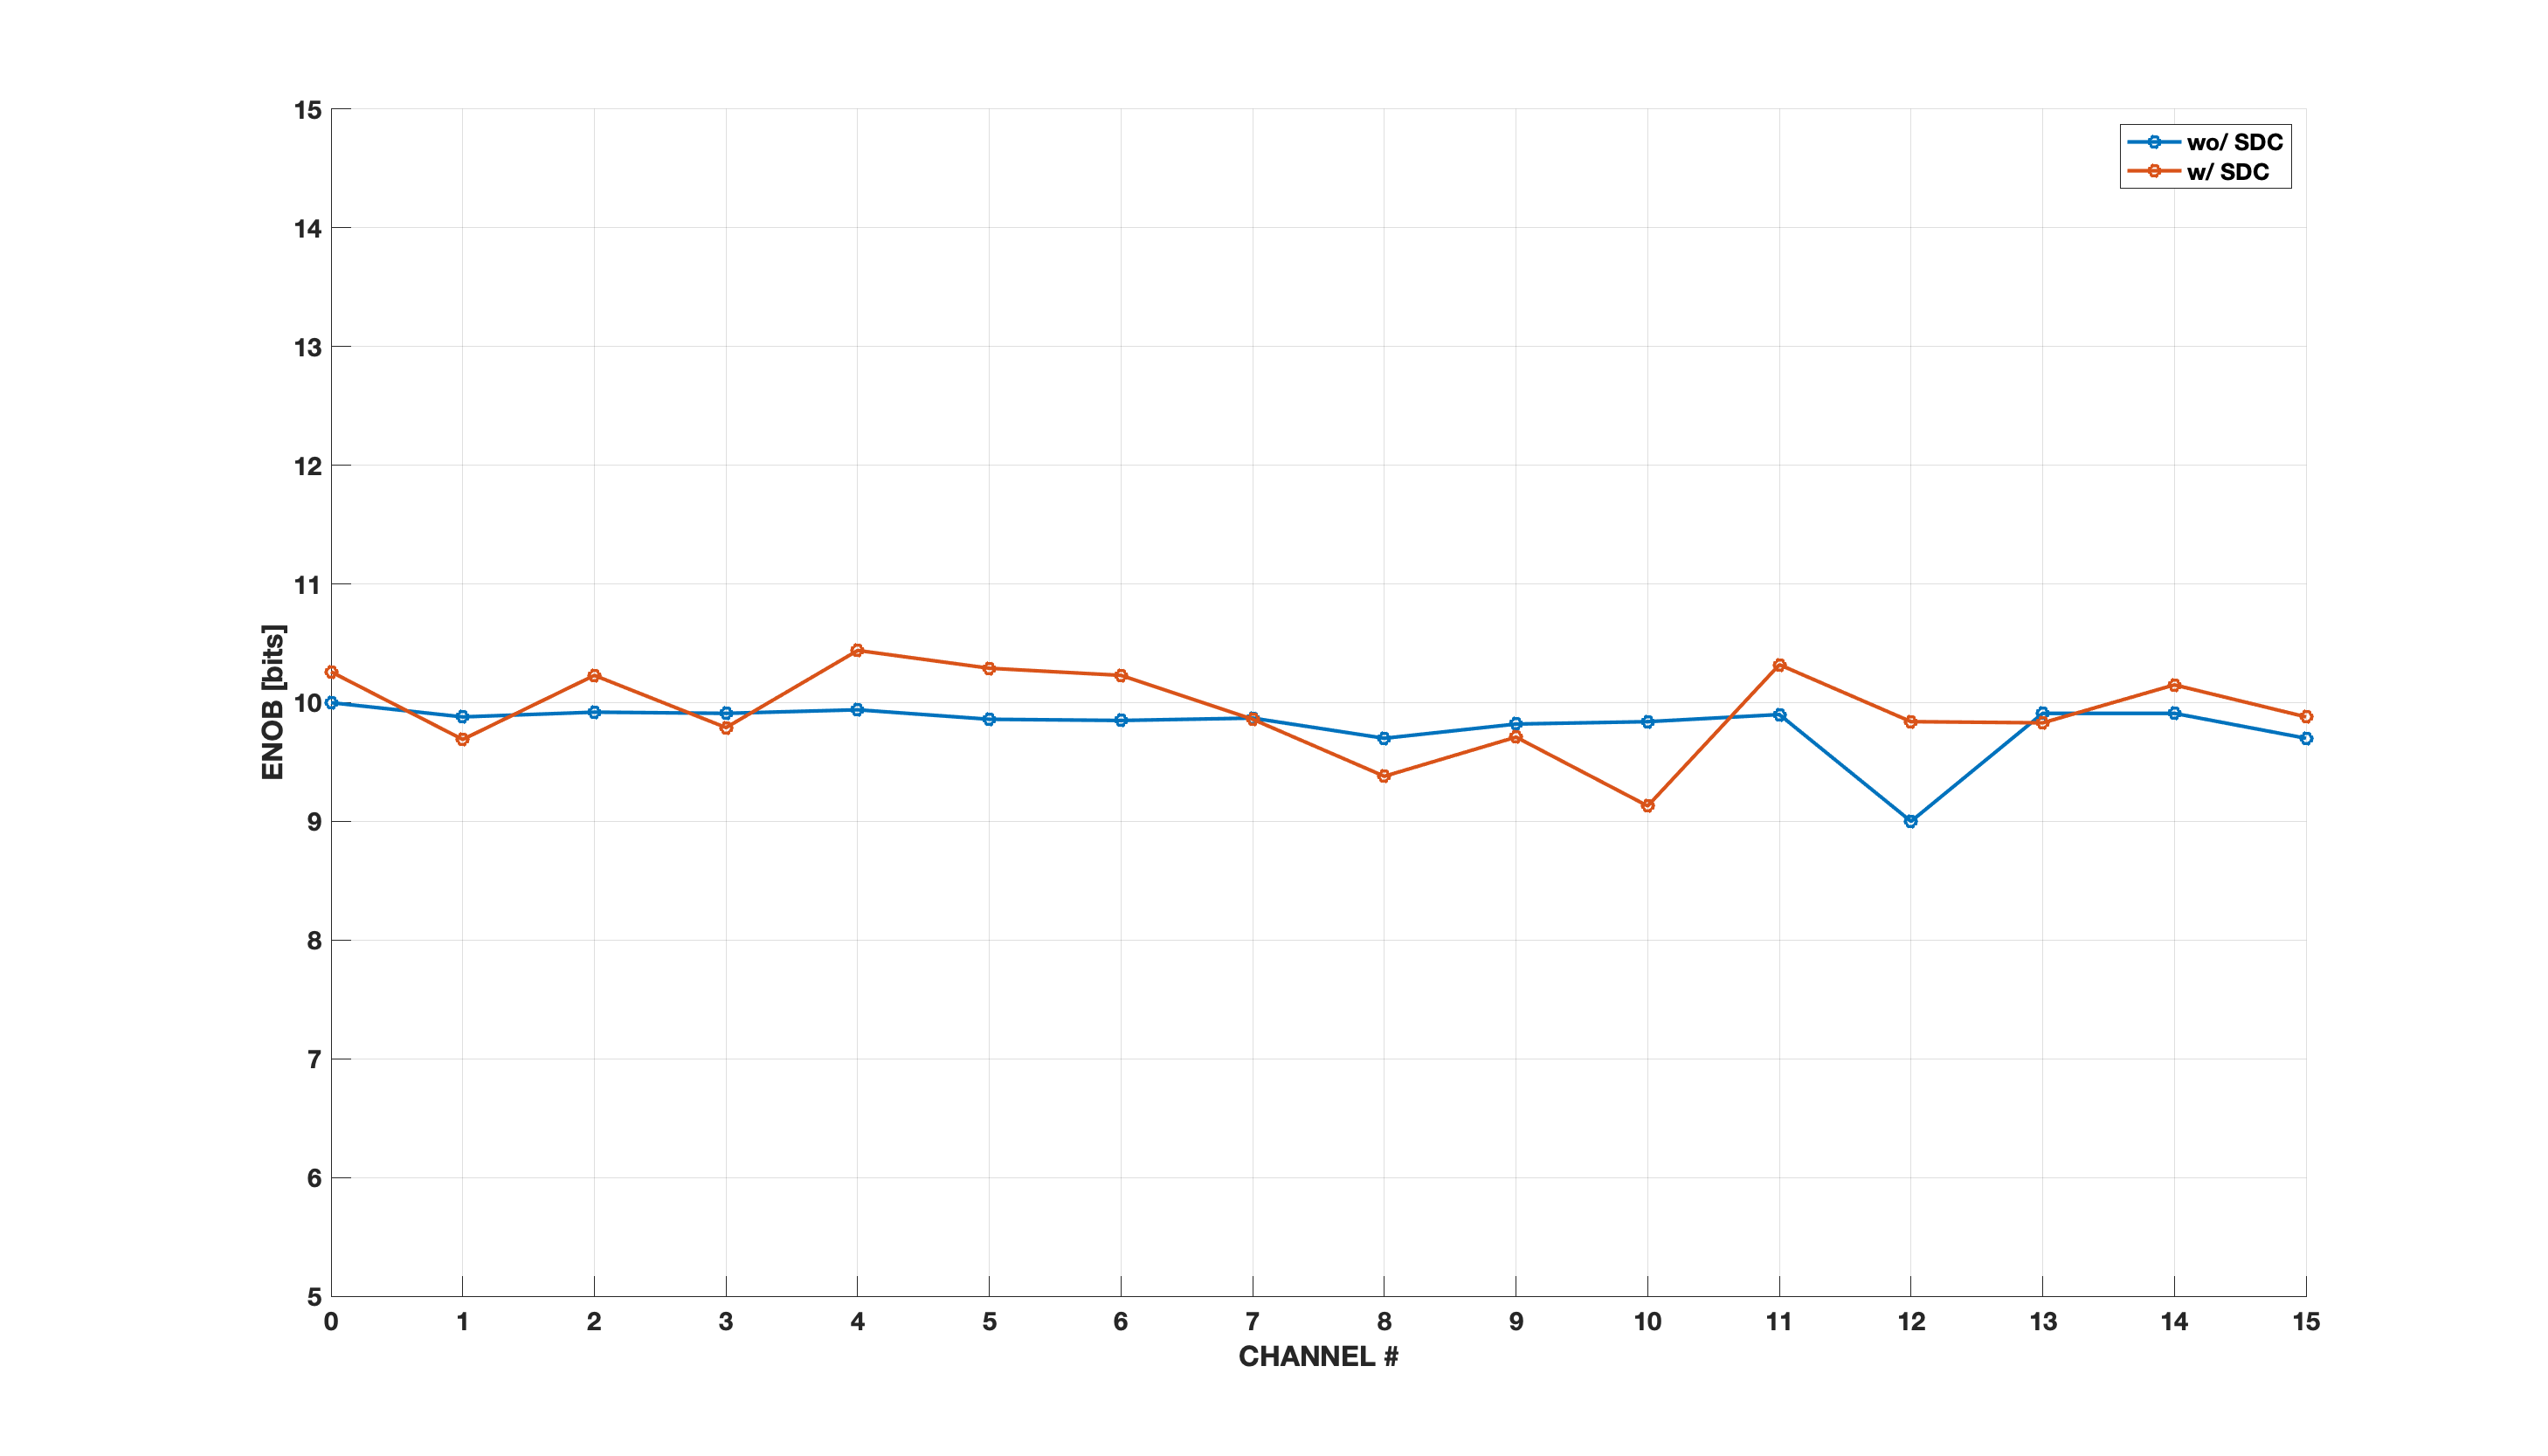
\includegraphics[width=1\linewidth]{figures/sdc_measurements/enob_rt.png}
  \caption{Measurement of ENOB across all ADC channels at room temperature.}
  \label{fig;sdc;enob_rt}
\end{figure}

\newpage
\clearpage

\clearpage
\newpage
\subsection{IR Drop }
\label{sec:5.6}

%%%%%%%%%%%%%%%%%%%%%%%%%%%%%%%%%%%%%%%%%%%%%%%%%%%%%%%%%%%%
%
% IR Drop
%
%%%%%%%%%%%%%%%%%%%%%%%%%%%%%%%%%%%%%%%%%%%%%%%%%%%%%%%%%%%%

At room temperature, when the test inputs are used to test the pipeline ADCs individually (bypassing the input buffers, Sample and Hold Amplifiers (SHAs), and the SHA multiplexer), significant non-linearity is observed for input signals near the voltage extremes of the ADC.  At cryogenic temperature, no significant deviation from linearity is observed.  We interpret this as evidence that there is an IR drop on the analog 2.5V power when the chip is operated at room temperature.  The fact that the non-linearity is not observed at cryogenic temperature is consistent with the fact that the resistivity of the metal used to distribute the power is greatly reduced at cryogenic temperature. 
Metal layers M8 and M9 were used for power distribution.  The redistribution layer (AP) was not used and could easily be added to the power mesh in the analog sections of COLDADC.  We will make this change in the next submission.
\subsection{SHA/MUX Crosstalk }
\label{sec:5.7}

%%%%%%%%%%%%%%%%%%%%%%%%%%%%%%%%%%%%%%%%%%%%%%%%%%%
% Channel crosstalk
%%%%%%%%%%%%%%%%%%%%%%%%%%%%%%%%%%%%%%%%%%%%%%%%%%%

While there is no formal specification regarding the channel crosstalk, we have measured crosstalk of $<0.5\%$ in LN$_2$ and $<1\%$ at RT. We have done a variety of measurements that suggest the crosstalk is due to kickback between the channels during the sampling phase that makes it so the SHAs are not completely settled between samples. When the channels are slowed down, the crosstalk is somewhat mitigated, which indicates that it is due to insufficient bandwidth in the SHA MUX. To improve this, we will lower the impedance of the MUX to allow faster settling.

\subsection{Bandgap Voltage Reference (BGR) Op-Amp }
\label{sec:5.8}

%%%%%%%%%%%%%%%%%%%%%%%% 
% (DABROWSKI) BGR Op-amp
% Grace's version
%%%%%%%%%%%%%%%%%%%%%%%%%
To operate correctly, the ColdADC requires accurate voltage references for the ADC. In addition, the various analog circuits on the prototype require bias currents. To mitigate risk, the ColdADC includes two redundant reference generation blocks to supply these needed voltages and currents, one block based on a bandgap reference, and one based on a CMOS reference. 

A voltage proportional to the bandgap of silicon is generated in the V-BGR core. This voltage is then converted to a current in the I-DAC block to generate bias currents. In addition, the bandgap voltage is scaled by the various V-DAC blocks. Because the reference voltages for the ADC span a significant portion available power supply voltage, two different versions of the V-DAC are required: one to generate voltages near the supply voltage, and one to generate voltages near ground. Unfortunately, the wrong version of the V-DAC was included to generate VREFP (a voltage near the supply is required, but the included V-DAC is the version intended for voltages near ground). The included V-DAC can still generate the required voltage for VREFP if it is given significant additional headroom, in other words if VDDA is elevated above nominal.

While the BJT-based reference is fully functional in this case, it is not appropriate for long-term reliability because the supply should be operated below nominal, not above. The fix for this design error is simple: replace the VDAC that generates VREFP with the appropriate version of the V-DAC.


\subsection{Overflow Wraparound }
\label{sec:5.9}

%%%%%%%%%%%%%%%%%%%%%%%%%%%%%%%%%%%%%%%%%%%%%%%%%%%
% Overflow wraparound
%%%%%%%%%%%%%%%%%%%%%%%%%%%%%%%%%%%%%%%%%%%%%%%%%%%

The gains of each stage are weighted by the calibration. If the sum of the weights of the stages is greater than $2^{16}$, then the digital correction logic can overflow, and a large input can lead to a small output code and vice versa. The stages were designed with an analog closed-loop gain slightly less than two. Based on supplied process data, we expected the closed-loop gain would be low enough to be free from overflow. In fact this was not the case and overflow was observed when the input voltage was close to one of the reference voltages. This can be seen in Figure~\ref{fig:adcoverflow}, which shows the response of the two different ADCs on one of the ColdADC prototypes to the same input signal. The left portion of Figure~\ref{fig:adcoverflow} shows the ramp response of ADC0 and the prototype operates as expected. When the ADC is saturated, the digital output is pinned to its maximum value. On the right portion of Figure~\ref{fig:adcoverflow} overflow is observed as part of the ramp response of ADC1. In this case, the ADC input reaches its maximum value but instead of remaining pinned, the digital output jumps to a low value. This is due to higher-than-expected closed-loop gain in ADC1.
\begin{figure}[htb]
\centering
%\begin{minipage}[b]{1.0\textwidth}
\begin{center}
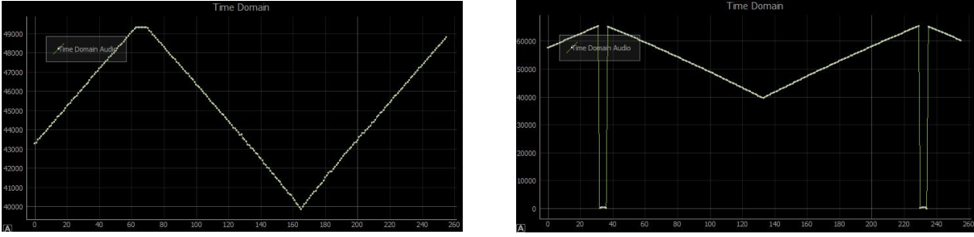
\includegraphics[width=1.0\textwidth]{figures/ADCOverflow.png}
\end{center}
%\end{minipage}
\caption{Digital overflow. The image on the left corresponds to ADC0 and the image on the right corresponds to ADC1.}
\label{fig:adcoverflow}
\end{figure}

We will fix this in two ways. First, we will further reduce the analog gain of the stages. Second, we will add to the next version of the prototype a digital overflow detection block that will sense over (or under) flow and pin the output code at a high or low level, respectively. It will do that by looking at the sign bit of the running sum one stage prior to the last. Then the algorithm will know whether to pin to a high or low value.

%%%%%%%%%%%%%%%%%%%%%%%%%%%%%%%%%%%%%%%%%%%%%%%%%%%
\clearpage
\newpage
\section{Production Testing }
\label{sec:6}

%%%%%%%%%%%%%%%%%%%%%%%%%%%%% 
% (FURIC) Production Testing
%%%%%%%%%%%%%%%%%%%%%%%%%%%%%

A Production Test Site is currently being assembled at the Univeristy of Florida to perform QC of all the packaged ColdADC ASIC.  The production QC procedure was developed and tested on the first 33 packaged chips at BNL. In this section, we describe the production test system and the results from the first 33 chips.

\subsection{Test Setup}
\label{sec:6.1}
The ColdADC QC teststand is a dedicated system to characterize the ColdADC performance with a low distortion 
signal generator SRS DS360, which is very similar to the test setup described in Section~\ref{sec:2.2}.  
Shown in Figure~\ref{fig:prodQC_blockdiagram} is the block diagram of the setup. The testboard has an ASIC 
socket mezzanine card to avoid having to solder the ColdADC chips. 
This convenience, however, introduces additional capacitance from the ASIC socket which may slightly degrade the test results.
Since the main purpose of the production testing is to distinguish good chips from bad chips, the performance degradation 
from the additional capacitance is not an issue. 
Instead of an on-board oscillator to provide 100MHz clock for FPGA Mezzanine, an external clock source SRS CG635 is used to provide a 
stable clock for both room temperature and liquid nitrogen operations. For ENOB/FFT measurements, clock synchronization between the 
board and the signal generator is required.  Without an external clock source it can be difficult to obtain a stable synchronization 
between the testboard and the signal generator. 
%In fact, for internal ADC core measurements (8 MHz Nyquist bandwidth), 
%unwanted spikes at 2 MHz and 6 MHz can appear at cold. This issue is strongly mitigated by adding an external clean clock source. 
%So, the teststand is updated with the CG635 generator sends a 100 MHz clock to the board and a 10 MHz synchronized signal to the DS360. 
%Figure 2 shows the test setup at room temperature while Figure 3 shows the test setup at LN2 temperature
\begin{figure}[h!]
\centering
  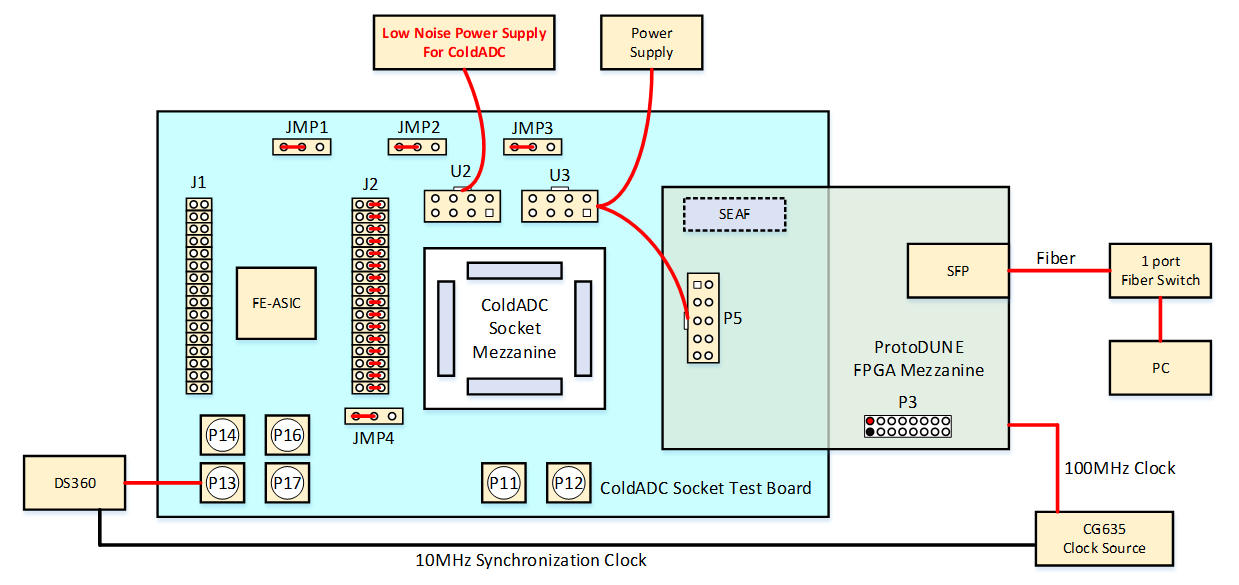
\includegraphics[width=0.8\linewidth]{figures/prodQC_blockdiagram.png}
  \caption{Block diagram of ColdADC Production Testing setup.}
  \label{fig:prodQC_blockdiagram}
\end{figure}

The flowchart of the QC process is shown Figure~\ref{fig:qc_flowchart}.  The chart illustrates the sequence of steps for characterizing 
the functionality and performance of the chip. At every iteration, the measurements is done using BJT reference and then repeated 
again using the CMOS reference. 
%With a certain number of tested chips, it will be possible to highlight differences in performance between measurements taken 
%using one reference instead of the other. 
%The test flow includes input configuration, initialization checkout, static linearity (INL/DNL per channel), 
%Dynamic Behavior (ENOB/SFDR/SINAD per channel), DC noise per channel, and ADC core characterization. 
The list below describes the QC steps in more detail: 
\begin{enumerate}
\item Input configuration: ColdADC chip ID and test board ID are recorded, the path for data storage is specified. 
\item Initialization checkout: mainly to check ColdADC functionality. It includes power consumption with different 
configurations, power cycles, I2C/UART communication check, pattern and register check, reference sweeping check, 
synchronization and calibration check. Any chip failed in any procedure in this checkout is treated as a bad chip. 
\item  Static linearity: INL/DNL results are obtained with a sine wave input from the DS360 generator. Data and plots 
are generated with the sine wave code-density method. Performances at both 2 MS/s/ch and 500 kS/s/ch are measured.
\item Dynamic Behavior: ENOB/SFDR/SINAD is calculated from the FFT plot obtained by using coherent sampling. 
Performances at both 2 MS/s/ch and 500 kS/s/ch are measured. 
\item DC noise: Two DC points, 200mV and 900mV are chosen.
\item ADC core characterization (optional): DNL/INL, FFT, and DC noise. 
\end{enumerate}

The test procedure is largely automated using Python scripts. The only step that requires manual intervention is to replace the ASIC chips 
at the end of the measurement. When the test is completed, the Python script automatically generates a detailed report in pdf format. 
The report includes:
\begin{enumerate}
\item Summary: date and time, temperature, chip and board IDs, power consumption and characterization results (CMOS reference only, can be changed to BJT);
\item Initialization checkout: ADC power consumption with both BJT and CMOS references, sweep plots of reference voltages and currents;
\item Calibration weights: recorded weights listed with respect to internal ADC stages;
\item Noise study: RMS noise for each channel and comparison between all channels. Four pages in total: 200 mV and 900 mV baselines for both BJT and CMOS references;
\item Channels characterization: noise, linearity and dynamic studies, with both BJT and CMOS references for comparison. Each page collects results for one channel;
\item ADC test input: internal ADC characterization for two sampling rates, 4 MS/s and 16 MS/s.
\end{enumerate}
\begin{figure}[h!]
\centering
  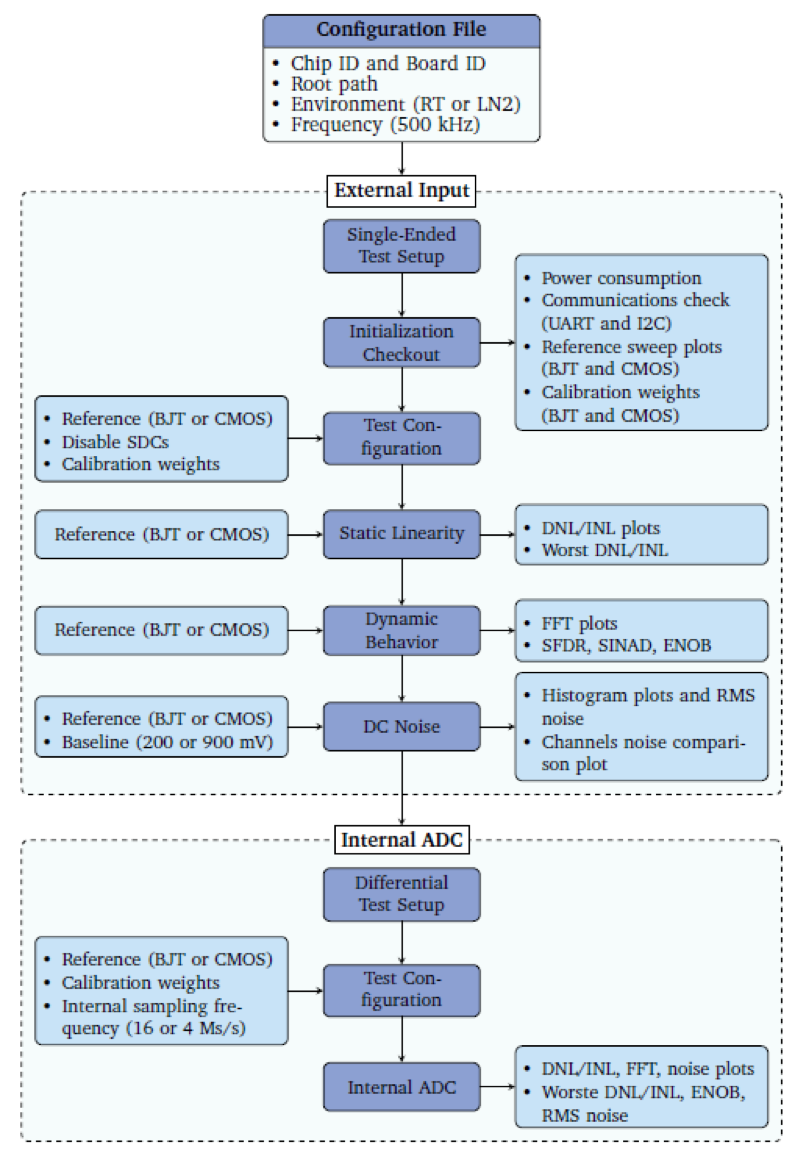
\includegraphics[width=0.8\linewidth]{figures/QC_flowchart.png}
  \caption{ColdADC QC Flowchart.}
  \label{fig:qc_flowchart}
\end{figure}

At the moment, the test data are stored in a local database at BNL. U. of Florida group is developing an online database for the ColdADC QC test that will be used for all future production tests.
%Ivan Furic research team from Florida University is going to develop an online database for the ColdADC QC test. BNL provides hardware, FPGA firmware, python scripts and necessary support to help them replicate the test procedure at BNL.  Florida University is responsible for QC test of 100 ColdADC chips in the coming two or three months. 

\subsection{Results}
\label{sec:6.2}
For the initial production QC test, a batch of 33 ColdADCs were tested. One of the chips (\#00096)  drew very high current (>1 A) when it 
was first powered and was excluded from further QC testing. It was found that the bad chip had a resistance of $<$ 5$\Omega$ between 
VDDA2P5 and VSSA2P5, while the nominal resistance should be about 12 k$\Omega$. The cause of the failure is not clear; may be due to 
manufacturing defect or handling issues. In additional to the 33 QC chips, 20 other chips were previously tested at BNL and passed 
functionality tests. Based on a sample of 53 chips (51 packaged and 2 bare dies), the functionality failure rate of ColdADC is less than 2\%.

\subsubsection{Power Consumption}
The power consumption of ColdADC strongly depends on the chip configuration. The power consumption with VDDA2P5/VDDD2P5=2.5V, 
VDDD1P2=2.1V, VDDIO=2.25V, SDC\&DB bypassed, CMOS reference, floating single-end input, and 2 MS/s sampling rate is summarized in in 
Figure~\ref{fig:qc_power}. For this configuration, the average power consumption of ColdADC is about 413 mW at room and 450 mW at LN$_2$ temperature.
\begin{figure}[h!]
\centering
  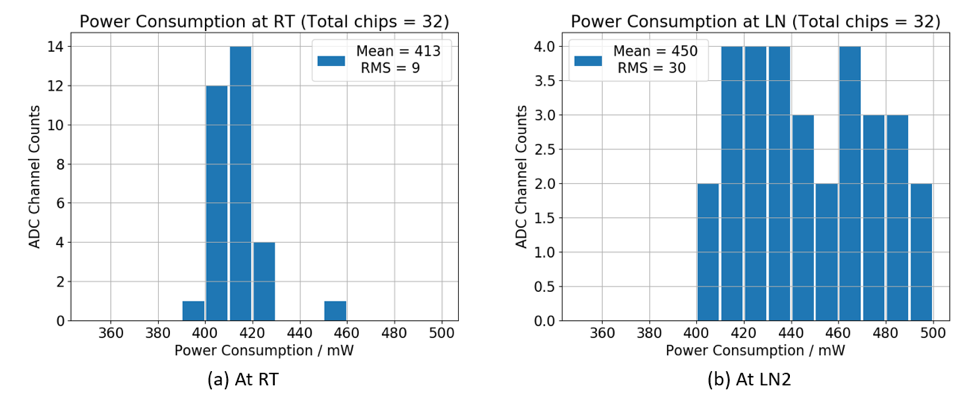
\includegraphics[width=0.85\linewidth]{figures/qc_power.png}
  \caption{Power consumption distribution.}
  \label{fig:qc_power}
\end{figure}

\subsubsection{Linearity Results with 2 Ms/s/channel Sampling Rate}
The results of the linearity and noise measurements at the nominal 2 Ms/s/channel sampling rate for the 33 chips are shown in 
FigureX (RT) and FigureY (LN$_2$). 
The QC tests are done with all 16 channels simultaneously connected to the signal source.
Due to the known SHA/MUX crosstalk issue, if the sample rate is 2MS/s per channel, the performance is expected to be worse. 
Another caveat is that the calibration of the ADC pipeline stages are not done for this result to shorten the testing cycle..
%The degradation is allowed because it is consistent to all chips, and additional test with 500 kS/s per 
%channel is also performed to confirm the degradation is caused by SHA/MUX crosstalk issue.  
%The ColdADC internally is 16-bit. The DUNE experiment requires 12-bit ADC is required by 
%DUNE experiment, ColdADC is truncated down to 12-bit by cut-off the lowest 4 bits. Meanwhile, in order to get ENOB, the coherency 
%frequency of sine wave is calculated for 12-bit ADC followed the equation of IEEE standard. 
Overall, the ColdADC performance is reasonably good, average of the worst DNL is 0.76LSB, average of the worst INL is 2.6LSB, 
average of ENOB is 10.0 bit and average of DC noise at 900mV is 0.68vLSB. In addition, the spread of these 4 key parameters 
among channels (or chips) is small.
Cryogenic test is performed as well with the same configuration,  Figure 7 shows the statistical result. 
By comparing Figure 6 and Figure 7, the linearity  performance of DNL, INL and ENOB do not show significant temperature dependence
 but the DC noise at LN$_2$ is smaller than at RT due to the suppression of thermal noise at cryogenic temperature.  


\section{Summary}  
%	\input{summary}

\clearpage
\newpage
\begin{thebibliography}{99}

%Citation from Introduction (Sec 1)
%

%
%Citation from Test Setup (Sec 2)
%

%
%Citation from Functional Testing (Sec 3)
%


%
%Citation from Performance Results (Sec 4)
%

%
%Citation from Issues Identified and Mitigations (Sec 5)
%


%
%Citation from Production Testing (Sec 6)
%


%
%Citation from Summary (Sec 7)
%


%
%Citation from Appendix
%



\bibitem{dunecdr} "LBNF/DUNE Conceptual Design Report",  \url{https://web.fnal.gov/project/LBNF/ReviewsAndAssessments/LBNF-DUNE\%20CD-1-Refresh\%20Directors\%20Review/SitePages/Conceptual\%20Design\%20Report.aspx}

\bibitem{montanari_35ton} First scientific application of the membrane cryostat technology, D.Montanari et al, \textit{AIP Proceedings 1573, 1664 (2014)} \url{http://scitation.aip.org/content/aip/proceeding/aipcp/10.1063/1.4860907}

\bibitem{genie} "The GENIE Neutrino Monte Carlo Generator", C. Andreopoulos, et al., Nucl. Instrum. Meth. A614, 87 (2010).



\end{thebibliography}



\newpage
\section*{Appendix}
\label{sec:appendix}




\end{document}
